\documentclass{cslthse-msc}
\setcounter{tocdepth}{4}
\setcounter{secnumdepth}{4}		
\usepackage[utf8]{inputenc}
\usepackage[english]{babel}
\usepackage{amsmath}
\usepackage{amsfonts}
\usepackage{amssymb}
\usepackage{amsthm}
\usepackage[table]{xcolor}
\usepackage{graphicx}
\usepackage[titletoc, header, page]{appendix}
\usepackage{todo}
\usepackage{float}
\usepackage[hyphens]{url}
\usepackage[hidelinks]{hyperref}
\usepackage{wrapfig}
\usepackage[within=none]{caption}
\usepackage{pdfpages}
\usepackage{svg}
\usepackage{listings}
\usepackage{color}
\usepackage{tikz}
\usepackage{scrextend}
\usepackage{tikz-qtree}
\usetikzlibrary{trees}
\usepackage{capt-of}
\usepackage{comment}
\usepackage{rotating}
\newcommand{\hilight}[1]{\colorbox{yellow}{#1}}

\definecolor{mygreen}{rgb}{0,0.6,0}
\definecolor{mygray}{rgb}{0.5,0.5,0.5}
\definecolor{mymauve}{rgb}{0.58,0,0.82}
\usepackage{colortbl}
  \definecolor{Lightgray}{RGB}{235,235,235}

\lstset{
breaklines=true,
language=SQL,
numbers=left,
numbersep=5pt,
numberstyle=\tiny\color{mygray},
frame=single,
basicstyle=\footnotesize,
captionpos=b
}
\newcommand{\bex}{BeX\textsuperscript{\textregistered}}
\renewcommand{\lstlistingname}{Algorithm}% Listing -> Algorithm
\renewcommand{\lstlistlistingname}{List of \lstlistingname s}% List of Listings -> List of Algorithms
\newcolumntype{H}{>{\setbox0=\hbox\bgroup}c<{\egroup}@{}}


\author{
	Alexander Söderberg \\
	{\normalsize \href{mailto:email@alexandersoderberg.com}{\texttt{email@alexandersoderberg.com}}}
	\and
	Max Åberg \\
    {\normalsize \href{mailto:aaberg.max@gmail.com}{\texttt{aaberg.max@gmail.com}}}
}

\title{Optimizing business intelligence
extraction speed from an
ERP-system’s database}
\subtitle{Master Thesis}
\company{Perfect IT BeX AB}
\supervisors{Lennart Söderberg, \href{mailto:lennart@perfectit.se}{\texttt{lennart@perfectit.se}}}{Alma Orucevic Alagic, \href{mailto:alma@cs.lth.se}{\texttt{alma@cs.lth.se}}}
\examiner{Per Andersson, \href{mailto:per.andersson@cs.lth.se}{\texttt{per.andersson@cs.lth.se}}}

\date{\today}

\acknowledgements{
We would like to thank Niklas Lindgren at \bex for giving us access to their systems and helping us with setting up a copy of their database system on our own machine for testing. We received great feedback, advice and hands-on experience during the whole process.\\

\noindent A big thank you to Alma Orucevic-Alagic, our academic supervisor without whom there wouldn't be a thesis, who gave us great support and pointed us in the right direction when we got stuck.\\

\noindent Finally, we would also like to thank Lennart Söderberg of \bex, who gave us this opportunity and together with whom we came up with this thesis. He also gave us invaluable feedback during the whole process.
}

\theabstract{
\noindent The popularity of cloud-based applications has increased the importance of performance optimized databases. In this thesis the database for a cloud-based ERP-system called \bex Online is investigated with the goal to optimize the generation speed of reports in the business intelligence functionality in the case system. The result is a set of recommended solutions to bottlenecks and inefficiencies found during the analysis, as well as suggestions for architectural improvements. Improvements to the generation speed of the business intelligence reports could be made in query tuning, index fragmentation, maintenance planning and table partitioning. Although database optimization is a widely researched subject it remains a complex and time consuming process, and the thesis concludes with a recommendation of areas that need to be further investigated.
}

\keywords{MsSQL, ERP, BI-report, query tuning, index }

%% Only used to display font sizes
\makeatletter
\newcommand\thefontsize[1]{{#1 \f@size pt\par}}
\makeatother
%%%%%%%%%%


\begin{document}
\makefrontmatter

\chapter[Introduction]{Introduction}
Computerized database systems have been in existence for over 50 years now and have quickly replaced the manual filing system, especially in larger companies. One of the first database management systems (DBMS) was the SABRE system by IBM that was built to help American Airlines manage its reservation data, Head \cite{Head02}. In the seventies the relational database model (RDBM) was presented but it wasn't until 1986 that the Structured Query Language, SQL, became a standard, ISO/IEC \cite{sql1}. \\\\
Database performance tuning has become increasingly important in recent years. In 1984 the main optimization techniques focused on rewriting queries in order to fetch data in a more efficient way , Jarke \& Koch \cite{jarke1984query}. This is still a very relevant technique, but today database optimization involves more areas such as indexing, table partitioning, execution planning, in-memory solutions and even switching to a completely different kind of database system.\\\\
Most software companies are striving to make their services cloud based in order to meet the increasing demands from the market of availability, accessibility and reliability. Users have got used to having mail, music, documents, pictures, etc in the cloud. The heavy load and increasing size of databases has put additional pressure on applications to have good performance.\\\\
Hence, there exists an increased market demand for cloud based software and the market pull today is on tools for businesses that exist in the cloud. Most tools have been available for a couple of years already, notably Microsoft Sharepoint that has been available since 2001. There is however one market that has been lagging behind, the ERP-market, Wilson \cite{wilson}. According to a study made in 2013, Gartner \cite{Rayner13}, only 2\% of survey respondents used a cloud based ERP-system. However, over half of the respondents said that they have planned to make the move within the next five years. One of the big attractions of Cloud ERP is, besides convenience, cost. Regular ERP implementations can last for years and require massive investments. According to Christine Hansen \cite{Robb14}, cloud ERP reduces the time and cost of maintaining infrastructure. By spending less money on IT, lower costs of product delivery can be achieved and enables businesses to get a competitive pricing edge and/or higher margins.\\\\
In 2014 Oracle introduced Oracle Customer 2 Cloud program, stating that they had 29 million cloud users, Kanaracus \cite{Kanaracus2013}. Microsoft has also been slow at adopting the cloud for its ERP solutions, but are now pushing their partner community for hosting its cloud-based SaaS solution Microsoft Dynamics. The biggest player on the market seems to be SAP, who claims to have over 35 million users. The large investments made by these companies shows that there is indeed a strong belief that ERP needs to be in the cloud.\\\\
As more and more services are made available in the cloud, more and more data is available and users are starting to become used to being presented data in meaningful ways. This is especially true for businesses. Steve Farr \cite{RobbOkt14}, product marketing manager at Tibco Software, noticed that in web-based forums about ERP, business intelligence is one of the most popular trending subjects. According to Farr, ERP systems are unattractive since they are expensive to implement and in general the market is a replacement market where everyone already has one. Most systems have broadly similar functionality which makes it hard for VARs (Value Added Reseller) to get clients to throw out an old system for a new one. To get ahead of the competition, Farr explains that VARs selling ERP are trying to use Business intelligence (BI) as a way of beating the competition. BI environments however, require enormous processing resources to support the large volumes of data that needs to be analyzed in order to identify trends. This means that the BI environment needs to analyze data from almost all parts of a target system, which places pressure on the business resources , Thompson \& van der Walt \cite{Thompson10}.\\\\
One of the biggest challenges that companies developing cloud solutions has to tackle is scale. One of the key points of the cloud is that users don't have to worry about how their system is hosted physically, since this is done by the supplier of the service. But the supplier is not very likely going to give separate resources to each client, since this isn't very cost effective. In fact, some industry experts claim that a service isn't a true cloud service unless the technical implementation of the service is that all users share the same physical resources, i.e. all customers access the same resources from the same cloud, Netsuite \cite{Netsuite15}. This has started a performance race in the cloud industry. By making sure that the service is using the best technologies and is programmed in the best way, suppliers can lower cost by needing less hardware, as well as delivering a faster product to their customers. This need has given rise to many new technologies in recent years, especially in the database industry.\\\\
Ten years ago a classical relational DBMS was the preferred solution when building an application. This type of database has been used for more than 30 years and has been one of the core products from giants such as Microsoft and Oracle. But when the content of databases started to become more and more complex with more and more relations, new types of databases emerged to combat complexity and performance issues, Rouse \cite{Rouse2011}. This trend has been called NoSQL, which stands for "Not Only SQL" or "No Sql"-at all, Fowler \cite{Fowler12}. Whichever definition one may chose the main point behind NoSQL is that a table is not the best data structure for all sorts of data. Rather, applications can experience a major performance increase by using more appropriate data structures for their type of data, e.g. hash maps, node trees or graphs. Some developers even propagate getting rid of schemas for data objects, aiming to let the data structures be as versatile as possible, Fowler \cite{Fowler12}. In response to the NoSQL trend, Oracle and Microsoft have in turn released powerful technologies that put parts of the database in RAM, making it much faster than before.\\\\
Today's users expect their applications to be fast and there are certainly a lot of technologies for developing fast web applications. For companies that develop cloud services, there is no longer an excuse for poor performance.\\\\
In this master thesis, an analysis of a ERP system is performed in order to optimize generation of different client sales (business intelligence) reports. Hence, in the background, chapter \ref{sec:background}, the case company's software solution is discussed. In research questions and methodology, chapter \ref{chap:3}, the thesis research questions are presented.

\chapter{Background}\label{sec:background}

\section{Background}

\subsection{Database Optimization}
Database optimization aim to increase the performance of database systems. One way to improve performance is by altering how the database is designed and configured. As well as how queries are composed, or by changing the environment that the database system runs on, i.e. operating system or buying better hardware. In 1984, Matthias Jarke and Jürgen Koch \cite{jarke1984query} wrote an article about how to improve the performance of relational database systems. In 1984, the focus was on query optimization as there was no comprehensive survey on database optimization. The problem was resolved by reviewing the query optimization techniques in a common framework of relational calculus, Jarke \& Koch \cite{jarke1984query}.\\\\
For a long time database optimization was equivalent to query optimization, but today database optimization involves other fields as well. The most common areas to work with when optimizing a database are indexing, query planning and statistics, data redundancy, changing database types, adding in-memory solutions and distributed database systems, Nevarez \cite{Nevarez}.\\\\
Poor indexing is one of the most common problems when a database has performance issues. The indexes enable database systems to find the right row in a table faster and to have this properly set up is naturally very important. It is also important to maintain these indexes since the tables in a database often change over time and the indexes might become outdated.\\\\
Writing SQL queries is like writing questions. If these questions are poorly stated the answer will take longer to generate. This is designed so that a user doesn't have to worry about how the data is actually retrieved from the tables. Optimizing queries is most often about making sure that the questions are asked in the best way, e.g. how to join different data together. Equally important is the way the queries are executed and that the database system has appropriate information to do this in the best way. Since there can be thousands or even millions of different ways for a database system to execute a query it is important that the system has good statistics about the database tables and relations. By makings sure these statistics are up to date and correct the database system can quicker and more accurately choose a query execution plan with high performance, Nevarez \cite{Nevarez}.\\\\
In the last five years NoSQL solutions have started to become a serious competitor to traditional relational databases. They were created with the mindset that modern software, web applications in particular, are not best represented by a relational SQL database with tables and rows. The idea in most of these No-Sql systems is that data is best saved as objects or in other data structures. One of the biggest types of NoSQL databases is a graph database, which is designed so that relationships between data is as important and as easily queried as the data itself. These database systems has been proven especially powerful when performing searches that needs to find relationships, e.g. the friends of friends of friends-problem in social media. In a study by Vicknair et al. \cite{vicknair2010comparison}, these kind of problems were shown to be solved more than 13 times faster in graph databases than in an SQL database. However, when searching for a specific value in the database the SQL database was approximately 110 times faster.\\\\
When relational database systems were originally designed, memory, better known as RAM, was very expensive and small compared to disk space. Therefore the systems were designed to use as little memory as possible by fetching only the necessary from disk into memory. Today memory has increased while its cost has decreased. Many of the current DB systems take advantage of this, especially NoSQL systems. The biggest database system providers in the world, Microsoft, Oracle and IBM, have each released own versions of in-memory databases. It has been shown in a test done by McObject \cite{mcobject} that read and write speeds were 420 times faster when the database was in RAM rather than on disk.\\\\
When a system starts to receive a lot of traffic a single server might not be enough to keep up to quality requirements regarding performance and multiple servers have to be used. This calls for the need of a distributed database system. By keeping a single database on multiple physical locations the traffic load can be handled and directed to the least busy server.

\subsection{Case Company}
Perfect It BeX AB was founded in 2007. In the beginning the company made business extensions such as B2B, e-commerce and retail for the Microsoft Navision ERP \cite{Navision}. Eventually the case company started developing a new ERP-system in order to accommodate their extensions since the technologies on which Navision was based did not fulfill desired requirements. In 2010 the company released three products; \bex Online, \bex Retail, and \bex B2B. \bex Online is the main product on which the other products rely. It is a completely cloud-based ERP-system specialized for the retail industry. The main functionality in \bex Online are:

\begin{itemize}
\item Financial tools
\item Sales administration \& handling
\item Purchase handling
\item Inventory and Warehousing
\item History and Business Reports
\end{itemize}

\noindent In recent years, Perfect It has experienced an increasing demand from customers for better business intelligence capabilities. In response to this the company has improved the business intelligence report functionality in \bex Online, to be able to give a wider range of different financial key values. According to the company's CEO, being able to offer customers appropriate BI tools, is key to staying competitive. However, generating some of the reports can take a relatively long time, especially for bigger clients whose systems have large amounts of data and are further growing.

\subsection{BI-reports}\label{sec:BI}
Business intelligence is analyzing large amounts of raw financial and company data and transforming it into meaningful and useful information on which a company can base their decisions, Gartner  \cite{bintelligence}. This often involves different software solutions specialized for these tasks. One of the most common types of business intelligence is reports that shows accumulated or compiled data. In the case company's system there are features for business reports in the following areas:

\begin{itemize}
\item Sales
\item Purchasing
\item Warehousing
\item Accounting
\end{itemize}

\noindent In each area there are several different kinds of reports depending on what key values a user are looking for, e.g. Sales has 26 different kinds of reports. These kinds of reports are referred to be at the top layers of the BI architectural stack together with analytics and dashboards, Evelson \cite{Evelson10}. They perform the first step of mining and arranging unsorted data sets into arranged and understandable data, and it is on these kinds of reports that further BI analysis can be based.\\\\
Perfect IT delivers services to mostly retail and e-commerce clients. There are 48 BI-reports available and used by the clients. The BI-reports that are of the most importance are the ones that generate statistics for sales and purchasing (Sales and Purchase in Figure \ref{fig:BI} in Appendix \ref{sec:appTabIll}), where the latter-mentioned is used for purchase decisions. These areas consist of several BI-reports where some of these cause inconvenience in the form of performance stalling. 

\section{Problem description}
Perfect IT BeX AB was motivated to collaborate with academia in order to investigate the current performance issues with respect to the generation speed of the business intelligence-reports. The key issue is improving and maintaining a high performance level in a database that is constantly increasing in size. Since the business intelligence-reports collect data from all parts of the system, investigating their performance implies looking at the whole system.

\section{Thesis Goals} \label{sec:goals}
The goal of this thesis is to identify issues related to the problem, and to propose a solution for speeding up the generation of BI-reports in Perfect IT BeX AB's product \bex Online. In order to speed up the BI-report generation the system processes responsible need to be identified and further examined. The proposed solution needs to take the constraints of the current system and its future growth into consideration. Hence, the proposed solution needs to be scalable. Taking into account that Perfect IT BeX has one physical server, the scalability should be vertical, Hill \cite{scalability}, since the company will provide the system to more clients in the future. Vertical scalability is to add resources to a single node and in this case it could be the addition of CPU or memory to the server.\\\\
In order to make the above optimization possible, the following goals have been established:
\begin{enumerate}
\item Identify the most common causes to database inefficiency.
\item The current processes behind generation of the BI-reports must be identified and mapped in order to identify bottle-necks and inefficiencies.
\item Propose \& test possible solutions and use the "Problem Solving Research"-process, Höst et al. \cite{regnell}, as the academic approach.
\item Analyze \& compare possible solutions to determine which fulfills the needs of the case company.
\item Propose solutions to the performance problems in \bex Online and perform a final analysis to determine if the case company's goal was met.
\end{enumerate}
  
\section{Scope} \label{sec:scope}
Because of the problems and goals described in the background the focus should be on the following main areas of investigation:
\begin{itemize}
\item Query tuning
\item Execution plan tuning
\item Index tuning
\item Database execution statistics
\item In-Memory OLTP
\item Plan caching
\end{itemize}
Due to the limited time frame of this thesis, all of these areas won't be explored. With respect to this and the company's preferences the following focus areas were decided upon: query tuning, index tuning, "In-Memory OLTP"-solutions and database execution statistics.

\section{Limitations}\label{sec:limi}
The primary objective of the thesis work is to increase the speed of the ERP-system's business intelligence reporting module by optimizing the database. The underlying database implementation is used by all parts of \bex Online. This means that the following limitations to the developed solution must be in place.

\begin{itemize}
\item The solution must not adversely affect any functionality in \bex Online.
\item The solution must not redesign the database, as this would affect the other parts of the system.
\item The solution must work with the current implementation of \bex Online back-end.
\end{itemize}

\section{Related Work}\label{sec:related}
There has been many attempts to solve various issues related to implementing a large database system. Some of these attempts have completely redefined the classical definition of a database. The following subsections introduces areas and DBMS-techniques (Database Management System) with different angles to solve the problems mentioned in this thesis and several other issues.

\subsection{Database optimization in ERP}
In Kemper et al.'s article \cite{SAPR3}, common performance problems with DBMS and one of the largest ERP-systems, SAP, are investigated and solutions to these issues are presented. In the paper, main-memory management is discussed and the importance of configuring it correctly. The authors recommend allocating extended memory instead of using the shared main-memory. These strategies can be seen as early work in what in recent years have evolved into complete in-memory solutions. The importance of caching in order to reduce the load on the database server is investigated. However no recommendation is given on how caching should be performed, since the authors recommend that the database administrators decide this themselves.\\\\
In SAP there is a query optimizer that implements two techniques. Cursor caching and Caching data. Cursor caching reduces the overhead of calls to the RDBMS by, e.g. having all the queries that retrieve the matching tuples of the inner relation in a nested SELECT statement use the same cursor. The data caching is in SAP in order to avoid calls to the RDBMS altogether. The query optimizer doesn't rewrite queries, but instead reallocates resources to the areas of the system where the query has bottlenecks.\\\\
Different ways of monitoring and evaluating performance is shown in order to maintain the database. Processes to benchmark the performance is introduced. The main benchmarking process is called the SSQJ-tool. It can be compared to maintenance planning but it functioned more as a tool to find issues before release of a system, instead of a tool for constant benchmarking and maintenance.

\subsection{DDB}
1988 Stonebraker \cite{DDBMSvsCDBMS} predicted that distributed database technology would impact the data processing the same way that centralized systems did in the 70's, making the centralized systems an "antique curiosity". Which of course is not entirely true, but with the progress of the modern technology more and more large companies need to expand their centralized system to take care of huge user- and performance-loads.\\  
Distributed databases differ from centralized databases in the way that the logical database is spread physically across a communications network to multiple locations/computer systems , McFadden \cite{DDBMS}. A distributed database system has several requirements to function as intended and provide the core functionality; share data. To start the network must allow users to share data, to be able to do so there must be a database management system at each remote node/site that coordinates the access to data, called DDBMS (Distributed Database Management System). The DDBMS provides a lot of functionalities that cover the requirements to share data, such as: \begin{enumerate}
\item Keeping track of where the data is located
\item Retrieve data from determined location without special actions by user
\item Query translation between different local DBMSs
\item Concurrency control, recovery and other management functions
\item Replication of data across the nodes/sites
\item Scalability as to growth in nodes/sites additions \begin{flushright}  Elmasri \& Navathe \cite{functionsDDBMS}, Buretta \cite{datareplication}   \end{flushright}
\end{enumerate}      
The functionalities provided by a DDBMS should cover four important transparencies; Location transparency, replication transparency, concurrency transparency and failure transparency. Meaning that the database provides a user with data from unknown physical location (user is unaware of data distribution), data that is replicated on several locations, simultaneous transaction execution without effecting performance and guarantee that all actions of each transaction is committed or else none is committed.\\\\
So why should databases be distributed? Well as earlier mentioned it improves performance as data and users grow in size. Businesses conditions such as; distribution and autonomy of business units, data communication costs and reliability, multiple application vendor environments, database recovery and the satisfying of both transaction and analytical processing, all encourage the use of distributed databases, McFadden \cite{DDBMS}.\\ Compared to centralized databases, most forms of distributed databases have numerous advantages, but also faces disadvantages:     

\begin{center}
\noindent\begin{minipage}[t]{0.5\linewidth}
    \begin{itemize}
    \item[] Advantages:
    \item{Increased reliability and availability}
    \item{Local control}
    \item{Modularity}
    \item{Faster response, for properly distributed data}
    \end{itemize}
    \end{minipage}%
    \begin{minipage}[t]{0.4\linewidth}
    \begin{itemize}
    \item[] Disadvantages: 
    \item{Complexity}
    \item{Additional software costs}
    \item{Zealous security}
    \end{itemize}
\end{minipage}
\end{center}
\begin{flushright}
Seydim \cite{advdisDDBMS}
\end{flushright}
To be able to reach the advantages with DDB the system needs to be properly implemented. Depending on the usage, the data distribution among the different nodes could be designed in several ways. Additionally the DBMS may need to process data responses from several different sites, making it crucial for the DBMS to interpret queries optimally, leading to a big responsibility at the intelligence of the DBMS and the user formulating a query. 

\subsection{OODB}
During the same time as the DDB had its goals to overpower the centralized systems, the need to perform complex data manipulations grew. A new generation of database applications generated a demand to meet the requirements beyond the characterized relation database systems, Bagui \cite{OODBMS}. Using the already conventional relation database systems for these advanced applications, such as computer aided designs (CAD), quickly exposed the drawbacks of RDBs, Bertino \cite{OODBMSshortcomings}. Thus object-oriented database (OODB) systems derived to satisfy the demands to represent real world entities.\\\\
The OODB paradigm follows the paradigm for object-oriented programming languages such as Java. It's based on a number of concepts; Object, Identity, Class, Overriding etc., Atkinson \cite{OODBMSparadigms}. The entities in an object-oriented data model are represented by objects. These object have a state and a behavior, which are defined by the values of its properties/attributes and the methods that operate on the state of the object respectively. Properties can have a primitive value, such as strings and integers, and non-primitive objects that in turn is composed of a set of properties. Which enables objects to be recursively defined in respect of other objects. The objects are uniquely identified by a system-defined identifier called OID. Objects with the same behavior and state are organized into classes and can be an instance of one or several classes, Banerjee \cite{OODBMSclasses}. Classes are in turn organized in class hierarchies where subclasses inherit methods and properties from the superclass. Subclasses can have specific properties and implemented methods as well as have the possibility to override the inherited properties and methods from the superclass.\\\\
The object-oriented technology was expected, as DDB, to revolutionize the database technology. But OODBs lack certain basic features that users have become accustomed to. 
The advantages and disadvantages of OODB are numerous, therefore only a few will be featured in this section. The advantages and disadvantages are compared to the conventional relationship database.
\begin{center}
\noindent\begin{minipage}[t]{0.5\linewidth}
    \begin{enumerate}
    \item[] Advantages:
    \item{Allow user defined abstractions}
    \item{Eliminate the need of user defined keys}
    \item{Reduced need for \texttt{JOIN}}
    \item{Performance gain compared to RDB}
    \end{enumerate}
    \end{minipage}%
    \begin{minipage}[t]{0.6\linewidth}
    \begin{enumerate}
    \item[] Disadvantages: 
    \item{Interoperability between RDB and OODB }
    \item{Minimal query optimization and performance tuning}
    \item{Authorization concerns}
    \end{enumerate}
\end{minipage}
\end{center}
\begin{flushright}
Bagui \cite{OODBMS}
\end{flushright}
\paragraph*{Advantages}\mbox{}\\\\
\textbf{1.} The user of an OODB is allowed to create and define new data abstractions. Meaning the user can create new classes with methods and attributes, inherit from superclasses, create instances with unique identifiers, load and run methods etc., Kim \cite{userdefinedabstractions}.\\ \textbf{2.} With the help of the OID object uniqueness is guaranteed. Resulting in eliminating the needs of user defined keys. Therefore it's not possible to modify the OID by applications and two object are different even if they have the same value for all their properties and structure, Khoshafian \cite{identity}.\\\textbf{3.} The OODB enables navigation through object structures and path expressions in object attributes. These path expressions can reduce the need for joins of classes, Kim \cite{userdefinedabstractions}.\\\textbf{4.}
\begin{addmargin}[1em]{0em}
\textbf{a)} If the domain of a value of an attribute in an object is another object, the value references the latter object (OID). Thus if the first object is retrieved the latter object can be instantly retrieved by the first objects attribute value.\\
\end{addmargin}
\begin{addmargin}[1em]{0em}
\textbf{b)} When OODB objects are loaded into memory the objects OID is converted into memory pointers. Making repeated navigation through linked objects loaded in memory dramatically faster, Kim \cite{userdefinedabstractions}.\\
\end{addmargin}
\paragraph*{Disadvantages}\mbox{}\\\\
\textbf{1.} OODBs are not compatible with RDBs, there's a need for a migration path. The architecture and data models between OODBs and RDBs are not yet unified, making it difficult for these systems to coexist, Kim \cite{userdefinedabstractions}. \\\textbf{2.} Since OODBs often contain a lot of user defined classes and new types the optimizer can have a hard time to predict the "relation" between classes and might assume that a class is a subclass to a faulty superclass. In addition complex methods, objects and encapsulations add complexity through complex path expressions in the query processing. Due to these problems object-oriented query optimization is still in research stage, Erlingsson \cite{OODBqopt}. \\\textbf{3.} Unlike RDBs, most OODBs don't support authorization, making privileges on data nonexistent, Kim \cite{userdefinedabstractions}.\\\\
Unfortunately the phrase OODB has become a faulty term. The weaknesses has brought the OODB technology to being more of a constant storage of object-oriented programming language than database system. The OODB technology has not met its expectations to provide important features to the complex applications it was meant to help currently the disadvantages outweigh the advantages, Bagui \cite{OODBMS}.

\subsection{Neo4J \& Graph Databases}
Neo4J 1.0 was released in February 2010, NEO4J blog \cite{Neo4J10}. It is a graph database that stores its data as nodes and relationships. Neo4J was developed to counter a new scaling problem. Applications that handle entities, such as people, do not grow linearly but exponentially, since the more entities there are, the more relationships there are. Graph databases were developed with the philosophy that relationships are just as important as the data stored. So what would traditionally be stored as a table or even as a row in a table is in Neo4J stored as a data structure (node) with properties and relationships to other nodes. This is especially powerful in path operation problems like the "friend of a friend of a friend..."-search problem in social media platforms. Finding friends of friends of friends in a relational database involves emulating path operations by recursively joining data sets. This can cause query latency and memory usage to grow unpredictably, especially in large data-sets. In a graph database, relationships are stored physically on disk. This means that in a query, one can look at the relationships, which are first-class entities, right away, instead of having to find them at runtime. Different kinds of nodes and edges can also be used to add many layers of meaning. \\\\
One of the biggest argument against these types of databases is that it is bad at handling large sequential data sets. If a range of data needs to be iterated every single node needs to be visited and searched for the next node which is slower than just visiting every entry in a sequential table. This also means that searches for specific values can be slow. In 2010, Vicknair et al. \cite{vicknair2010comparison} studied the performance differences between a graph database, in this case Neo4J, and the relational database MySQL. They set up twelve databases of each system with different database sizes and then measured the time in milliseconds of different queries. When performing traversal queries, the graph database was faster by a factor of 10. During a query for full text character search, i.e. finding a specific value, MySQL performed better at a small scale, but scaling upward Neo4J outperformed MySQL with sometimes up to 168 times the speed.

\section{Contributions}
This section presents an overall picture on which areas Max respectively Alexander were responsible for as well as which parts of the written thesis they relate to.\\
Both were equally responsible for the structure of the report as well as the use of \LaTeX and git as VCS, seeing that the two had equal experience in the editor and the revision control system. The literature research was also done equally and was mostly made in the beginning but modified together with updates during the reports lifetime.\\\\
Alexander had former knowledge and encounters with the company, thus initial contact and correspondence with the company stakeholders ended naturally up in his responsibility. Alexander had therefore a much better overview of the company's background and naturally the related chapter in this report became his responsibility. The written part of the background chapter was consequently mostly written by Alexander, except with some collaboration from Max to establish the thesis goals and scope. The methodology and work development description in chapter \ref{chap:3} was Max responsibility and was developed during the reports whole lifespan.\\
In the approach chapter Max wrote the company's technical system description while Alexander's responsibility was focused on research of indexing and in-memory solutions for databases. The theory section of the approach chapter was collaborated together were Max wrote about query optimization and Alexander of above mentioned areas.\\
In the analysis section both thesis students wrote on the parts they had worked on in the previous section. Hence Max was responsible for analyzing and dissecting the stored procedures in the system as well as experimenting with the different parts of the company's database. Alexander's engagement was concentrated on investigating the databases indexes along with memory possibilities and future maintenance of the possible solutions.\\           
The solution recommendations in chapter \ref{sec:proposedsoluton} were established by compiling the formerly individual parts and writing the chapter as a team. The same goes for both the discussion and the conclusion. 
      
\chapter{Research Questions \& Methodology}\label{chap:3}

\section{Research Questions}
The research questions of this thesis were formulated in relation to the thesis goals in section \ref{sec:goals} and the scope in section \ref{sec:scope}. The thesis is formed to explain and answer the following research questions:
\begin{enumerate}
\item	How does the current system function and what are the bottlenecks, in particularly regarding the BI-report generation?
\item 	What are the most common approaches for improving database performance, with regard to index fragmentation, query tuning and In-memory-solutions?
\item	What optimization solutions are best-fit for the case company with regards to the goals, scope and limitations?	
\item	How can the proposed solution be implemented in Perfect IT \bex AB's current system?
\end{enumerate}

\section{Methodology}
This thesis is of a problem solving nature and should continuously adapt to changing conditions. The methodology used should therefore preferably be flexible in the sense that iterations and unforeseen obstacles do not prevent the thesis' outcome. A methodology that provides valuable support and is intended to improve something while studying it is action research, Robson \cite{robson}. Action research begins with an observation phase that identifies and clarifies the problems that are present, for this thesis that is presented in chapter \ref{sec:background}. In chapter \ref{sec:proposedsoluton} the next step in action research is stated, a proposed solution to the problem(s).\\

\noindent After implementing the proposed solution the next phase is the evaluation. The evaluation is made to verify the implementation in its context, to analyze and reflect on how it works in its integration. The whole action research is an iterative process and is based on the evaluation. Accordingly to Höst et al.    \cite{regnell} an evaluation is hard to keep unbiased, since the ones doing the critical evaluation are also the ones that performed the research. To counter an unbiased evaluation, some evaluation criteria were established based on the above mentioned goals in section \ref{sec:goals}. To ensure that all of the stakeholders goals are met this thesis will on a regular basis be reviewed both by supervisors at Perfect IT and at LTH.

\section{Work}
First of all an acquaintance of Perfect IT BeX AB's system needed to be established. In conjunction with the examination of the current system and its parts a literature research was performed. The area this research treats is extensive and the research done is almost indefinite. Therefore the literature research scope needed to be narrowed with its base in the currents systems examination.\\\\    
To find the literature and related work Engineering Village   \cite{Enginvillage} and Google Scholar \cite{Googlescholar} together with DBLP   \cite{DBLP} was used. A lot of time was dedicated to find relevant literature and information for this thesis and at the same time examine if the ideas established during the system examination phase were possible and solid solutions.\\\\
Using the paper written by Gruian and Lekebjer on formatting a master’s thesis   \cite{Reportmall} and guidelines from the book by Höst et al.    \cite{regnell} the initial work on the master thesis report was conducted.\\\\ 
To support the thesis's scope, seen in section \ref{sec:scope}, and to explain to the reader how and why the proposed solution is of interest, an approach was established in chapter \ref{sec:approach}. The approach begun with examining the current system and its components to unravel the complications and the areas that needed further investigation. Once that was done the thesis needed theoretical background to support and target the found problems.\\
The next step was to analyze the system and see if the initial ideas and theoretical solutions had a possibility of reaching an improvement.
From the analysis several solutions were found to be applicable and a proposed solution, as discussed in chapter \ref{sec:proposedsoluton}, was created were solutions are further explained, how they may be implemented and further recommendations are stated.\\
Last but not least a discussion about the thesis's results and discoveries was created. The discussion in chapter \ref{sec:discussion} also treats extrapolations, expected impact and negative/positive experiences during related work carried out.
The whole thesis is then concluded, see chapter \ref{sec:conclusions}, to summarize the findings, possible improvements and future recommendations.\\\\
The work done in the theoretical part, the analysis and in the proposed solution were done in iterations. Alongside these iterations further literature research and results added progress to this master thesis.\\
An overview of the different areas of the work carried out throughout this master thesis can be viewed in Figure \ref{workflowgrapgh}.

\tikzstyle{every node}=[rectangle, draw, fill=blue!20, 
    text width=10em, text centered, rounded corners, minimum height=4em]
%[draw=black,thick,anchor=west, fill=blue!10,style={draw,-latex}]
\begin{figure}[H]
\begin{center}
\begin{tikzpicture}[%
  grow via three points={one child at (2.7,-2.0) and
  two children at (0.5,-0.7) and (0.5,-1.4)},
  edge from parent path={(\tikzparentnode.east) -| (\tikzchildnode.north)},
  edge from parent/.style={draw,-latex}
  ]
  \node {Analyze the problem}
    child { node {Perform research to understand the core issues}
		child {node {Use research to analyze the case system}
			child {node {Experiment with solutions to the issues}
				child{node {Propose recommended solutions}}}}    
    };
\end{tikzpicture}
\end{center}
\caption {Work flow graph}
\label{workflowgrapgh}
\end{figure}         

\chapter{Approach}\label{sec:approach}

\section{Technical System Description}
Perfect IT delivers web-based business systems and services specialized for the retail industry. The \bex Online ERP-system is distributed as a SaaS-solution and all clients share servers which makes it a true cloud based service. The clients access \bex Online's front-end through a web browser. \bex Retail and \bex B2B are connected directly to \bex Online's back-end.
The database for \bex Online is a Microsoft Server 2014 Web Edition.
\begin{figure}[H]
\vspace{-15pt}
  \begin{center}
    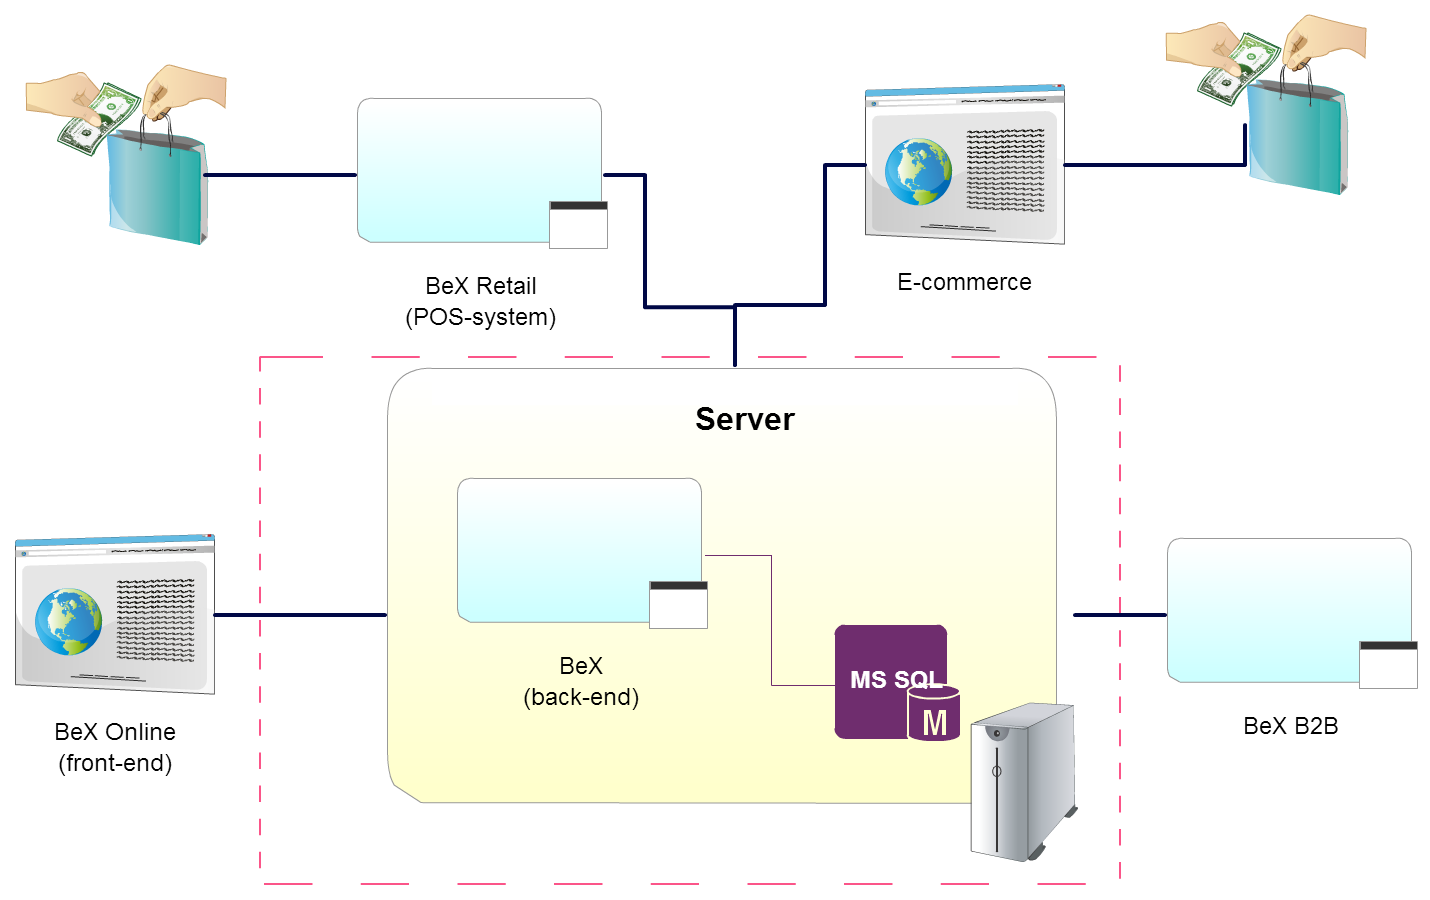
\includegraphics[scale=0.3]{Pictures/Systemdesc.png}
  \end{center}
  \caption{Context diagram of Perfect IT's system}
  \label{context}
  \vspace{-15pt}
\end{figure}
\noindent The dashed section in Figure~\ref{context} are the components that are of the most interest for this thesis and will be more thoroughly described than the other system components.

\subsection{Components}


\subsubsection{Server}
Currently all the client instances of \bex Online are placed on a single server hosted by a third party hosting company. This server also hosts the database system.
The technical specification of the server is specified in Appendix \ref{sec:Genviron}

\subsubsection{\bex Online}
\bex Online is a cloud based ERP system and has a front-end built with HTML5, CSS and JavaScript and a back-end written in C\# and .net with Web forms.
Every client has their own instance of the system and every client can have multiple users. \bex Online acts as a central hub for e-commerce and point of sale (POS) systems. It receives traffic 24/7 from clients interacting with the system as well as from e-commerce and POS platforms. Thus there are requirements on reliability and performance.

\subsubsection{Database}
The database system used is Microsoft SQL Server 2014 Web edition. It has a maximum data capacity of 524 PB, maximum ram usage of 64GB, maximum CPU capacity < 4 socket or 16 cores. All clients are on the same SQL Server 2014-license but have their own unique instance of the database-system with only their data.  Perfect IT has around 40 clients, all with different database sizes ranging from approximately 5GB of data to approximately 90GB of data in their database. The database is an RDBMS and is run on a Microsoft SQL Server 2014-license using OLTP and the size of all the clients' databases together is approximately 350GB.

\paragraph*{Tables}\mbox{}\\\\
For this thesis Perfect It BeX AB has made available a copy of one of their biggest client's database. To ensure the clients privacy, and the privacy of the clients customers, all sensitive data has been removed. \\ 
The default schema is called \textit{dbo} and consists of a total of 254 tables, including some views for big data queries. Many tables are large, considering the amount of rows, where the largest consists of approximately 10.5$\times 10^6$ rows and 80 columns. This table stores the data associated with every business transaction made by the system from the start of using this system. The tables form a complex relation to each other and the references are many (as seen in Appendix \ref{sec:appTabIll}, Figure \ref{fig:ER}). In the visualized database reference schema there are tables not referencing any tables at all.\\\\
There are also tables needed by third party applications and API's that also are stored in the database and can be seen in the bottom part of the visualized database reference schema mentioned above. Some of the BI-reports have their own tables in the database, due to an early attempt to optimize the BI-report generation by storing the result of the latest query. Meaning that if the same query queries the result is already stored and doesn't need to be looked for. This is saved by user so there can be multiple search results from different users in these tables.

\paragraph*{Stored procedures}\mbox{}\\\\ 
Stored procedures are subroutines that are available to applications that access relational database systems. Stored procedures are used as centralized logic and can therefore be used by all applications that share the system. These subroutines can include both SQL statements and host language statements, meaning that it can exist external procedures that has nothing to do with SQL. Often extensive and complex SQL queries, that require a lot of processing and are often being used, are moved to stored procedures for reuse, Harrison \& Feuerstein \cite{StoredProcedures}. It's important to know that stored procedures both bring advantages, e.g. stored procedures are cached, and drawbacks, e.g. stored procedure code is not as robust as app code. Subroutines such as stored procedures should therefore only be used when and if the implementer possess a deep knowledge of the system that is to be affected. It's for example bad practice to store all procedures as stored procedures for the benefit of the cache-utilization.\\\\
The database in this thesis had a total of 59 stored procedures treating repetitive procedures by the database mainly for the sales part of the system and the BI-reports (there's also a subroutine for locking crucial information, with respect to concurrent execution). These subroutines do not contain any host language statements and/or external procedures, but only consists of complex SQL statements. They are present in the system, as mentioned above, to make the execution and processing less demanding, as they are often used in \bex Online.

 
\section{Theory}\label{sec:theory}
In order to understand why a database might not perform optimally, the following theory was used.

\subsection{Index Fragmentation}
Index fragmentation is one of the most common problems in a relational database. Two kinds of fragmentation can occur, internal index fragmentation and external index fragmentation. The easiest way to explain index fragmentation is by imagining the SQL database as a phone book. At the very end of the book you have a few pages containing a table with indexes of all the entries sorted by last name. This is fine in a static environment such as a phone book but causes problems in a dynamic environment.
Since people can be added to the phone book there must be space available after each column in the index, as well as in the pages in the phone book. This is called the \emph{fill factor}. A page can still run out of space and when this happens SQL Server has to add a new page, but it can't add it at the correct place because the book is already bound. So, it adds blank pages at the very end. This causes two problems, pages with a lot of unused space and pages that are out of order. The first problem is what is referred to as \emph{Internal Fragmentation} and the second is \emph{External Fragmentation}. Internal fragmentation will of course also occur when deleting entries since that leaves "blank space" on the page, Ozar \cite{Ozar12}.

\subsubsection{How fragmentation affect performance}\label{sec:indexbad}
At first, internal fragmentation might seem like a good thing. If the phone book has a lot of blank space on every page to start with, adding entries would be super easy and there would be no need for adding more pages later, causing external fragmentation. This is true, but when the number of extra pages needed in the phone book to allow for a lot of blank space is considered, the inefficiency of it becomes apparent. Going through a 100\% filled 1000 paged phone book is much faster than a 90\% full 1100 paged phone book. So in this example, every time SQL Server needs to scan the index, it would take 10\% longer. Another problem is that the lowest unit for caching in SQL Server is not a record, but a single page (8kb), which means that all the empty space must be cached as well. \\

\noindent External fragmentation often makes reading the database non-sequential, i.e. it cannot be read in order but must be read in random order. This is especially bad in classic magnetic hard drives where the reader head must move around to multiple locations on the drive. Some magnetic hard drives only get 1\% of their sequential reading speed when performing random reads, OBrien \cite{Toshiba12}

\subsubsection{Measuring fragmentation} \label{measurefrag}
In Shubho's article \cite{Shubho09} he explains how to measure index fragmentation if index fragmentation has occurred. By executing the script in Algorithm \ref{See DB-Fragmentation} in Appendix \ref{appCode}, index fragmentation is analyzed on every table in the database and presented in a table with an internal and external fragmentation value. \\

\noindent According to Shubho \cite{Shubho09}, only tables with an internal fragmentation value of less than 75 and/or an external fragmentation value of more than 10 should be considered as fragmented, which this code takes into account.

\subsubsection{Reorganize vs. Rebuild}\mbox{}\\
Both rebuilding and reorganizing are built-in operations in SQL-Server 2014. These are two different operations that both reduce the fragmentation of the indexes. Reorganizing is the more lightweight of the two operations. It fixes the indexes as well as physical reordering of pages and applies any previously set fill factors. Rebuilding builds up a completely new structure for the index. It also allows for a new fill factor.\\
The advantage with reorganizing over rebuilding is that it can be aborted midway, while a rebuild must roll-back after an abort. Usually, in most SQL-systems, a rebuild can't be done while the SQL-server is online. This can be done in MS SQL Server Enterprise edition, Little \cite{Little13}.

\subsubsection{Is it always a good idea to fix fragmentation?}
According to Brent Ozar   \cite{Ozar12} fixing fragmentation can cause more damage than keeping fragmented indexes. Often administrators try to fix fragmentation by using a low fill factor, say 50\%. This would mean that half of every page would be blank, which would make writing really fast. Reading however, would be twice as slow. Another common mistake is to rebuild every single index in the database, even though some tables might not had a single write since the last time. This is a problem because defragmenting indexes causes SQL Server to write to the transaction log. The bigger a log is, the longer log backups and restores take.\\\\
Another important factor is that external fragmentation mostly causes problems when the database is stored in disc, since classical hard drives are slow at random reading. If the database is instead stored in memory, which is almost as fast at random reading as sequential reading, external fragmentation won't be as big an issue.

\subsection{Query optimization}\label{sec:qopt}
Query optimization is often associated with altering and optimizing the logic and code in the SQL statements. Even if this is true, by tuning the actual SQL statements an optimization can be accomplished, it's done with respect to the execution plan. Query optimization can also been seen as mapping of the logical query operations to physical operations that the execution engine can execute. It does this by implementing a number of algorithms, which the query optimizer must choose from when formulating an execution plan. In summary a query optimization is actually a strategic manner to optimize the execution functionality of the execution engine, Nevarez \cite{Nevarez}. \\\\ 
The purpose of the query optimization is to provide a good enough and hopefully optimal execution plan. In order to do so a query must go through a query-processing process as can be viewed in Figure~\ref{fig:qpp}, which is a recreated illustration from Nevarez's book \cite{Nevarez}. But before optimizing a query, the SQL Server first checks if there is an execution plan in the cache for the SQL batch. Since the query optimization is a relative expensive operation, an available execution plan in the cache entails that the optimization process can be skipped as well as the associated cost such as CPU resources and optimization time.\\ If that's not the case, the SQL Server parses the query and validates that the queries' syntax is correct. Correctly written syntax entails passing the work to the Algebrizer. The Algebrizers responsibility is to verify if the stated objects, columns and data types are correct and present in the database. Once verified the Algebrizer creates a simplified tree representation of the query and passes it as input for the query optimizer. There are 4 stages in the query-processing that return an execution plan and if the simplification of the logic tree representation qualifies as a trivial plan a trivial execution plan is returned and the optimization process ends immediately. Otherwise a full optimization process will be run in up to three stages and an execution plan may be created at the end of any of these stages. All the alternatives the full optimization returns are stored and evaluated by the SQL Server based on the cost. The whole optimization is a cost/benefit trade-off regarding the query optimization time. The number of varying plans can easily rise, an effect known as the combinatorial explosion, Cui et al. \cite{combo}, and the optimization will therefore not be feasible as it takes too long. Therefore during this full optimization process the query optimizer uses statistics, transformation rules, heuristics and cost estimations to limit and assure the quality of the executions plans that are returned.
\begin{figure}[H] 
\begin{center}
    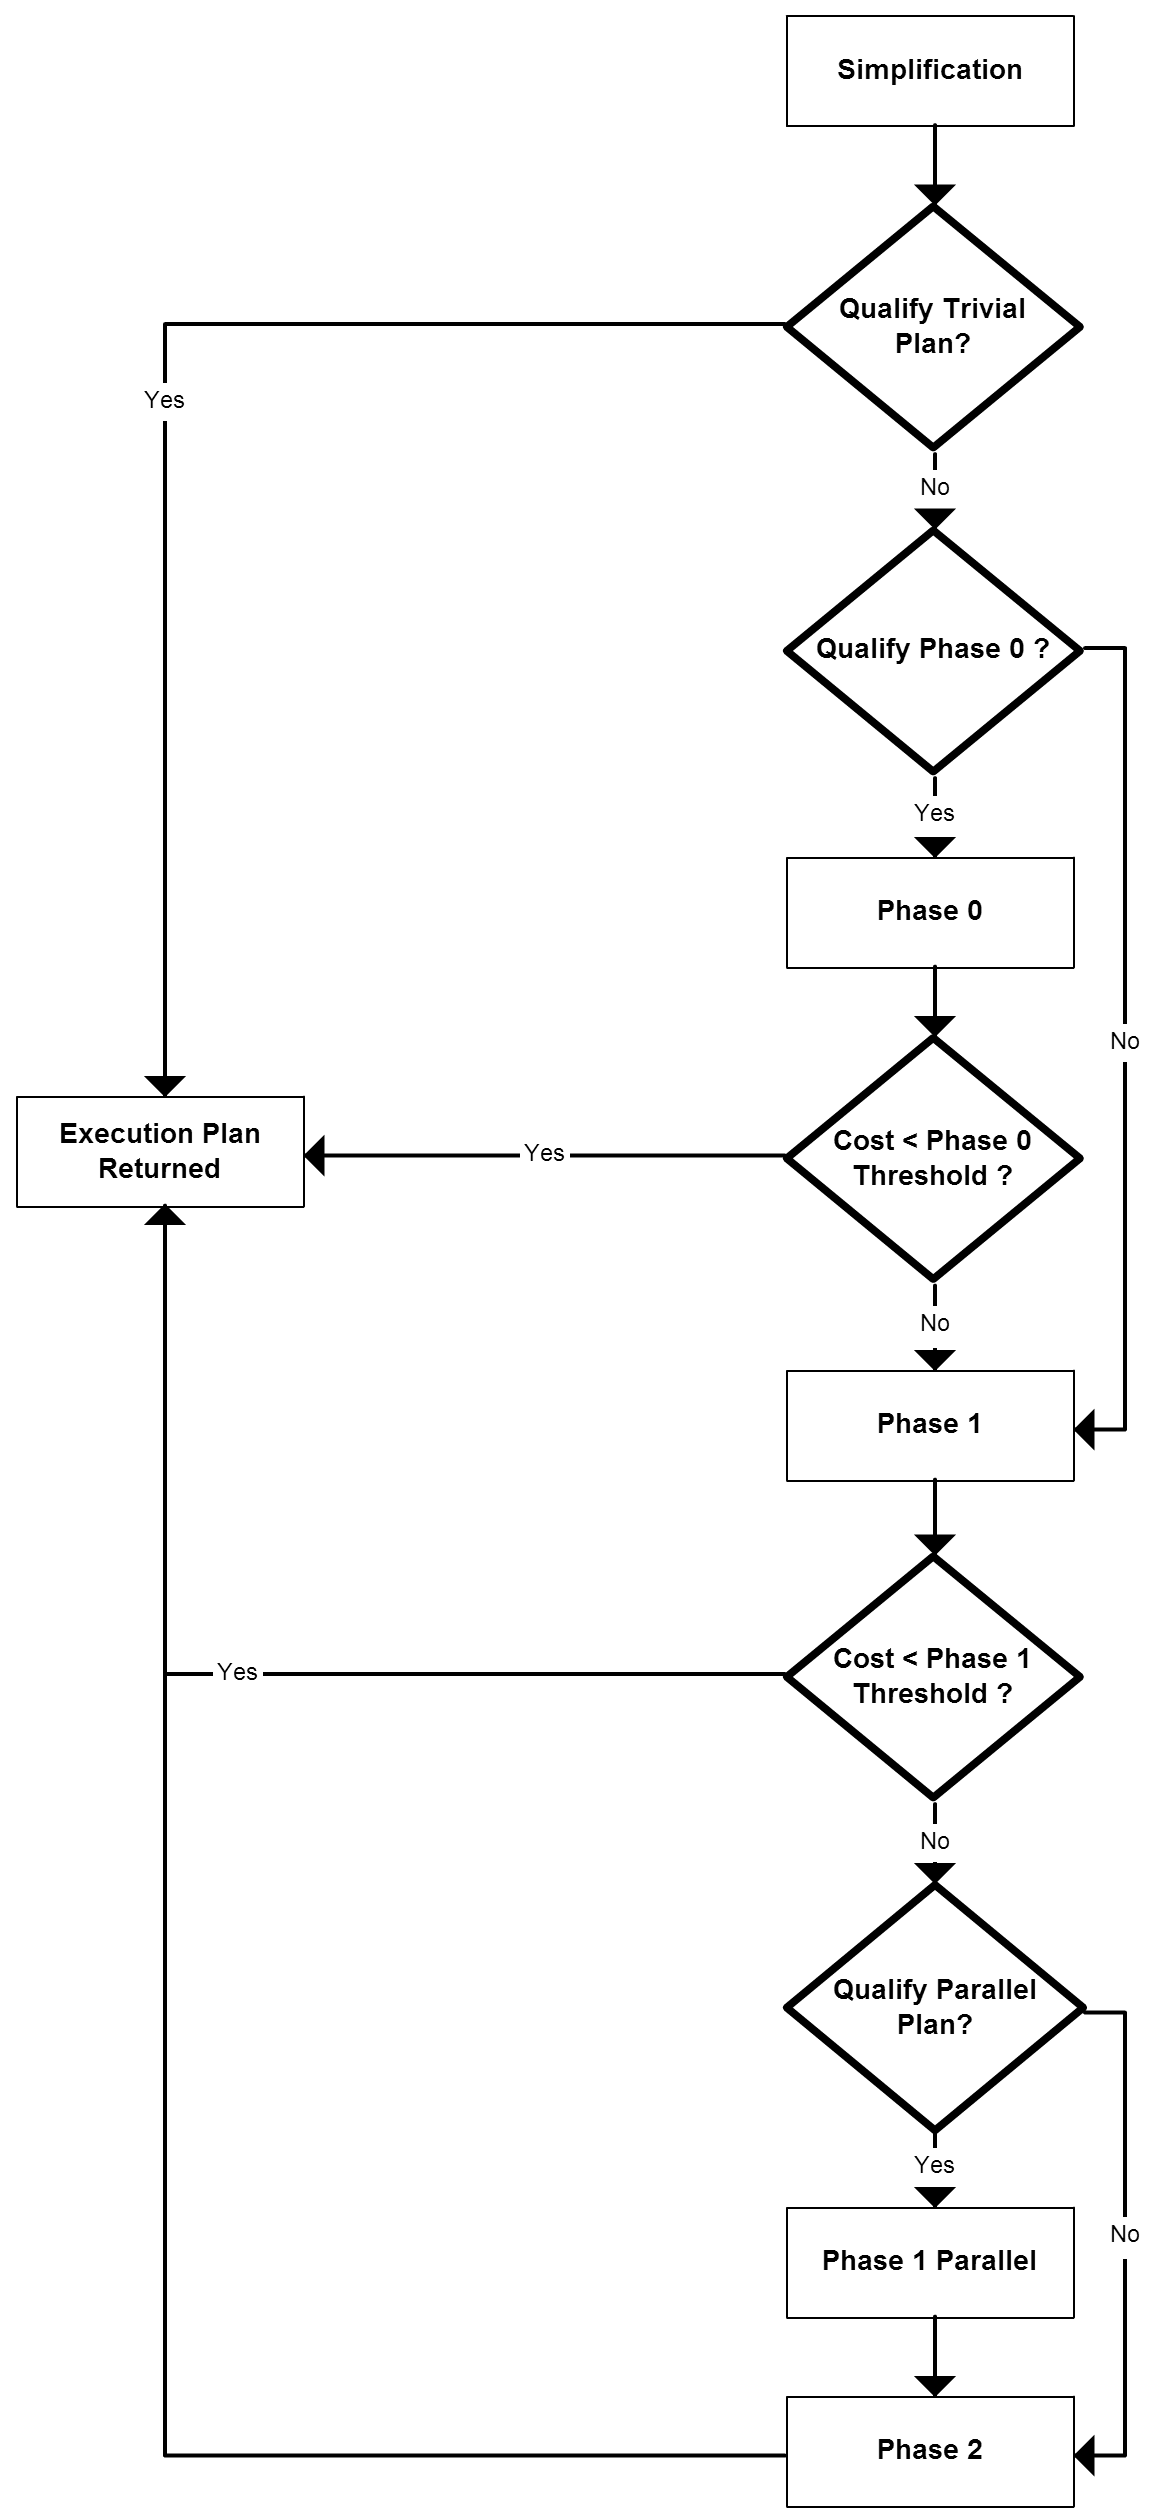
\includegraphics[scale=0.3]{Pictures/Optimization-process.png}
  \end{center}
  \vspace{-20pt}
  \caption{The query-processing process}
  \label{fig:qpp}
  \vspace{-10pt}
\end{figure}
\noindent As the query optimizer limits the available alternatives two problems arise. The entire search space is not evaluated and the chosen execution plan is therefore impossible to prove that it's the most optimal one. So the query optimizers utmost important functionality lies in considering the plans that are of low cost. Which brings us to another major technical challenge, accurate estimations. The quality of the plan that is chosen is only as good as the accuracy of the estimation. According to Nevarez    \cite{Nevarez} the estimations are inherently inexact and do not consider the environments hardware conditions. As an example the cost model assumes that every query's data is read from disk and not from memory (cold cache). In addition some operations are not covered by the mathematical model, leading to that the query optimizer has to resort to guessing logic and/or heuristics to deal with such situations. 

\subsubsection{Query tuning}
In order to optimize the process explained above there are numerous areas that can be altered. One can dive in to the actual SQL statements and try to break down complex queries, optimize join ordering etc. Besides altering the SQL statements the workload sent to the query optimizer can be optimized in several ways. Chaudhuri et al. \cite{compressing} state that compressing the size of a workload, which is a set of SQL statements, improves a systems scalability and illustrates its effectiveness in index selection and approximate query processing. Furthermore, major database vendors have focused on releasing automated physical database design tools that reduce the total cost of a workload. An essential assumption of these tools is that the workload consists of a set of SQL statements with no internal ordering. Agrawal et al. state that the workload in itself isn't the most promising aspect of workload optimization, but that the workload can be treated as a sequence which broadens the usage of the above mentioned tools, Agrawal et al. \cite{automatic}.

\paragraph*{Join ordering}\mbox{}\\\\
The order of joins is a key factor in controlling the amount of data flowing between operators in an execution plan. The query optimizer needs to pay close attention to this complex problem and has been the subject of extensive research since the 1970s  as mentioned in the study by Steinbrunn et al. \cite{join}. The task of the query optimizer is to find the optimal sequence of joins between tables in queries, and the way the joins are ordered can greatly impact the cost and performance of a query. Even though the result of query is the same, disregarding the join order, the cost can vary greatly. Joins have the properties of being both commutative and associative, because of these properties even simple queries can have many different possible join orders and increase exponentially with the number of tables that are involved. As mentioned earlier in section \ref{sec:qopt} the queries are represented as trees in the query processor. The shape of the tree is of utter importance for the query optimizer and is constructed by the nature of the join ordering. In table \ref{table:join} the number of possibilities depending on two sorts of tree shapes (seen in Figure \ref{fig:trees}) are listed, seemingly the number of possibilities increases dramatically. It's obviously impossible for the query optimizer to considere all these possibilities, it would take too long.  

\begin{figure}[H] 
\begin{center}
    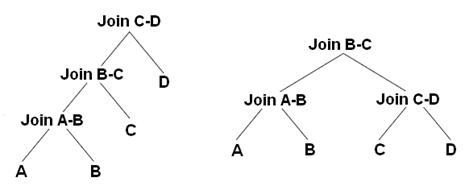
\includegraphics[scale=0.7]{Pictures/trees.jpg}
  \end{center}
  \caption{Left-deep and bushy trees}
  \label{fig:trees}
\end{figure} 
\begin{table}[H]
\centering 
\begin{tabular}{ l l l }
  Tables & Left-Deep Trees (n!) & Bushy Trees (2n-2)!/(n-1)! \\\hline
  2 & 2 & 2 \\\hline
  3 & 6 & 12 \\\hline
  4 & 24 & 120 \\\hline
  5 & 120 & 1 680 \\\hline
  6 & 720 & 30 240 \\\hline
  7 & 5 040 & 665 280 \\\hline
  8 & 40 320 & 17 297 280 \\\hline
  9 & 362 880 & 518 918 400 \\\hline
  10 & 3 628 800 & 17 643 225 600 \\\hline
  11 & 39 916 800 & 670 444 572 800 \\\hline
  12 & 479 001 600 & 28 158 588 057 600 \\
\end{tabular}
\caption {Possible join orders for Left-Deep and Bushy trees}
\label{table:join}
\end{table}

\noindent Since the number of the possibilities are that great the query optimizer needs to balance between the optimization time and the quality of it. So the goal of the query optimizer is to find a good enough plan as quick as possible. 

\paragraph*{Query break down}\mbox{}\\\\ \label{querybreakdown}
In some cases the query optimizer may not be able to produce/decide a good plan. This is mostly because of complex queries containing a large number of joins and joins with aggregations. Breaking down these complex queries into two or more and storing the intermediate result in temporary tables is a good plan, since it's fairly rare to request all the data in a single query. 
Howard   \cite{break-down} describes several problematic query patterns that the query optimizer has problems creating good plans for. The article is applied to SQL Server versions from 2005 to 2012 (code-named ''Denali''), but according to Nevarez \cite{Nevarez} it's also applicable to SQL Server 2014.\\ Two important query patterns for this thesis are:
\begin{itemize}
\item OR logic in Where clause
\item Joins on aggregated data sets
\end{itemize}

\subparagraph{\texttt{OR} logic in \texttt{WHERE} clause}\mbox{}\\\\
When the OR operator is evaluated on one and the same table, e.g. \texttt{WHERE a.col1=@val OR a.col2=@val2}, the query optimizer is able to create efficient execution plans by using index seek on two indexes and an index union. However if the \texttt{OR} operator is evaluated on different tables, e.g. \texttt{WHERE a.col1=@val OR b.col2=@val2}, poor plans may be created. Running the two following queries in Algorithm \ref{firstbreak-down} in Appendix \ref{appCode} will create two efficient plans.\\

\noindent If the two tables are joined using the same selective predicates as in Algorithm \ref{firstbreak-down} the SQL Server will return a very expensive plan. This can be fixed by using the \texttt{UNION} operator instead of the \texttt{OR} operator and allows for seeks on all indexes which results in a more efficient plan, even though the query looks more redundant and complex as seen in Algorithm \ref{second-down} in Appendix \ref{appCode}.


\subparagraph{Joins on aggregated data sets}\mbox{}\\\\
Most large queries join intermediate results from several query blocks involving grouping and aggregation. Earlier, aggregation meant grouping of a relation and then applying an aggregate function (e.g. average) on each group. This still applies, but companies and users are not interested in only e.g. the average salary of each employee. They want to do further grouping and sorting such as group the above mentioned employees based on their marital status and/or sex, Chatziantoniou \& Ross \cite{partioned}, consequently wanting to perform complex processing within each group and grouping among different sets of attributes.\\ A good cardinality estimation can be provided by statistics for operations performed on a table. However, queries using operators such as \texttt{GROUP} or \texttt{DISTINCT} create results with different number of rows than that are in the stored table. Joining these intermediate results on other data sets causes statistics on these intermediate results to not exist. If an intermediate result must be materialized before used in a subsequent step statistics are not available. The query optimizer tries to estimate the cardinality based upon the original data set, but since the earlier mentioned operators intermediate result differ from the original data set, the estimation can degrade in accuracy.\\\\ By analyzing the execution plan for these complex queries, one can partition the query where the estimated number of rows differ a lot from actual number of rows. To ensure statistics, one can store the intermediate results in temporary tables as mentioned in the beginning of this section.     

\subsection{Table partitioning} \label{sec:tablepart}
When the data in a database table grows massive in size it can become impractical to make \texttt{INSERT} and \texttt{DELETE} operations as well as maintaining proper indexes. The sheer size of the table can cause these operations to take much longer than practical standards.\\
Partitioning tables enables large tables and it indexes to become smaller portions of itself, the operations applied on the partitioned table can be applied on a partition-by-partition basis and the SQL Server optimizer can direct properly filtered queries on the intended partition instead of the entire table.\\
For SQL Servers there is mainly two different ways to partition tables; manually divide a large tables data into several physical tables or use the SQL Server's built in feature to partition a single table. The partitioning of data can be partitioned either horizontally or vertically, dividing the data and placed in different tables based on columns or rows respectively.\\For the manual way of table partitioning a view is often created that has bindings to the intended tables. This view acts as a superclass and the queries are directed to the view instead of the manually divided tables, creating what is called a \textit{partitioned view}. A big drawback of this manual partitioning is that the required constraints, indexing and operations need to be applied manually, consequently making maintenance possibly time-consuming and complex, Talmage \cite{tablepartitioning}. \\
Unlike the manual partitioning the built in feature does not include multiple physical tables. SQL Server automatically places the rows in the correct partition and maintains the partitions under the hood. Maintenance can be performed on individual partitions and properly filtered queries only access the correct partitions, the whole table does not need to be searched since partition elimination is performed.\\
The built in feature was introduced in SQL Server 2005 and since then every table in the database can be defined as partitioned. The tables are in fact a default partition consisting of one partition, itself, but is not truly a partitioned table without a partition scheme and a partition function as dependencies,as seen in Figure \ref{partdep}.
 
\tikzstyle{every node}=[draw=black,thick,anchor=west, fill=blue!10,style={draw,-latex}]
\begin{figure}[H]
\begin{center}
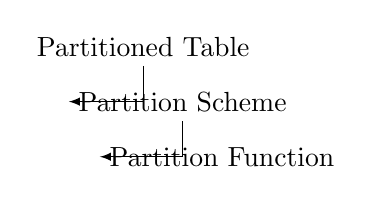
\begin{tikzpicture}[%
  grow via three points={one child at (0.5,-0.7) and
  two children at (0.5,-0.7) and (0.5,-1.4)},
  edge from parent path={(\tikzparentnode.south) |- (\tikzchildnode.west)},
  edge from parent/.style={draw,-latex}  
  ]
  \node {Partitioned Table}
    child { node {Partition Scheme}
		child {node {Partition Function}}    
    };
\end{tikzpicture}
\end{center}
\caption {Partitioned table dependencies}
\label{partdep}
\end{figure}
\noindent The table intended for partitioning must be created on a partition scheme that defines where the data is supposed to be stored, i.e. filegroup locations. The schema depends in turn on a partition function that determines the number of partitions and the data boundaries for the column that's intended as partition column in the table.
In Appendix \ref{appCode} in Algorithm \ref{partitionex}, Snaidero \cite{partitonexample} an example of making an already existing database table partitioned is shown by creating a partition scheme, a partition function and altering the tables constraints. Naturally if the partitioning is intended to be done on a non existing table, the constraints do not need to be dropped before creation. 
 
\subsection{In-Memory Database Technology}
Relational database management systems were originally designed in the late 70's, Nevarez \cite{Nevarez}. Because of this, they are designed with the assumption that memory is limited, expensive and that the size of the database is many times larger than the main memory. Today, memory is relatively cheap and it is possible to have hundreds of gigabytes of memory in a single server. This makes it possible to put even large databases, completely in memory. In Vizard's article   \cite{Vizard12} it is said that having a database completely in-memory can make it a thousand times faster.

\subsubsection{Hekaton}
Microsoft SQL Server 2014 comes with an In-Memory OLTP database engine called Hekaton. Hekaton, which is only available in the enterprise edition, improves performance in three major architecture areas: Optimization for main memory access, compiling procedures to native code, and latches and lock elimination. The core architecture of Hekaton is a Bw-tree design, Levandoski et al. \cite{Levandoski14}. A Bw-tree is a new design of the classical B-tree which supports high performance in both access to individual keys and key-sequential access to subranges of keys. The Bw-tree is designed for the new hardware environment in two main ways. 
\begin{enumerate}
\item The Bw-tree is latch-free, which is critical for performance when using multi-core systems where latches otherwise are common.
\item Updating cache memory in place in multi-core systems usually results in costly cache invalidations, limiting performance. By performing "delta" updates, the Bw-tree avoids in-place updates which reduces invalidations and preserves previously cached page data.
\end{enumerate} 
The Hekaton engine is not a separate database system, it is fully integrated into SQL Server. A user can declare a table in a current database to be memory-optimized, and the Hekaton engine will store it in main memory and manage it. A Hekaton table can use two different kinds of indexes. Hash indexes and Range indexes.  Even though Hekaton uses very different internal concepts and implementations it still ensures that all transactions have ACID-properties. ACID stands for atomicity, consistency, isolation and durability, Härder and Reuter \cite{haerder1983principles}. It's a set of properties that guarantees that database transactions are processed reliably. \\
A big drawback of using Hekaton tables is that the table architecture cannot be altered without recreating the table. This means that in order to change the columns in a table or its indexing settings, the table must be dropped and then rebuilt from scratch.

\paragraph*{Buckets}\mbox{}\\\\
The hash tables in Hekaton are implemented as regular hash tables with keys mapped via a hash function to values. The values are stored in an array of buckets, Barbarin \cite{Barbarin14}. \\\\
In Hekaton, the concept of buckets is an object that is reserved for the hash index when creating a memory optimized table. This parameter doesn't exist when discussing ordinary indexes or other special indexes. Microsoft recommends to select a bucket count of double the amount of distinct values in the table. The number of buckets also have to be a power of two and the parameter is static once set. This means that the table has to be dropped and rebuild if the bucket count is bad.

\begin{figure}[H]
\begin{center}
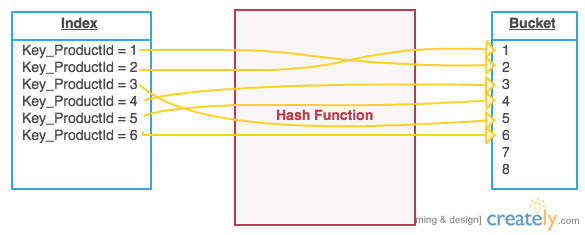
\includegraphics[scale=0.5]{Pictures/buckets.png}
\caption{Illustrating the concept of buckets}
\end{center}
\end{figure}

\noindent The hash indexes are in no particular order which makes it ineffective for range operations but fast for lookup operations. The hash function should be efficient enough to spread the keys into the buckets uniformly to avoid multiple values in the same bucket. Multiple values in the same bucket also occurs when there aren't enough buckets. This causes a bucket to have a row chain. This causes the lookup operation to be slower because it has to scan the row chain for the bucket to find the value. The number of keys per bucket is the \emph{load factor} of in-memory tables. This is calculated as the total number of entities divided by the number of buckets. The higher load factor, the slower a table will perform. This means that a fixed bucket count in a table will perform worse over time if the bucket count is too small. However, a too large bucket count will use excess memory and cause range lookups to perform slowly. 

\begin{figure}[H]
\begin{center}
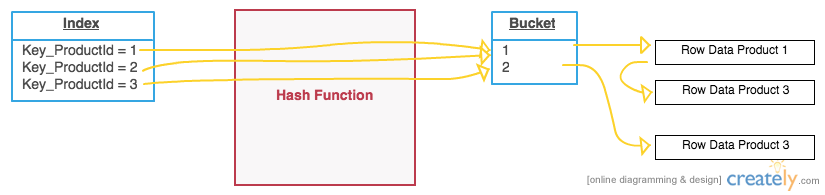
\includegraphics[scale=0.5]{Pictures/buckets2.png}
\caption{Illustrating the concept of a row chain}
\end{center}
\end{figure}

\noindent The reason why the bucket count has to be set as a power of two number is to make the hash function faster. The position for a value in a table is calculated as \emph{Hash value \% array size}. The problem with this calculation is that modulo is slow compared to the bit wise AND-operation. By setting the array size, which is the bucket count, to a number that is a power of two, one can use the AND-operation instead and save time.

\paragraph*{Stored procedures in Hekaton}\mbox{}\\\\ 
Hekaton uses the SQL Query Optimizer to produce an efficient query plan. This plane is then compiled into native C code and loaded as DLLs into the SQL Server process. This compilation happens on SQL Server start.
When a procedure is saved as a natively compiled stored procedure it locks all the tables that it uses. This is because such procedures must be schema bound, i.e. all tables referenced by a procedure can't be dropped. If this is considered together with the limitation mentioned above regarding changing of a table architecture, the following process would be required in order to change e.g. a Hekaton table's columns, Nevarez \cite{Nevarez}.
\begin{enumerate}
\item Drop the procedures referencing the table.
\item Store the data in the Hekaton in a temporary table.
\item Drop the Hekaton table.
\item Rebuild the Hekaton table with the new columns.
\item Reload the data from the temporary table into the new Hekaton table. 
\item Recreate the stored procedures.
\end{enumerate}

A complex procedure like this is preferably avoided. The cost of having to rebuild the in-memory tables from scratch could be high so it is important to plan and choose parameters wisely.


\section{Analysis}\label{sec:analysis}
The analysis of the system required several tools and environments for both live and local research, where the local environment setup is further explained in Appendix \ref{Aenviron}. To identify report-relevant parts of the system the tool Microsoft SQL Server Management Studio (SSMS) was mostly used. To identify and study the bottle-necks and problems, in the above mentioned system parts, several other tools such as DBVisualizer, SQL Sentry Plan Explorer etc. were used alongside SMSS to extract query duration, query execution plans and much more.\\\\
Much of the analysis revolved around the stored procedures, since it was there the potential of optimization was greatest, but other optimization areas were also studied such as index fragmentation of the relevant tables.      

\subsection{Stored procedures}\label{sec:sp}
As mentioned in the technical description a total of 59 stored procedures are present in the system. A little more than 50\% (30) of these subroutines are directly involved with the BI-reports. In the web interface there are several more reports that can be produced, but the ones not covered by stored procedures are treated in the back-end of the system.  
\begin{table}[H]
\begin{center}
\begin{tabular}{l p{9cm}}
Stored procedure: & Report(s)\\
1\_1\_1-1\_1\_9: & Sales $\rightarrow$ Standard\\
1\_2\_2: & Sales $\rightarrow$ Key Figures $\rightarrow$ Sales per weekday and hour \\
1\_3\_2: & Sales $\rightarrow$ Codes $\rightarrow$ Discount Codes  \\
1\_5\_1;1\_5\_2;1\_5\_7: & Sales $\rightarrow$ Order $\rightarrow$ Items; Variants; Daily Ordervalue\\
1\_6\_1: & Sales $\rightarrow$ Timesheets $\rightarrow$ Standard \\
2\_1\_1; 2\_1\_2: & Purchase $\rightarrow$ Standard $\rightarrow$ Items; Variants \\
2\_5; 2\_6: & Purchase $\rightarrow$ Purchase Planner $\rightarrow$ Rows; Advanced\\
3\_1-3\_7: & Location \\
4\_2-4\_5: & Accounting $\rightarrow$ Accounts, Dimension Matrix; Income Statement; Balance Sheet; Account, Day Matrix \\
\end{tabular}
\caption{The relation between stored procedures and BI-reports}
\end{center}
\end{table}

\noindent To execute the stored procedures, SQL batches such as Algorithm \ref{spexec} in Appendix \ref{appCode} were produced and executed. The SQL batches simply specifies the essential parameters and the optional ones as wildcards to get a wide range of data as possible.\\\\  
The stored procedures for BI-reports are quite similar considering the block of statements. The majority of the subroutines contain \texttt{SELECT}, \texttt{INSERT}, \texttt{UPDATE} and \texttt{DELETE} SQL block statements which differ in internal order and amount of statements. The \texttt{SELECT} statements vary greatly in the different stored procedure both in conditions and the tables they operate on. As can been seen in Table \ref{tab:tabfreq} in Appendix \ref{sec:appTabIll} the BI-report stored procedures work with a total of 82 tables and the average amount of dependencies for a stored procedure is approximately $\approx37$.\\
The data is fetched from the different tables by joining tables on stated conditions and then selected, at most, there is a stored procedure that has a total dependency of 46 different tables in its execution (see Table \ref{tab:mosttab} in Appendix \ref{sec:appTabIll}). The various stored procedures also have a resemblance as of from which tables the \texttt{JOIN}s are applied on. Table \ref{tab:tabfreq} in Appendix \ref{sec:appTabIll} shows that a total of 36 tables is the minimum amount of tables involved in all of the stored procedures.\\
The fetched data is stored as an intermediate result in a table with a name corresponding to the stored procedure name. This intermediate result table is present by reasons mentioned in \ref{querybreakdown}, with the exception that the table isn't temporary. The table is permanently present in the database due to a previously refactorization of the database by the DBA. The table is therefore meant as an optimization shortcut, where the last queried report result is stored until the same query is executed with different parameters.\\
The intermediate result table is then further altered by updates based on mathematical calculations such as item quantities, contribution margins etc. And in some cases a deletion is performed of rows where the mathematical calculations don't pass the set conditions such as if purchase-, sales- and/or stock-quantity is 0.   
       
\subsubsection{Execution statistics}
The first step taken to tune the stored procedure was to produce statistics. The goal of our thesis is to speed up the BI-report generation and thereby speeding up the stored procedures. Therefore execution duration was of utter importance and was established with the Transact-SQL \texttt{SET STATISTICS TIME} command, as can be seen in Algorithm \ref{spexec}. This command is used to measure variety of time, some of which may or may not be of much importance considering query tuning. The result varies from query to query and can look something like this: \\\\\texttt{SQL Server parse and compile time:\\
CPU time = 0 ms, elapsed time = 0 ms.\\
SQL Server parse and compile time:\\
CPU time = 0 ms,  elapsed time = 0 ms.\\
SQL Server Execution Times:\\
CPU time = 9002 ms,  elapsed time = 10634 ms.
}\\\\
To explain the above result we first need to clarify the two different measurements CPU-time and elapsed time. The CPU time is a relatively consistent measurement of the amount of CPU resources it takes for a query to run. This is obviously relatively independent of how busy the CPU is on the system the query is run. The elapsed time number is a measurement of how long the whole query took to execute (not including the time for locks or reads). This number is heavily dependent on the server load and can therefore change drastically according to McGehee \cite{statistics}. \\ In the above result example the first measurement block tells us how much time the SQL Server needed to parse, compile and put the execution plan in cache. The second measurement block tells us the amount of time it took the SQL Server to retrieve the execution plan from the cache. But what is most of interest is the third and frequently last measurement, it's the sum of all earlier measurements and therefore the measurement for the total duration of the query execution. This measurement will help us to determine if the future improvements actually were improvements considering execution speed.\\
The statistics measurements were taken on a system with a quad core processor as seen in Appendix \ref{Aenviron}. Because of this, the CPU-time will in some cases be greater than the elapsed time since the time stated in the result is then the sum of all busy processors' time. The parse and compile time were all the same for all stored procedures, 0ms, since the environment was established to simulate a live version as close as possible, meaning that almost every table, procedure and execution plan was present in the systems cache. But even though that almost everything was in the system cache, many of the stored procedures execution time were over a comfortable threshold, as can be seen in Table \ref{tab:duration}. 

\begin{table}[H]
\centering
\scalebox{0.9}{
\begin{tabular}{  l | l | l | l  H  H  H  H  H  }
	Stored procedure & \multicolumn{4}{c} {Local} &   Back-End &  & Live &  \\ \hline
	 & CPU (quad core) ms & CPU (single core) ms & elapsed ms & efficiency & CPU & elapsed & CPU & elapsed \\ \hline
	Report 2\_6 & 464372 & 116093 & 427017 & 0.271869738207144 &  &  &  & \  \\ \hline
	Report 2\_5 & 174594 & 43648.5 & 202116 & 0.2159576678738942 &  &  &  & \  \\ \hline
	Report 3\_1 & 138000 & 34500 & 147443 & 0.23398872784737151 &  &  &  & \  \\ \hline
	Report 4\_2 & 35187 & 8796.75 & 33168 & 0.26521798118668594 &  &  &  & \  \\ \hline
	Report 4\_4 & 29187 & 7296.75 & 39300 & 0.18566793893129771 &  &  &  & \  \\ \hline
	Report 1\_1\_2 & 18375 & 4593.75 & 21785 & 0.21086756942850585 &  &  &  & \  \\ \hline
	Report 1\_1\_1 & 9002 & 2250.5 & 10634 & 0.21163249952981003 &  &  &  & \  \\ \hline
	Report 1\_3\_2 & 8343 & 2085.75 & 9522 & 0.21904536862003782 &  &  &  & \  \\ \hline
	Report 4\_3 & 8046 & 2011.5 & 2536 & 0.79317823343848581 &  &  &  & \  \\ \hline
	Report 1\_1\_3 & 7860 & 1965 & 12655 & 0.15527459502173055 &  &  &  & \  \\ \hline
	Report 1\_1\_9 & 7687 & 1921.75 & 8998 & 0.2135752389419871 &  &  &  & \  \\ \hline
	Report 1\_1\_6 & 6813 & 1703.25 & 11381 & 0.14965732360952463 &  &  &  & \  \\ \hline
	Report 1\_1\_7 & 5968 & 1492 & 6429 & 0.23207341732773371 &  &  &  & \  \\ \hline
	Report 1\_1\_4 & 5937 & 1484.25 & 6347 & 0.23385063809673862 &  &  &  & \  \\ \hline
	Report 1\_1\_5 & 5860 & 1465 & 6249 & 0.23443751000160026 &  &  &  & \  \\ \hline
	Report 1\_1\_8 & 5344 & 1336 & 5973 & 0.22367319604888666 &  &  &  & \  \\ \hline
	Report 1\_2\_2 & 4452 & 1113 & 1244 & 0.89469453376205788 &  &  &  & \  \\ \hline
	Report 2\_1\_2 & 3125 & 781.25 & 3433 & 0.22757063792601223 &  &  &  & \  \\ \hline
	Report 1\_5\_7 & 3094 & 773.5 & 5483 & 0.14107240561736276 &  &  &  & \  \\ \hline
	Report 2\_1\_1 & 2360 & 590 & 2650 & 0.22264150943396227 &  &  &  & \  \\ \hline
	Report 4\_5 & 1217 & 304.25 & 3960 & 7.6830808080808083E-2 &  &  &  & \  \\ \hline
	
	\vdots & \vdots & \vdots & \vdots &  &  &  & \  
\end{tabular}}
\caption{Stored procedure execution duration on local database instance}
\label{tab:duration}
\end{table}

\noindent In the Table \ref{tab:duration} the most crucial stored procedures are listed, considering execution duration. As seen in section \ref{sec:BI} some of the critical reports are the ones that are troublesome time-wise.\\\\
The second Transact-SQL command that was used to produce useful statistics was \texttt{SET STATISTICS IO ON}, also seen in Algorithm \ref{spexec}.  The command provides detailed information about the query's impact on the SQL Server. An example of the output is shown below:\\\\
\texttt{Table 'HISTORY\_M'. Scan count 79508, logical reads 1632621, physical reads 0, read-ahead reads 0, lob logical reads 0, lob physical reads 0, lob read-ahead reads 0.}\\\\
Considering query tuning some of this information is helpful, and some not. The Scan count indicates how many times the referenced table was accessed. For queries including joins this information is quite helpful. The smaller the Scan count, the less resources needed and the better performance of the query. If the value is 0 it means that a unique index is used or a clustered index on a primary key. This information is good to keep an eye on when tuning the queries.\\ Logical reads is the most valuable information produced by the \texttt{SET STATISTICS IO ON} command, since it never changes from execution to execution on the same query and exact same data according to Richberg \cite{IO}. A logical read is the number of pages (see section \ref{sec:indexbad}) the SQL Server has to read from the cache to retrieve the result asked by the query. This is achieved due to the SQL Servers initial presence check, it checks if the pages it needs are in the data cache upon execution of a query. Fewer logical reads equals less resources used and hence better/faster performance, assuming all other things are held equal as prior to tuning.\\ When considering query tuning physical reads are often a discarded information. As mentioned above, the SQL Server checks if the needed data/pages are in the data cache, if not, the server needs to read the disk and store the information obtained in the data cache. The physical reads are dependent on the SQL Servers data cache and will diminish when executing the same query over and over again, so long there is enough room in the RAM. If this figure changes over time and/or execution, the changes can be caused due to memory pressure. The goal is of course to have a small figure as possible for this read, ergo having the needed pages in cache, ergo ensure that the physical RAM is plenty.\\ The Read-Ahead reads is directly tied to physical read and therefore not of interest to query tuning. SQL Server has a read-ahead mechanism that reads the physical data pages ahead, based on what the SQL server suspects is of interest, of when it's needed, Chaudhuri et al. \cite{readahead}. These pages may or may not be used, depending on the SQL Servers assumption. This information fluctuates, same as for physical reads, as pages are moved in/out of memory and can be affected by index fragmentation.\\ The large objects (LOB) logical-, physical- and read-ahead give respectively the same information as mentioned above but for large objects, data with the maximum size of 4 GB such as ASCII text, files in graphics formats etc. Ahmed et al. \cite{LOB}.  Since such data isn't present in the system, the importance of this information is out of this thesis scope.\\\\
The \texttt{SET STATISTICS IO ON} command, as for the \texttt{SET STATISTICS TIME ON} command, was executed on every stored procedure available in the system. Resulting in an output file of 300 lines of text. This was of course not manageable to analyze and read, so with the help of Vicky Harts excel template    \cite{Vicky} and Richie Rumps Statistics Parser web application    \cite{Rump}, an Excel worksheet was developed (with a few alterations and improvements). In Table \ref{tab:IO} a fraction of the output is listed. Even here the most critical reports top the list for IO statistics. The total sum of pages read logical is $\approx$ 4.7$\times 10^9$ pages for all stored procedure. In Table {tab:IO} the LOB information is cut out due to nonexistence of LOB's in the system.\\ Only a total of 9956 pages were read from disk, meaning that a lot of the necessary data is present in the SQL Servers data cache. The anomalies should be the result of full memory and the system therefore priorities what should be in cache. 
\begin{table}[H]
\centering
\scalebox{0.8}{
\begin{tabular}{  l | H  l | l | l | l | l  H H H }

	Stored procedure &  & Object name & Scan count & Logical reads & Physical reads & Read-Ahead Reads & Lob Logical Reads & Lob Physical Reads & Lob read-ahead reads  \  \\ \hline
	3\_1 & Table ' SALES\_H'. Scan count 0, logical reads 68850420, physical reads 0, read-ahead reads 0, lob logical reads 0, lob physical reads 0, lob read-ahead reads 0. &  SALES\_H & 0 & 68850420 & 0 & 0 & 0 & 0 & 0 \\ \hline
	2\_6 & Table 'Worktable'. Scan count 1589989, logical reads 49956351, physical reads 0, read-ahead reads 0, lob logical reads 0, lob physical reads 0, lob read-ahead reads 0. & Worktable & 1589989 & 49956351 & 0 & 0 & 0 & 0 & 0 \\ \hline
	2\_6 & Table 'Worktable'. Scan count 1589989, logical reads 47508411, physical reads 0, read-ahead reads 0, lob logical reads 0, lob physical reads 0, lob read-ahead reads 0. & Worktable & 1589989 & 47508411 & 0 & 0 & 0 & 0 & 0 \\ \hline
	2\_5 & Table 'Worktable'. Scan count 1318326, logical reads 46380365, physical reads 0, read-ahead reads 0, lob logical reads 0, lob physical reads 0, lob read-ahead reads 0. & Worktable & 1318326 & 46380365 & 0 & 0 & 0 & 0 & 0 \\ \hline
	2\_6 & Table 'Worktable'. Scan count 370813, logical reads 40890291, physical reads 0, read-ahead reads 0, lob logical reads 0, lob physical reads 0, lob read-ahead reads 0. & Worktable & 370813 & 40890291 & 0 & 0 & 0 & 0 & 0 \\ \hline
	2\_5 & Table ' HISTORY\_M'. Scan count 2257991, logical reads 20336741, physical reads 241, read-ahead reads 27358, lob logical reads 0, lob physical reads 0, lob read-ahead reads 0. &  HISTORY\_M & 2257991 & 20336741 & 241 & 27358 & 0 & 0 & 0 \\ \hline
	4\_2 & Table ' HISTORY\_M'. Scan count 9, logical reads 15318541, physical reads 1940, read-ahead reads 167916, lob logical reads 0, lob physical reads 0, lob read-ahead reads 0. &  HISTORY\_M & 9 & 15318541 & 1940 & 167916 & 0 & 0 & 0 \\ \hline
	3\_1 & Table 'Worktable'. Scan count 1116354, logical reads 13974108, physical reads 0, read-ahead reads 0, lob logical reads 0, lob physical reads 0, lob read-ahead reads 0. & Worktable & 1116354 & 13974108 & 0 & 0 & 0 & 0 & 0 \\ \hline
	2\_6 & Table ' HISTORY\_M'. Scan count 370836, logical reads 13801901, physical reads 1184, read-ahead reads 177558, lob logical reads 0, lob physical reads 0, lob read-ahead reads 0. &  HISTORY\_M & 370836 & 13801901 & 1184 & 177558 & 0 & 0 & 0 \\ \hline
	2\_6 & Table ' ITEM\_L\_E'. Scan count 1589989, logical reads 11407484, physical reads 0, read-ahead reads 0, lob logical reads 0, lob physical reads 0, lob read-ahead reads 0. &  ITEM\_L\_E & 1589989 & 11407484 & 0 & 0 & 0 & 0 & 0 \\ \hline
	2\_6 & Table ' SALES\_H'. Scan count 5307607, logical reads 10645764, physical reads 0, read-ahead reads 0, lob logical reads 0, lob physical reads 0, lob read-ahead reads 0. &  SALES\_H & 5307607 & 10645764 & 0 & 0 & 0 & 0 & 0 \\ \hline
	3\_1 & Table 'Worktable'. Scan count 2232708, logical reads 10205255, physical reads 0, read-ahead reads 0, lob logical reads 0, lob physical reads 0, lob read-ahead reads 0. & Worktable & 2232708 & 10205255 & 0 & 0 & 0 & 0 & 0 \\ \hline
	2\_5 & Table ' SALES\_H'. Scan count 4868901, logical reads 9765541, physical reads 0, read-ahead reads 0, lob logical reads 0, lob physical reads 0, lob read-ahead reads 0. &  SALES\_H & 4868901 & 9765541 & 0 & 0 & 0 & 0 & 0 \\ \hline
	2\_5 & Table ' ITEM\_L\_E'. Scan count 1318326, logical reads 9644543, physical reads 0, read-ahead reads 4, lob logical reads 0, lob physical reads 0, lob read-ahead reads 0. &  ITEM\_L\_E & 1318326 & 9644543 & 0 & 4 & 0 & 0 & 0 \\ \hline
	2\_6 & Table 'Worktable'. Scan count 1589989, logical reads 8500919, physical reads 0, read-ahead reads 0, lob logical reads 0, lob physical reads 0, lob read-ahead reads 0. & Worktable & 1589989 & 8500919 & 0 & 0 & 0 & 0 & 0 \\ \hline
	2\_5 & Table 'Worktable'. Scan count 1318326, logical reads 7530165, physical reads 0, read-ahead reads 0, lob logical reads 0, lob physical reads 0, lob read-ahead reads 0. & Worktable & 1318326 & 7530165 & 0 & 0 & 0 & 0 & 0 \\ \hline
	3\_1 & Table ' PURCHASE\_H'. Scan count 0, logical reads 5453698, physical reads 0, read-ahead reads 0, lob logical reads 0, lob physical reads 0, lob read-ahead reads 0. &  PURCHASE\_H & 0 & 5453698 & 0 & 0 & 0 & 0 & 0 \\ \hline
	2\_6 & Table ' REPORT\_RESULT\_2\_6'. Scan count 1, logical reads 4950883, physical reads 0, read-ahead reads 0, lob logical reads 0, lob physical reads 0, lob read-ahead reads 0. &  REPORT\_RESULT\_2\_6 & 1 & 4950883 & 0 & 0 & 0 & 0 & 0 \\ \hline
	2\_5 & Table ' REPORT\_RESULT\_2\_5'. Scan count 1, logical reads 4116135, physical reads 0, read-ahead reads 0, lob logical reads 0, lob physical reads 0, lob read-ahead reads 0. &  REPORT\_RESULT\_2\_5 & 1 & 4116135 & 0 & 0 & 0 & 0 & 0 \\ \hline
	1\_1\_2 & Table ' REPORT\_RESULT\_1\_1\_2'. Scan count 1, logical reads 3811767, physical reads 65, read-ahead reads 63, lob logical reads 0, lob physical reads 0, lob read-ahead reads 0. &  REPORT\_RESULT\_1\_1\_2 & 1 & 3811767 & 65 & 63 & 0 & 0 & 0 \\ \hline
	1\_5\_7 & Table ' SALES\_H'. Scan count 0, logical reads 2117142, physical reads 0, read-ahead reads 0, lob logical reads 0, lob physical reads 0, lob read-ahead reads 0. &  SALES\_H & 0 & 2117142 & 0 & 0 & 0 & 0 & 0 \\ \hline
	 1\_1\_1 & Table ' HISTORY\_M'. Scan count 79508, logical reads 1632621, physical reads 0, read-ahead reads 0, lob logical reads 0, lob physical reads 0, lob read-ahead reads 0. &  HISTORY\_M & 79508 & 1632621 & 0 & 0 & 0 & 0 & 0 \\ \hline
	1\_1\_2 & Table ' HISTORY\_M'. Scan count 79508, logical reads 1632621, physical reads 0, read-ahead reads 0, lob logical reads 0, lob physical reads 0, lob read-ahead reads 0. &  HISTORY\_M & 79508 & 1632621 & 0 & 0 & 0 & 0 & 0 \\ \hline
	1\_1\_3 & Table ' HISTORY\_M'. Scan count 79508, logical reads 1632621, physical reads 0, read-ahead reads 0, lob logical reads 0, lob physical reads 0, lob read-ahead reads 0. &  HISTORY\_M & 79508 & 1632621 & 0 & 0 & 0 & 0 & 0 \\ \hline
	1\_1\_4 & Table ' HISTORY\_M'. Scan count 79508, logical reads 1632621, physical reads 0, read-ahead reads 0, lob logical reads 0, lob physical reads 0, lob read-ahead reads 0. &  HISTORY\_M & 79508 & 1632621 & 0 & 0 & 0 & 0 & 0 \\ \hline
	1\_1\_5 & Table ' HISTORY\_M'. Scan count 79508, logical reads 1632621, physical reads 0, read-ahead reads 0, lob logical reads 0, lob physical reads 0, lob read-ahead reads 0. &  HISTORY\_M & 79508 & 1632621 & 0 & 0 & 0 & 0 & 0 \\ \hline
	1\_1\_6 & Table ' HISTORY\_M'. Scan count 79508, logical reads 1632621, physical reads 0, read-ahead reads 0, lob logical reads 0, lob physical reads 0, lob read-ahead reads 0. &  HISTORY\_M & 79508 & 1632621 & 0 & 0 & 0 & 0 & 0 \\ \hline
	1\_1\_7 & Table ' HISTORY\_M'. Scan count 79508, logical reads 1632621, physical reads 0, read-ahead reads 0, lob logical reads 0, lob physical reads 0, lob read-ahead reads 0. &  HISTORY\_M & 79508 & 1632621 & 0 & 0 & 0 & 0 & 0 \\ \hline
	1\_1\_8 & Table ' HISTORY\_M'. Scan count 79508, logical reads 1632621, physical reads 0, read-ahead reads 0, lob logical reads 0, lob physical reads 0, lob read-ahead reads 0. &  HISTORY\_M & 79508 & 1632621 & 0 & 0 & 0 & 0 & 0 \\ \hline
	1\_1\_9 & Table ' HISTORY\_M'. Scan count 79508, logical reads 1632621, physical reads 0, read-ahead reads 0, lob logical reads 0, lob physical reads 0, lob read-ahead reads 0. &  HISTORY\_M & 79508 & 1632621 & 0 & 0 & 0 & 0 & 0 \\ \hline
	1\_3\_2 & Table ' HISTORY\_M'. Scan count 79508, logical reads 1632621, physical reads 0, read-ahead reads 0, lob logical reads 0, lob physical reads 0, lob read-ahead reads 0. &  HISTORY\_M & 79508 & 1632621 & 0 & 0 & 0 & 0 & 0 \\ \hline
	1\_3\_2 & Table ' HISTORY\_M'. Scan count 79508, logical reads 1632621, physical reads 0, read-ahead reads 0, lob logical reads 0, lob physical reads 0, lob read-ahead reads 0. &  HISTORY\_M & 79508 & 1632621 & 0 & 0 & 0 & 0 & 0 \\ \hline
	1\_2\_2 & Table ' HISTORY\_M'. Scan count 9, logical reads 1445404, physical reads 0, read-ahead reads 0, lob logical reads 0, lob physical reads 0, lob read-ahead reads 0. &  HISTORY\_M & 9 & 1445404 & 0 & 0 & 0 & 0 & 0 \\ \hline
	2\_5 & Table ' ITEM\_L\_E'. Scan count 234290, logical reads 1242358, physical reads 0, read-ahead reads 437, lob logical reads 0, lob physical reads 0, lob read-ahead reads 0. &  ITEM\_L\_E & 234290 & 1242358 & 0 & 437 & 0 & 0 & 0 \\ \hline
	2\_6 & Table ' REPORT\_RESULT\_2\_6'. Scan count 0, logical reads 1235223, physical reads 0, read-ahead reads 0, lob logical reads 0, lob physical reads 0, lob read-ahead reads 0. &  REPORT\_RESULT\_2\_6 & 0 & 1235223 & 0 & 0 & 0 & 0 & 0 \\ \hline
	\vdots & \vdots & \vdots & \vdots & \vdots  & \vdots & \vdots & \vdots\ & \vdots & \vdots 
\end{tabular}}
\caption{The top part, sorted by logical reads, of stored procedure execution IO statistics}
\label{tab:IO}
\end{table}
\noindent The above information is part of the key information to tuning the stored procedures, especially the Scan count and Logical reads. But to properly alter the key item we need to use the information in conjunction with the queries execution plans, Richberg \cite{IO}.  

\subsubsection{Execution plans}
An execution plan is an algorithm calculated by the SQL Servers Query Optimizer using the minimum of the server's resources. It shows the necessary set of steps in a specific order that is executed to obtain the data access in a database. The execution plans corresponding to the stored procedures in the system were obtained in a graphical perspective through SMSS. These execution plans contain graphical representations of operations, operation costs, operation properties and values as well as helpful warnings. The variety of operations and their properties are too cumbersome to explain in detail in writing. Therefore this sections focal point will be summarizing the execution plans corresponding to the most critical stored procedure and one in particular as an example.\\\\      
With the help of SQL Sentry Plan Explorer the execution plans could be further analyzed. As execution plans tend to accommodate a lot of information it's problematic to quickly identify operations or signs that are troublesome and can be improved. According to Fritchey \cite{fritchey2} there are a few common signs of trouble:
\begin{table}[H]
\begin{center}
\begin{tabular}{p{3cm} p{10cm}}
Warnings & Indicates such as missing indexes or conversion problems\\
Costly operations & An indication of where to start troubleshooting.\\ & Not an actual measure, estimated value.\\
Fat pipes & Indication of a lot of data being processed, which sometimes is inevitable, but transitions between fat and thin pipes indicate of late filtering and can be a problem.\\
Extra operations & Operations that are present for unintended reasons by the developer but are present due to e.g. the SQL Query Optimizer, are a potential problem\\
Scans & Often an indication of bad filtering or indexing, not necessarily a bad thing if an index scan is intended\\
Actual \# rows vs. estimated \# rows & Indication of cardinality estimate issues\\
\end{tabular}
\end{center}
\end{table}
 
Table \ref{2_5 overview} and Figure \ref{2_5 ep} below represent the execution plan for stored procedure 2\_5.
\begin{table}[H]
\centering
\resizebox{\linewidth}{!}{
\begin{tabular}{|p{3,3cm}|l|l|l|l|l|l|}
\hline
Statement & Est. Cost & Est. CPU & Est. I/O Cost & Est. Rows & Actual Rows & Key Lookups\\\hline
insert into  Table X &	0,0\% & 0,0\% & 0,0\% & \cellcolor{red} 7 & \cellcolor{red} 235 270 & 2\\\hline 
update  Table X set PurchaseQty & 55,5\% & 93,6\% & 44,5\% & 651 830 & 651 830 & 0 \\\hline 
update  Table X set StockQty & 17,6\% & 0,0\% & 25,3\% & 651 830 & 651 830 & 0 \\\hline 
update  Table X set AvailableQty & 20,3\% & 6,4\% & 16,5\% & 651 830 & 651 830 & 0 \\\hline 
delete from  Table X & 0,0\% & 0,0\% & 0,0\% &\cellcolor{red} 1 & \cellcolor{red} 151 958& 0 \\\hline 
update  Table X set TBPercent & 6,6\% & 0,0\% & 13,6\% & 499 872 &  499 872 & 0 \\\hline 
\end{tabular}}
\caption{Overview of stored procedure 2\_5's statement blocks in execution plan}
\label{2_5 overview}
\end{table}

\noindent As mentioned earlier almost every stored procedure contain similar statement blocks such as \texttt{INSERT, UPDATE, DELETE}. The estimated cost and operation percentages shown in an execution plan are not directly correlated with time, they show a relative calculated internal estimation of resources used by the batch and operations, Watson \cite{cost}. High percentage values don't necessarily mean it's bad, but is often an indication of room for improvement. Since the estimated cost is an internal relative estimation, it's not a good measurement to compare queries with. Contrariwise the CPU cost and I/O are solid comparative signs. 
\begin{wrapfigure}{r}{0.35\textwidth}
  \vspace{-20pt}
  \begin{center}
    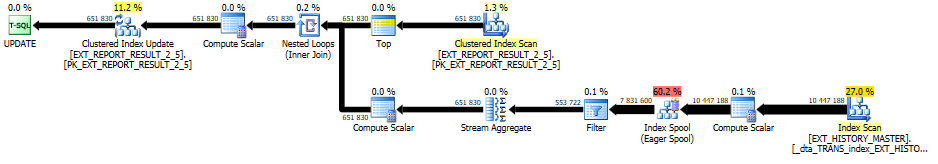
\includegraphics[scale=0.8]{Pictures/plan.png}
  \end{center}
  \vspace{-20pt}
  \caption{Graphical execution plan of the most resource-intensive \texttt{UPDATE} statement in stored procedure 2\_5}
  \label{2_5 ep}
  \vspace{-40pt}
\end{wrapfigure}
In Table \ref{2_5 overview} the first \texttt{UPDATE} statement is the villain in stored procedure 2\_5. Which is clarified by the CPU cost and the relative statement cost compared to the other statements in the SQL batch. We can also see from the overview above that cardinality estimate issues may be in place in the \texttt{INSERT} and \texttt{DELETE} statements, due to the huge skew in the comparison between actual number of rows and estimated number of rows.\\\\    
In figure \ref{2_5 ep} the graphical execution plan for the most resource-intensive \texttt{UPDATE} statement in stored procedure 2\_5 is shown. The execution plan is read from bottom to top and left to right. The operation costs all add up to 100\% since the costs are a relative sum of the CPU and I/0 costs. The execution plan starts with an Index scan on the HISTORY\_M table and returns all of the entries in the table belonging to a specific user ID. The \texttt{UPDATE} statement makes a calculation on every entity to be able to update the quantity of the sold articles. Since the entities in HISTORY\_M are not in any specific order the scan needs to be of the entire table to group and calculate a sum of all unique entries (the Compute scalar operation at the bottom represents a negative application on the articles quantity). This is of course not optimal in any way, but for this query sadly inevitable. According to Fritchey \cite{fritchey} an Index scan is quite common and occurs if the query optimizer determines that it's quicker to scan all the values in the entire index than to use the key provided by the index, since so many rows need to be returned. To reduce the returned rows a fine-tuning in the \texttt{WHERE}-clause has to be done. \\\\ 
The next operator is an Index Spool. This operator stores each of the rows to be updated and creates a temporary index, which is then used instead of the original table indexes. Without this operations every article update would initiate the earlier mentioned Index scan. Instead the spooled data can be reused later if the operator is rewound. In the stored procedure this operation is actually rewound 651 830 times due to number of entities in the result table. This is better than redoing the Index scan 651 830 times, but still very suboptimal. The rewinding is caused in conjunction with the Clustered Index Scan on the result table and the nested loop that compares the entities in HISTORY\_M, meaning a rewind for every comparison/row in the result table. The output of the Index Spool is filtered based on the predicates stated in the \texttt{WHERE}-clause. The filtered output is then calculated on a certain predicate through a Stream Aggregate, the Stream Aggregate   is used to group some rows and to calculate a big aggregated expression. According to Amorim \cite{streamaggregate} The Stream Aggregates' output is a BigInt value and is the reason for the following Compute Scalar operation, it converts the BigInt value to an Integer data type. The Compute Scalar conversion can be avoided if the query is altered, but there is no gain in performance improvement since the Compute Scalar conversion takes 0.0\% of the CPU. \\\\
It's not until the penultimate operation (Clustered Index Update) the rows identification is done and the actual update is done. The operator at the top in figure \ref{2_5 ep} is a T-SQL Language Element Catchall operator, which tells us, in this case, that an \texttt{UPDATE} operation has been completed. This operator also indicates that a minor problem existed, a warning label in the form of a yellow triangle. This warning tells us that there is a missing index on the result table and by creating one the performance could be improved.\\\\
This warning, among others, is the most common in the current system. According to estimates by SQL Sentry Plan Explorer some \texttt{UPDATE} statements in the stored procedures can be performance improved up to 70,5 \% by implementing these missing indexes. But it also gives the warning that this estimate is based solely upon analysis of that specific query and has not taken the external factors, such as the resulting index size or its workload-wide impact, in to account.\\\\ 
Other common warnings that were encountered were "spill to temp database" and "convert issues". The "spill to temp database" issue is due to bad cardinality estimates. The SQL Server allocates memory before execution and is therefore dependent on the estimated number of rows. If a sort operation receives more rows than it estimated (more actual rows than estimated rows) more memory is needed and therefore data is spilled/read to/from disk, Radivojevic \cite{sortissues}. The "convert issues" is caused when data is implicitly or explicitly converted to another data type. This is performed on the data in the table columns, resulting in altering the conceivable present index on that column. Causing the SQL server to ignore that index and perform a table scan since the index implementation doesn't coincide with the data, Fritchey \cite{convertissues}.\\\\
Through the analysis of the execution plans many trouble signs were noted. Except for the warnings in several execution plans, cardinality estimates seems to be a big issue where estimated rows substantially differ from actual rows. As for operations Clustered Index Scan and Clustered Index Update are most definitely the most common operation throughout the stored procedures. Indicating that the indexes present on the database tables in the system are not optimal and should be revised.    

\newpage
\subsection{Index fragmentation}\label{indexfragmentation}
By using the script from the theory the following index fragmentation values in Table \ref{indexfrag} were produced. The table names and index names has been shortened and/or changed due to confidentiality.
\begin{center}
\begin{table}[H]
\scalebox{0.92}{
\begin{tabular}{|l|l|l|l|}
\hline
Table Name         & Index Name                & Ext. Frag. & Int. Frag.\\ \hline
COMPILED\_ST       & IX\_COMPILED\_ST\_2       & 100                    & 74,05485545            \\ \hline
COMPILED\_ST       & IX\_COMPILED\_ST\_1       & 100                    & 72,6278725             \\ \hline
CUSTOMER\_B\_L\_E  & IX\_CUSTOMER\_B\_L\_E     & 100                    & 58,68544601            \\ \hline
CUSTOMER           & PK\_CUSTOMER\_1           & 100                    & 70,17500618            \\ \hline
CUSTOMER           & \_POSANA\_dta\_i\_C       & 100                    & 67,92068199            \\ \hline
SALES\_H           & \_REST\_dta\_index\_S\_H  & 100                    & 58,46971831            \\ \hline
SALES\_H           & \_dta\_index\_S\_H\_      & 100                    & 50,03706449            \\ \hline
CUSTOMER           & PK\_C\_1                  & 99,48535234            & 57,89085743            \\ \hline
SALES\_I\_H        & PK\_SALES\_I\_H           & 96,11111111            & 73,69038794            \\ \hline
SALES\_CR\_M\_H    & \_dta\_index\_S\_CR\_M\_H & 94,44444444            & 70,63737336            \\ \hline
CUSTOMER           & \_POSANA\_dta\_i\_C       & 90,59325223            & 52,81183593            \\ \hline
HISTORY\_M         & PK\_HISTORY\_M            & 89,13043478            & 65,47550037            \\ \hline
SALES\_I\_H        & \_dta\_index\_S\_I\_H     & 86,99186992            & 65,83502595            \\ \hline
SUPPLIER           & PK\_SUPPLIER\_1           & 85,71428571            & 47,9579318             \\ \hline
CUSTOMER           & \_POSANA\_dta\_i\_C       & 78,98550725            & 57,05273042            \\ \hline
SALES\_H           & \_dta\_index\_S\_H\_S     & 77,77777778            & 56,54531752            \\ \hline
REPORT\_R\_1\_1\_1 & IX\_REPORT\_R             & 76,57657658            & 39,54536694            \\ \hline
REPORT\_R\_4\_4    & PK\_REPORT\_R\_4\_4       & 75                     & 69,08512478            \\ \hline
SALESPERSON        & PK\_SALESPERSON           & 75                     & 48,44946874            \\ \hline
SALES\_CR\_M\_H    & PK\_SALES\_CR\_M\_H       & 73,35790885            & 62,85373116            \\ \hline
SALES\_CR\_M\_H    & \_dta\_index\_S\_CR\_M\_H & 71,30559541            & 64,10468248            \\ \hline
HISTORY\_M         & PK\_HISTORY\_M            & 69,67213115            & 69,75221151            \\ \hline
SALES\_I\_H        & \_dta\_index\_S\_I\_H     & 68,46173667            & 65,69195701            \\ \hline
SALES\_I\_H        & PK\_SALES\_I\_H           & 67,79506955            & 65,90287868            \\ \hline
HISTORY\_M         & \_dta\_TRANS\_i\_H\_M     & 66,66666667            & 49,09809736            \\ \hline
REPORT\_R\_1\_1\_1 & IX\_REPORT\_R\_1\_1\_1\_2 & 63,55140187            & 41,02462318            \\ \hline
REPORT\_R\_1\_1\_2 & IX\_REPORT\_R\_1\_1\_2\_3 & 60,68376068            & 43,8769706             \\ \hline
COUNTRY            & PK\_COUNTRY\_1            & 50                     & 53,43464295            \\ \hline
REPORT\_R\_1\_1\_5 & PK\_REPORT\_R\_1\_5       & 50                     & 66,04274771            \\ \hline
ITEM\_I            & PK\_ITEM\_I               & 50                     & 54,92957746            \\ \hline
PROGRAM            & PK\_PROGRAM\_1            & 50                     & 74,49962936            \\ \hline
CUSTOMER           & IX\_C\_1                  & 50                     & 41,83552014            \\ \hline
REPORT\_R\_2\_1\_1 & PK\_REPORT\_R\_2\_1\_1    & 50                     & 51,23754633            \\ \hline
REPORT\_R\_1\_1\_2 & IX\_REPORT\_R\_1\_1\_2\_2 & 47,68041237            & 52,92886088            \\ \hline
SALES\_H           & PK\_SALES\_H              & 36,59652333            & 72,06630838            \\ \hline
SALES\_H           & \_dta\_index\_S\_H\_M1    & 33,5729147             & 73,20072894            \\ \hline
REPORT\_R\_3\_1    & PK\_REPORT\_R\_3\_1       & 29,51672862            & 28,8227576             \\ \hline
REPORT\_R\_2\_6    & PK\_REPORT\_2\_6          & 18,96085152            & 44,27150976            \\ \hline
REPORT\_R\_2\_5    & PK\_REPORT\_R\_2\_5       & 14,15848367            & 45,84052384            \\ \hline
REPORT\_R\_3\_1    & PK\_REPORT\_R\_3\_1       & 10,71428571            & 7,690449716            \\ \hline
\end{tabular}}
\caption{Table showing all the fragmented indexes}
\label{indexfrag}
\end{table}
\end{center}
This shows that 40 out of 572 indexes have both internal and external fragmentation. Some of the indexes used have an external fragmentation well above the value of 10, which is the threshold according to Shubho \cite{Shubho09} as mentioned in section \ref{measurefrag}. The internal fragmentation value is also bad at some of the indexes (i.e. less than 75). This shows that BeX Online over time gives rise to fragmented indexes which has to be taken care of. The indexes with heavy fragmentation are used in tables that are the most frequently used by the stored procedures to create business intelligence reports. This fragmentation is most likely a reason to poor performance in these queries.

\subsection{Table experimentation} \label{Experiments}
With the help of the above analysis some experimentation of the BI-stakeholder tables were performed. The goal of this was to both identify the parts that were problematic in the stored procedures and see if table partitioning is a feasible solution.
With the help of earlier statistics, in collaboration with what \bex considers as critical BI-reports, 7 stored procedures were subjects for further experimentation (top seven rows in Table \ref{tab:duration}). In these stored procedures time differences were established between the statement blocks to identify the most resource- and time intensive part. 
\begin{figure}[H]
\begin{center}
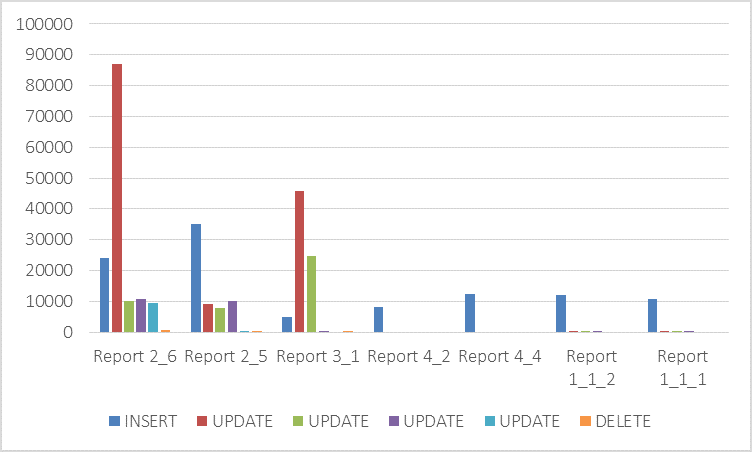
\includegraphics[scale=1]{Pictures/blocks.png}
\caption{Most troublesome statements in the 7 most critical stored procedures}
\label{time graph}
\end{center}
\end{figure}
\noindent As can be seen in Figure \ref{time graph} the \texttt{INSERT} statements take overall the most time to execute, with two large exceptions where the \texttt{UPDATE} statement takes by far much more time to execute.\\ Identifying the tables that would be of interest to alter was done with the help of the stored procedures execution plans. The tables that were chosen were the most resource intensive tables in each execution plan. 
\begin{comment}
\begin{table}[H]
\begin{center}
\begin{tabular}{l|l|l}
Stored Procedures & Troublesome statement & Troublesome Table \\ \hline
Report 2\_6       & \texttt{UPDATE}                & HISTORY\_M        \\ \hline
Report 2\_5       & \texttt{INSERT}                & ITEM              \\ \hline
Report 3\_1       & \texttt{UPDATE}                & ITEM\_L\_E        \\ \hline
Report 4\_2       & \texttt{INSERT}                & HISTORY\_M        \\ \hline
Report 4\_4       & \texttt{INSERT}                & HISTORY\_M        \\ \hline
Report 1\_1\_2    & \texttt{INSERT}                & ITEM              \\ \hline
Report 1\_1\_1    & \texttt{INSERT}                & ITEM              \\
\end{tabular}
\caption{Summary of troublesome tables in the different stored procedures}
\end{center}
\end{table}
\end{comment}
\noindent Three tables where of interest; HISTORY\_M, ITEM and ITEM\_L\_E. These three tables all had a column which could be grouped by dates and had entities with dates stretching back to year 2011. The experimentation started with making copies of the original tables both with and without original indexes and keys and modified stored procedures. The store procedures executions were then time measured and altered by deleting entities associated with a certain year. This measuring and deletion procedure was repeated until entities associated with only one year was left. This procedure was applied to table copies with and without indexes and keys.  
\begin{figure}[H]
\begin{center}$
\begin{array}{c}
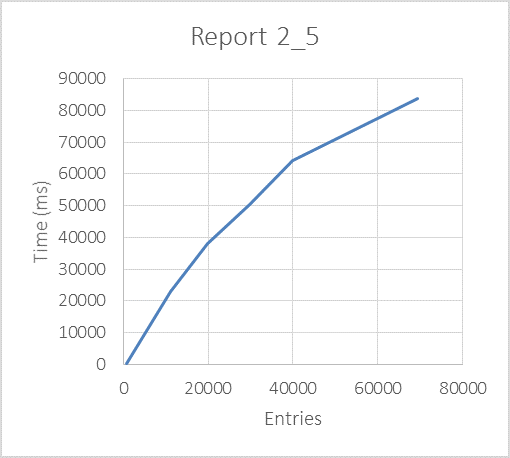
\includegraphics[scale=0.75]{Pictures/Report25.png}  \\ 
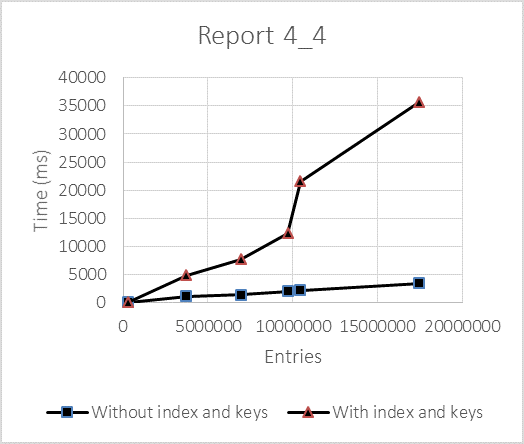
\includegraphics[scale=0.75]{Pictures/Report44.png} \\
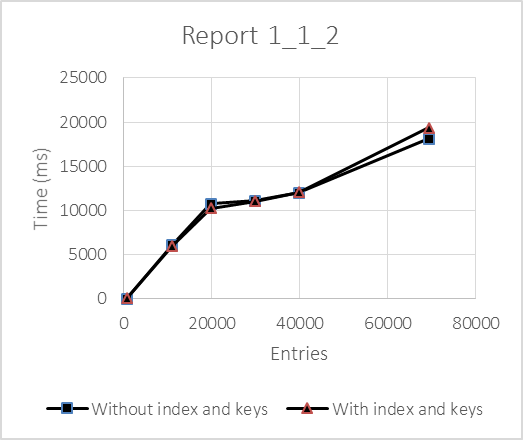
\includegraphics[scale=0.75]{Pictures/Report112.png} 
\end{array}$
\caption{Execution time differences for entity partitioning in troublesome tables}
\label{plots}
\end{center}
\end{figure}\newpage
\noindent The graphs in Figure \ref{plots} are examples of differences this experimentation led to when deleting entities in HISTORY\_M . For almost every procedure the execution time was faster with the original indexes and keys but for report 4\_4 it was the opposite. The stored procedure 4\_4 executed approximately 7 times faster without indexes and keys, indicating that the original indexing and keys are bad performance-wise for report 4\_4. To evaluate future entity growth in the system the experiment also included insertion of entities by copying the original data once more (doubling the number of entities). In most of the cases the execution time increased linearly but for some cases it increased exponentially, as can be seen in Figure \ref{plots}.\\\\
During the experimental entity removals, some anomalies occurred. When deleting rows associated with certain years the execution time seemed to increase compared to prior entity removals. In Figure \ref{anomalie} the stored procedures execution time increased upon deleting entities associated with the years 2011 and 2012 (entities related with year 2013, 2014 and 2015 are still present in the HISTORY\_M table). Additionally deleting entities associated with the year 2013 resulted in a likely manner. This behavior was consistent on both table copies, with and without indexes and keys. 

\begin{figure}[H]
\begin{center}$
\begin{array}{c}
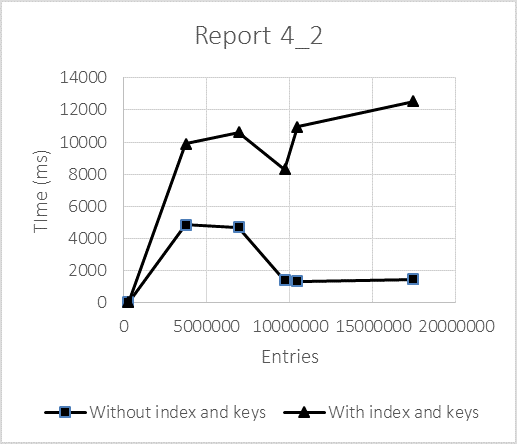
\includegraphics[scale=1.0]{Pictures/anomlie2.png}\\ 
\end{array}$
\caption{Execution time differences for entity partitioning in stored procedure 4\_2}
\label{anomalie}
\end{center}
\vspace{-1cm}
\end{figure}

\noindent During the experimentation it was recognized that the tables ITEM and ITEM\_L\_E could not simply be partitioned since the back-end of the system depended on all of the entries due to sum calculations being made. Therefore further experimentation on those stored procedures who had ITEM and ITEM\_L\_E as problematic tables became also based on alteration of the HISTORY\_M table. Sadly those alterations did not affect the execution time significantly as seen in Figure \ref{alteration}.         

\begin{figure}[H]
\begin{center}$
\begin{array}{c}
\textbf{Alteration on ITEM} \\ 
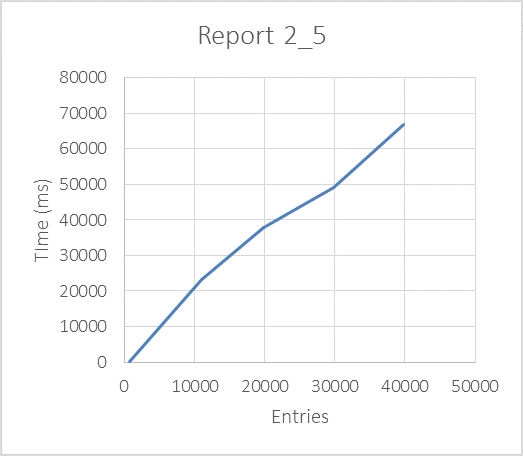
\includegraphics[scale=.95]{Pictures/Report25Index.png}\\
\textbf{Alteration on HISTORY\_M}\\
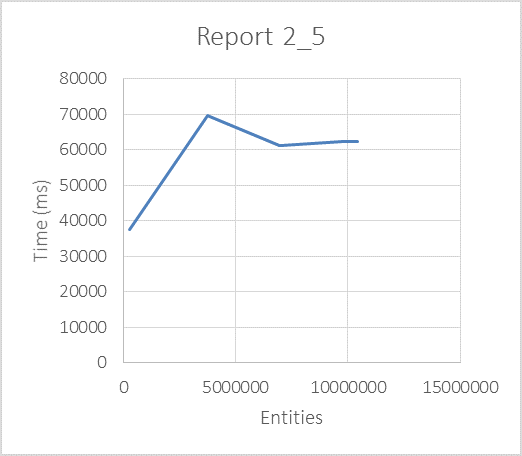
\includegraphics[scale=.95]{Pictures/Report25IndexHistory.png}  
\end{array}$
\caption{Execution time differences for entity partitioning in stored procedure 2\_5}
\label{alteration}
\end{center}
\vspace{-1cm}
\end{figure}

\noindent The above experimentation shows that in some cases table partitioning can reduce the execution time for the BI stored procedures. Unfortunately this cannot be applied on all the heavy resource intensive tables and do not affect significantly in some cases.\\ To complement the experimentation the indexes of the tables were taken under examination.\\ In Figure \ref{indexalteration} three stored procedures are shown with different indexes applied to the table HISTORY\_M, the names of the indexes correspond to the column names in HISTROY\_M. Even here there's evidence of suboptimal indexing. For example in Report 1\_1\_1 and Report 1\_1\_2 the execution time is less when the indexes are removed and maintaining the keys on table HISTORY\_M than having the original indexes and keys on table HISTORY\_M. Even though the new customized indexes didn't result in more efficient execution time, there is room for improvement in index alteration.   

\begin{figure}[H]
\begin{center}$
\begin{array}{c}
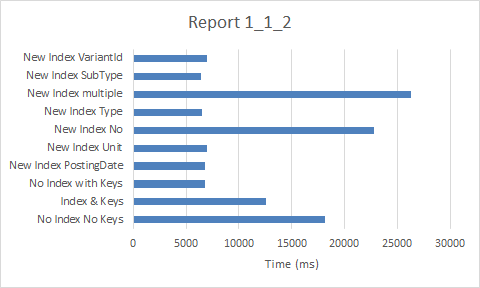
\includegraphics[scale=0.95]{Pictures/Report112IndexAlteration.png} \\
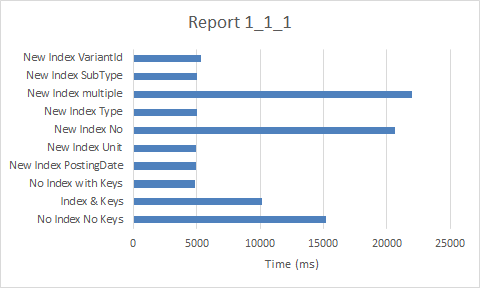
\includegraphics[scale=0.95]{Pictures/Report111IndexAlteration.png} \\
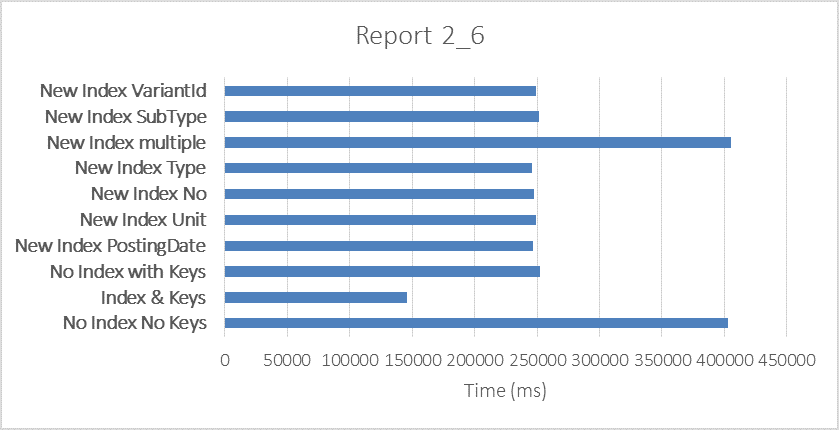
\includegraphics[scale=0.95]{Pictures/Report26IndexAlteration.png} 
\end{array}$
\caption{Execution time differences for index alteration in stored procedures}
\label{indexalteration}
\end{center}
\end{figure}

\subsection{Maintenance plans}
In the current system there is no maintenance done to the database except for the occasional manual adjustments. Since the query execution time is highly affected by the quality of the indexing they should be maintained to make sure that they do not cause bottlenecks. \\\\
Generally a maintenance plan aims to correct or validate three things.
\begin{enumerate}
\item Data and Log file management
\item Index fragmentation
\item Statistics
\end{enumerate}

\noindent Ola Hallengren \cite{Hallengren15} is an award winning database administrator that has released a maintenance script bundle called "SQL Server Maintenance Solution". For these maintenance scripts he has received several community's choice awards and been declared "MVP: Most Valuable Professional" by Microsoft. His scripts are free to use and easy to install. Because of this, the case company's database will be analyzed so that the best implementation of Hallengren's scripts can be used.

\subsubsection{Data and Log File Management}
This topic doesn't necessarily need to be in a regular maintenance plan according to Randal \cite{Randal08}, with the exception of log-file growth. Data and log file management is mostly handled through settings, which should be reviewed so that they follow best practices for performance and security. The following checklist should be considered when looking at these settings.

\begin{enumerate}
\item Data and log files should be separate from each other and isolated from any other systems. (I.e. they should be kept on different drives).
\item Auto-growth is configured correctly.
\item Instant file initialization is configured.
\item Auto-shrink is not enabled and shrink is not part of any maintenance plan.
\end{enumerate}

\noindent Looking at the database system's settings, the data and log files are indeed separate files, but not on different discs. This can cause corruption to the log-file caused by writes by other systems to the disk. This can be a small factor to poorly performing queries, especially the queries that handle large amounts of data. It should be considered to move this file to a separate disk. \\\\
The auto-growth is on and it is set to grow by 10\%. The fact that the auto-grow is set to a percentage can cause an escalation problem with the file size which in turn can cause performance issues. For example, with the auto-grow set to a percentage of file size, the file could first grow with say 10 GB, then 11 GB, then 12 GB and so on even though the rate at which the file grows is constant. Although there is an auto-grow setting, the file sizes should be monitored regularly and proactively grown as part of the maintenance plan, since auto-grow of small amounts can cause file fragmentation and is a time-consuming process which could stall the application workload. The auto-grow setting should still be on though, as a safety net. \\\\
The initial size of the files should be set to an appropriate value based on the file size and the rate at which they grow. These settings has been properly set during the creation of the database system and is not something that is covered in a maintenance plan.\\\\
Shrinking can be used to reduce the size of the data and log files but is a resource-heavy process that causes large amounts of logical read fragmentation in a file. Both auto-shrink and shrinking made by maintenance plans should be avoided. The problems that shrinking tries to solve are better prevented by growing the files at a steady rate. The setting for auto-shrinking is already set to off in the system.

\subsubsection{Index}
Some of the indexes were heavily fragmented. When looking at the tables that use these indexes it was found that those were the tables that are used the most by the system. This indicates that most of the fragmentation caused to those indexes are caused by a high number of transactions, and not necessarily by bad queries. These indexes should therefore be monitored for fragmentation and actions should be taken when necessary to prevent heavy fragmentation. Many maintenance plans however, rebuild or reorganize indexes on a regular basis, without checking if the actual fragmentation is causing problems yet. Since correcting indexes is a high cost procedure, it should only be done when it is necessary. Hallengren's \cite{Hallengren15} scripts monitors the indexes regularly and reorganizes when needed and rebuilds them when it is necessary.

\subsubsection{Statistics}
The default setting in SQL Server is to have auto-update statistics to on. This is also the case in the case company's database. This is good, since statistics need to be accurate and up to date in order for the query planner to do its job properly. There are however advantages to updating statistics manually in a maintenance plan to make sure that they are correct. Updating statistics manually should be done with care. During the index rebuild process the statistics for that index are also updated. If there is a plan to manually update the statistics for that index in the maintenance plan the statistics will be updated twice, which is bad for performance. A manual statistics update is also not as thorough as the update that happens during the rebuild so the statistics might even become worse. If updating statistics should be part of the maintenance plan it should only be done to the indexes that haven't been rebuilt.

\subsubsection{Testing Ola Hallengren's scripts}
Ola Hallengren's maintenance scripts \cite{Hallengren15} were downloaded and set up in the testing environment. The maintenance script require only five simple settings before it could be executed, i.e. which database(s) it should create the script for. When executed the script created four stored procedures that could be used for maintenance and investigation. The main maintenance stored procedure is called schemaname.IndexOptimize. It can be run with a number of settings depending on the requested actions. Some of the key settings is to define what counts as low, medium and high index fragmentation, and what operations that should be performed depending on this level. By default the fragmentation levels are set to Microsoft's recommendation, which are:
\begin{itemize}
\item Low fragmentation < 5\%
\item Medium fragmentation < 30\%
\item High fragmentation > 30\%
\end{itemize}
Notice how there is only a single fragmentation type in these scripts, compared to the two kinds of fragmentation in the theory. The scripts uses the avg\_fragmentation\_in\_percent in sys.dm\_db\_index\_physical\_stats, which is a Microsoft Sql Server feature, to determine the fragmentation.\\\\
The operations that can be performed on an index on each fragmentation level are:
\begin{itemize}
\item Rebuild index online.
\item Rebuild index offline.
\item Reorganize index.
\item Rebuild index online. Rebuild index offline if online rebuilding is not supported on an index. This is the default for a high-fragmented index.
\item Rebuild index online. Reorganize index if online rebuilding is not supported on an index.
\item  Reorganize index. Rebuild index online if reorganizing is not supported on an index. Rebuild index offline if reorganizing and online rebuilding are not supported on an index. 
\item Do not perform index maintenance.
\end{itemize}
Since rebuilding an index can be an expensive operation, reorganizing is preferred on the lower fragmentation levels if the scripts are run often. There are also many more options like setting fill level of the pages and what the least number of pages an index needs to have before it is even considered for maintenance. It's also possible to decide if and when statistics on an index should be updated. Most of these settings have default values based on recommendations from Microsoft.\\\\
When running the script in the test environment a full rebuild of all fragmented indexes was chosen with the rest of the options set to default. After the script had finished, the script used in section \ref{indexfragmentation} was used again to see the results. This showed that all but 14 of the indexes had been rebuild. This is because of the page count lower limit setting, which default value is 1000, and the unaffected indexes were too small to be corrected by the script. To test the result of doing the maintenance the seven slowest performing stored procedures in table \ref{tab:duration} were executed again and the execution times were compared to before the maintenance. Then the maintenance script was run again with a page count lower setting of 100 instead of 1000 to try to catch all indexes. This resulted in all indexes being defragmented. Then the seven slowest performing stored procedures were executed again and the results noted. The results can be seen in Figure \ref{fig:beforeafter}.

\begin{figure}[H]
\begin{center}
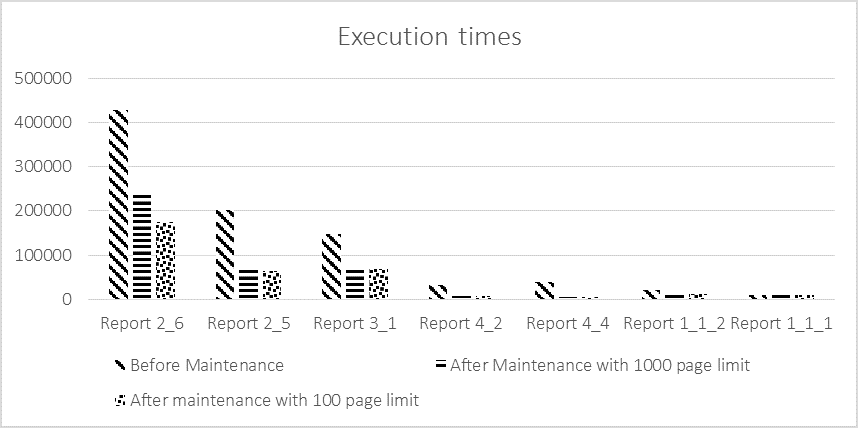
\includegraphics[scale=1]{Pictures/beforeAndAfterMaintenance.png}
\caption{Execution time results from before and after maintenance}
\label{fig:beforeafter}
\end{center}
\end{figure} 

\noindent This drastically shows the effect of having unfragmented indexes and good statistics. Report\_4\_4 for instance, performed 6.5 times faster after the maintenance as seen in Figure \ref{fig:beforeaftertimes}. Report\_1\_1\_1 however showed only a small improvement. The second maintenance run with the lower page limit setting gave a significant performance increase to Report\_2\_5 and Report\_2\_6 but not to the others. This is because of the simple fact that the remaining fragmented indexes were only used in those stored procedures. Performing this maintenance plan doesn't benefit only the BI-reports however, it benefits the whole system. But due to the scope and limitations of this thesis the other areas of the system couldn't be benchmarked.

\begin{figure}[H]
\begin{center}
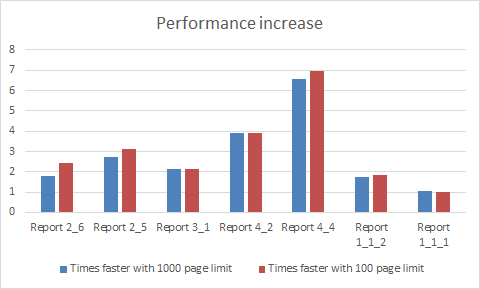
\includegraphics[scale=1]{Pictures/beforeAndAfterMaintenancetimes.png}
\caption{Execution time improvement from the first and second maintenance executions}
\label{fig:beforeaftertimes}
\end{center}
\end{figure}

\subsection{In-memory OLTP}
As described earlier the database system consists of around 250 tables and the particular database that was provided for this thesis is approximately 75GB. Since \bex Online is a cloud bases SaaS solution all of their clients share servers. The database is also increasing in size regarding data content every day. This makes it difficult to put every table in memory since all of the clients databases combined would require hundreds of gigabytes of RAM, which would be very expensive. However, storing only the tables with the most transactions in memory would not take require massive amounts of RAM and could still be notably performance enhancing.
\\\\
By looking at which tables the stored procedures for the business intelligence use in their queries, a pattern could be found. 26 tables are used in all of the stored procedures and another 9 tables are used in more than 80\%. Then there's 46 more tables that are used in less than 20\% of the stored procedures. The 26 tables that are used in all stored procedures contain information that is relatively static, i.e. the information stored in the tables isn't growing at a particularly fast rate. This is preferable when using Hekaton tables since they don't have to be rebuild as often.

\chapter{Proposed Solution}\label{sec:proposedsoluton}
\section{Introduction}
Based on the theory research and the findings made in the analysis a number of solutions to the experienced performance issues can be proposed to the case company.

\section{Table partitioning}
The current database tables in the case company's system are beginning to grow to the point that queries become problematic. As discovered in the analysis in section \ref{Experiments} the performance decreased when entities were eliminated in certain tables. This decrease indicates that archiving and/or table partitioning is something to revise for performance enhancement.
The case company should investigate which of the tables that are most critical for further growth and apply table partitioning on those, considering tables that relate to the BI-report generation. As for example the table HISTORY\_M , which has proven to be a culprit in the system during the analysis.\\
The partitioning should be done horizontally as the system is currently centralized and through \textit{partitioned views} as explained in section \ref{sec:tablepart}. Would the case company however decide to expand the amount of servers and/or decide to make the system distributed a combination of horizontal and vertical partitioning can be applied and should be further researched. The most effective way to partition current tables would be to use the built in table partitioning feature in the Enterprise edition, ergo not alter the current architecture of the system through \textit{partitioned views} but a costly upgrade would be needed.


\section{Maintenance Plan}
Ola Hallengren's \cite{Hallengren15} scripts allow for analysis of the database on a scheduled basis. The scripts then take decisions, based on how they are set up, on what to do with lowly, medium and heavily fragmented indexes separately. For instance, one might want to simply reorganize indexes that have medium fragmentation but rebuild from scratch indexes that are heavily fragmented. Low fragmentation might not be worth the processing resources required to fix them. Since the case company's production environment couldn't be investigated in this thesis, it is hard to give a recommendation on what settings to use in the scripts. But because of the large improvements to the BI-reports performance that was obtained by using the scripts it is highly recommended that these be used. The case company is advised to use these scripts daily to catch performance issues early. Since these scripts require processing resources which could otherwise be used for the actual application, the daily runs should only do light checks and only rebuild the very worst fragmentation. Reorganize, which is a lighter operation is therefore recommended on these. A weekly run with more strict fragmentation and rebuilding options should be performed weekly to make sure that the database is in good condition. Since \bex Online is a system that is used around the clock the rebuilds in the scripts should always be run with the Online option set to On.\\\\
Another finding that the case company should correct is the settings of the data and log file management. The data and log files are recommended to be stored on different disks. They are also recommended to set the auto-growth of the log files to a fixed size instead of the percentage value they use today. This can save space and prevent escalation issues.

\section{In-memory}
Hekaton tables are only available in SQL Server Enterprise edition. The test environment uses SQL Server Standard Edition which meant that experimenting with Hekaton tables wasn't possible. The case company use SQL Server Web Edition which doesn't support Hekaton either. Upgrading to Enterprise Edition is expensive and might not result in any improvements. However, if the case company decides to purchase it, it is highly recommended that they experiment with putting some of their tables with high transaction frequency in memory for overall performance improvements to \bex Online.

\section{Miscellaneous improvements}
As mentioned in the analysis in section \ref{sec:analysis} the execution plans indicated that several issues are present in the current design of queries. One simple reconstruction regarding these queries is to be consistent with the data types. The conversion issues can be a crucial performance diminishment since implicit conversions take place inside the actual table on the specific column scanned specified in the query. Leading to index omittance and consequently more table scans. This can simply be reconstructed in the queries' \texttt{WHERE}-clause by being consistent and investigate that the queried data has the same data type as stated in the query or vise versa. Another solution is to change the data types in the tables.\\
Another possible symptom of implicit data conversion is cardinality estimate issues due to index omittance. This causes the SQL Server optimizer to inadequately estimate the number of rows to fetch and thereupon the need of memory allocation. Low cardinality is a major issue with the case company's current system regarding the BI-reports. The reason for this is versatile and can be because of one or more reasons that are present in the system;  
\begin{center}
\noindent\begin{minipage}[t]{0.5\linewidth}
    \begin{itemize}
    \item Missing or stale statistics
	\item Hidden column correlations
	\item Table variable usage
    \end{itemize}
    \end{minipage}%
    \begin{minipage}[t]{0.4\linewidth}
    \begin{itemize}
    \item Data type issues
	\item Complex predicates
    \end{itemize}
\end{minipage}
\end{center}
\begin{flushright}
Sack \cite{cardinality}
\end{flushright}
\noindent These areas could be the reason for the frequent skew in estimated vs actual output by the SQL Server. To resolve cardinality estimation issues the areas above need to be further investigated and we recommend that in collaboration with a proper maintenance plan, statistics and index updates should be done more often.\\ At the same time the logic and architecture of the SQL in the stored procedure correlated to the BI-reports should be redesigned with more efficient \texttt{INSERT}/\texttt{UPDATE} statements and having data type consistency in mind.
\chapter{Discussion}\label{sec:discussion}

\section{Satisfying the thesis goals}

\subsection{Identifying common database inefficiencies}
The most important areas to consider when identifying database inefficiencies were found mainly in Benjamin Nevarez book  \cite{Nevarez}, and can be seen in section \ref{sec:scope}. The scope of the thesis declared that query tuning, index tuning and "In-Memory OLTP"-solutions were to be investigated. However while performing the research in section \ref{sec:theory}, additional areas of interest were found, e.g. table partitioning and maintenance plans. \\\\
The related work section \ref{sec:related} discusses inefficiencies regarding the actual architecture of relational database system. This was of great interest because it introduced how to get better performance by changing the whole database system instead of just optimizing the current system. The research areas investigated corresponds with what industry experts and researchers recommend and the goal can be considered to be met.

\subsection{BI-process and identifying inefficiencies}
The processes behind the business intelligence reporting in the database system were identified and analyzed. The resulting analysis found several inefficiencies in these processes and the findings were used in the experimentation to find solutions to the issues. This goal was met.

\subsection{"Problem Solving Research"}
The thesis started with finding the underlying issues causing performance problems while generating business intelligence reports. In order to know where to start looking, extensive research was done in order to fully understand the subject and the core areas in its research field. The researched literature was then used to analyze the case company's system to find the relevant bottlenecks and issues. With additional help from the literature, solutions to these problems were found and tested in a test environment. The results from the testing was then used as a foundation for the proposed solution recommended to the case company. This corresponds to the "Problem Solving Research"-methodology.  

\subsection{Analysis of possible solutions}
In section \ref{sec:theory} common issues related to performance in a database system were presented as well as solutions or improvements to these issues. In the analysis section the actual issues with the case company's database system were identified and the solutions that where applicable to these issues were tested where it was possible. These solutions were then analyzed to find if they improved the performance of the business intelligence reports.

\subsection{Solutions}
The solutions to the different performance issues that resulted in a performance increase in the analysis section where presented in the proposed solution section of the thesis. The analysis of these solutions and if they corresponded with the goals of the case company were analyzed and discussed in the proposed solution section in the discussion.

\section{The Proposed Solution}
The proposed solution of this thesis is a set of measures recommended to the case company in order to improve the performance of BI-report generation in their product \bex Online. Due to the limitations (section \ref{sec:limi}) and scope of this thesis (section \ref{sec:scope}) the solutions that were recommended need to be further verified together with \bex Online.\\\\
The recommendations are not a final solution to the case company's problem, however the analysis set up in a test environment is a proof of concept that indicates the proposed solutions would improve performance for BI-report generation. Until the proposed solutions are fully integrated and used in a production environment there's no guarantee that the possible improvements will function as intended.\\\\

\subsection{Omitted theories}
Due to the limitations and the time frame of the thesis some of the theories stated in section \ref{sec:theory} were omitted in the proposed solution. The reasons for this was that the above reasons prevented full research and testing of the areas and consequently other areas became higher prioritized. The areas that were omitted are query tuning, in the form of rewriting the SQL code, and modifying indexing.\\\\During the analysis a few tests were done on index creation and application, these tests did unfortunately not improve the execution in any way. At best they had the same results as the present indexes in the current system. However, through the analysis many areas indicated that indexing was a major inefficiency. When performing table experimentation all the indexes and keys associated with the tables were dropped, which in some cases improved the performance. Implementing different indexes to improve the BI-report generation could improve the execution time, but without any access to the back-end \bex Online there's a great chance index dependencies are unrevealed from the back-end and should not be changed without proper mapping.\\ In collaboration with \bex Online further investigation of the index dependencies is recommended to reveal possibilities of index optimization regarding the tables used by the stored procedures.\\\\
During the research period it became clear that query tuning is one of the most common ways to improve the performance of a query and there is a lot of research done in that area. Most of the research is about the order to perform joins. Throughout the stored procedures joins were frequently used since the data needed were spread out through many tables. The \texttt{JOIN} orderings were therefore very difficult to analyze due to the complexity of the BI-report queries and no findings could be made in this area.\\\\ While analyzing the execution plans another query issue was found. This had to do with SQL Server having to convert values to different data types, i.e. the result table needed the value as one data type but it was retrieved as another. This issue couldn't be solved since that would imply architectural alterations on the current tables in the system. The queries mentioned above also had extensive \texttt{WHERE}-clauses where the data that was required was filtered with many prerequisite variables. These \texttt{WHERE}-clauses together with the \texttt{JOIN} ordering should be revised and further investigated by the case company.\\\\ As mentioned in section \ref{sec:sp} the structure of the stored procedures were somewhat similar with \texttt{INSERT}-, several \texttt{UPDATE}s- and in some cases \texttt{DELETE}-statements. With a swift experimentation that consisted of doing the \texttt{INSERT}-statement and \texttt{UPDATE}-statement simultaneously, i.e. merge or include the \texttt{UPDATE}-statement in the \texttt{INSERT}-statement, showed through the estimated execution plan that the affected tables weren't iterated as many times. No further experimentation was conducted on query destructing considering it's highly time consuming and could in itself support a whole other master thesis subject. Therefore the logic and structure of the SQL in the stored procedures should be taken into consideration if the case company decides to improve the performance through query tuning.        

\section{Table partitioning}
The necessity of table partitioning was examined through a simulation of actual table partitioning, which as of the SQL Server 2005 is a built in function. However, this built in function only applies to the Enterprise edition of Microsoft SQL Server. This, according to King \cite{partitionwoEnterprise}, is due to that Microsoft and others argue that if a company has the need of doing table partitioning they have a large amount of data. Which in turn equals a large company, which in turn equals financial wealth and that upgrading to an Enterprise edition is therefore not a great obstacle. \\ In the same article as mentioned above, King states that table partitioning is possible for every current SQL Server edition by using partitioned views.\\ This method offers nearly all the benefits from "true partitioning". Sadly it includes schema architecture alteration, which with this thesis's limitations doesn't coincide. Consequently a simulation where entities were deleted from tables, instead of using the built in partitioning function or partitioned views, was done.\\
The anomalies stated in section \ref{Experiments} could be due to omitted table index and statistics rebuilds in between entity deletion. Applying rebuilds of table index and statistics between the deletions did unfortunately not result in any change. \\\\
Should the case company want to apply table partitioning to their system, a self made solution as done in this thesis is not recommended. We would recommend to choose the built in function in the Enterprise edition, ergo upgrading the server edition. If that option is too costly for the case company, further research about the compensated solution partitioned views should be done to evaluate if it covers the desired improvements. 

\section{Maintenance plan}
The maintenance plan-part of the thesis started as a result of the analysis of the index fragmentation. During the theory research a lot of references to good maintenance planning came up, and especially to Ola Hallengren's scripts \cite{Hallengren15}. These scripts were easy to implement and resulted in three easy to use stored procedures for maintenance. During the testing of the scripts the setting to defragment all indexes was chosen. This is unnecessarily demanding processing wise to do but was performed in order to achieve the best possible performance during the benchmarking. As declared in the proposed solution the case company should consider only performing index rebuilds when it's very necessary, and do maintenance procedures that only require light processing more often. During research, many different disciplines of setting up a maintenance plan were found. There were no specific ways that were better than others. The different ways had more to do with that DBAs personal views and the specific database system. While the company should consider the solution proposed in the thesis, the company should also experiment and see what the best result they can achieve is while keeping the processing overhead low. 

\section{In-memory}
During the research period of the thesis In-Memory solutions were discussed as very promising performance enhancing solutions. The case company also specifically requested solutions that included putting part of the database system in RAM. Microsoft SQL Server has it's built in Hekaton module but it is only available in the Enterprise edition which is very expensive to license. This made it unfeasible to test during this thesis. The sheer size of all \bex Online's customers databases together makes the required amount of RAM very large which causes further problems. The case company is however recommended to experiment with In-Memory database solutions due to results in other peoples work. A technology called Speedment \cite{speedment} was also researched but didn't make it into the thesis since it didn't yet have support for Microsoft SQL Server. Tests performed with that technology has given very promising results and the company behind it claims that they can make all searches for data with $\mathcal{O}(1)$ time complexity. When Speedment releases support for SQL server the case company should investigate to see if it is applicable to \bex Online.

\section{Future improvement recommendations}
As Perfect IT BeX AB has had an increase in clients and plans to expand even more, the current system would need to do so as well. Currently only one physical server handles all the data and transactions done by \bex clients. Expanding the amount of servers could induce the possibility of distributing the performance load and the data to the different servers. A first step would preferably be to put \bex Online on one server and the database system on another. This would make it easier to perform load balancing and later investing in more servers depending on which module that needs it. Also, it enables the case company to switch to a distributed database system as the product scales.\\\\
There is a concept called "Database Partitioning" that has shown promising performance enhancing results and that can be of interest to the case company. Database partitioning can be either logical or physical. A multi-partition environment improves the performance and the scalability of very large databases, and allows very complex queries to execute much faster.\\\\
Another recommendation to the company is to consider investing in a SQL Server Enterprise edition. This would allow them to investigate the built-in In-memory solution, table partitioning and it would allow them to use more RAM since the other versions have a limit of 64 GB. This investment is expensive however and the benefits has to be weighed against the cost.

\chapter{Conclusions}\label{sec:conclusions}
\section{Research}
Due to the limitations and directions from the case company, \bex Online's database system was chosen as the area to investigate. The thesis started with doing a lot of research on database optimization. The subject is widely researched and there is constant work in the field, which allowed the authors to choose between many different directions when solving the problem. The areas that were chosen to further investigate were:
\begin{itemize}
\item Query tuning
\item Execution statistics
\item Indexing
\item Index fragmentation
\item Maintenance planning
\item Table partitioning
\item In-Memory OLTP
\end{itemize}

\subsection{Analysis and testing}
The analysis and testing was performed in a copy of the production database system in an environment that was different from the production environment. This means that there is a risk that constant updates to the production system could cause integration issues with the proposed solution.
Since the analysis and testing was made in a test environment with poorer system specifications and thus the benchmark times are larger than they would be in the production system. The performance improvements that were discovered however should have the corresponding effect in production.\\\\ The analysis found that the best improvements to the database system could be made in table partitioning and setting up a proper maintenance plan. This improved the performance of some queries by up to $6\frac{1}{2}$ times. The analysis also found that performance most likely can be further improved by utilizing In-Memory database solutions. Unfortunately the SQL Server version used in the testing environment didn't include Microsoft's own In-Memory solution, Hekaton. The case company is however recommended to experiment with this if the decide to upgrade to the Enterprise edition. 

\addcontentsline{toc}{chapter}{Bibliography}
\bibliographystyle{ieeetr}

\bibliography{MyMSc}

\begin{appendices}

\chapter{Code} \label{appCode}
\begin{lstlisting}[caption={Algorithm to find fragmented tables and the fragmentation values},label=See DB-Fragmentation]
SELECT object_name(dt.object_id) Tablename,si.name
IndexName,dt.avg_fragmentation_in_percent AS
ExternalFragmentation,dt.avg_page_space_used_in_percent AS
InternalFragmentation
FROM
(
    SELECT object_id,index_id,avg_fragmentation_in_percent,avg_page_space_used_in_percent
    FROM sys.dm_db_index_physical_stats (db_id('AdventureWorks'),null,null,null,'DETAILED'
)
WHERE index_id <> 0) AS dt INNER JOIN sys.indexes si ON si.object_id=dt.object_id
AND si.index_id=dt.index_id AND dt.avg_fragmentation_in_percent>10
AND dt.avg_page_space_used_in_percent<75 ORDER BY avg_fragmentation_in_percent DESC
\end{lstlisting}


\begin{lstlisting}[caption={Example of broken-down query, instead of OR operator in WHERE clause on two different tables},label=firstbreak-down]
SELECT SalesOrderID FROM Sales.SalesOrderDetail
WHERE ProductID=897
SELECT SalesOrderID FROM Sales.SalesOrderHeader
WHERE CustomerID=11020
\end{lstlisting}
\newpage

\begin{lstlisting}[caption={UNION instead of OR},label=second-down]
SELECT SalesOrderID FROM Sales.SalesOrderHeader soh
	JOIN Sales.SalesOrderDetail sod
	ON soh.SalesOrderID=sod.SalesOrderID
WHERE sod.ProductID=897
UNION
SELECT SalesOrderID FROM Sales.SalesOrderHeader soh
	JOIN Sales.SalesOrderDetail sod
	ON soh.SalesOrderID=sod.SalesOrderID
WHERE soh.CustomerID=11020
\end{lstlisting} 


\begin{lstlisting}[caption={SQL batch to execute stored procedure report\_2\_5},label=spexec]
USE [bex_bob]
GO
set statistics IO on
set statistics time on
DECLARE	@return_value int

EXEC	@return_value = [dbo].[report_2_5]
		@headerId = 75642,
		@Unit = 10,
		@PurchaseDate1 = '',
		@PurchaseDate2 = '',
		@SalesDate1 = N'2014-01-01',
		@SalesDate2 = N'2015-01-01',
		@StockDate = N'2015-01-01',
		@includeInternal = 1,
		@LocationCode = '',
		@SupplierNo = '',
		@ItemGroupCode = '',
		@ItemCategoryCode = '',
		@ProductGroupCode = '',
		@ProgramCode = '',
		@Collection = '',
		@Gender = -1

SELECT	'Return Value' = @return_value

GO
set statistics IO off
set statistics time off
SELECT * FROM EXT_REPORT_RESULT_2_5
\end{lstlisting}

\newpage
\begin{lstlisting}[caption={SQL batch to create a partitioned table out of an already existing table},label=partitionex]
CREATE PARTITION FUNCTION partitionFunction (datetime)
AS RANGE RIGHT FOR VALUES ('20120101','20130101','20140101','20150101')
GO
CREATE PARTITION SCHEME partitionScheme 
AS PARTITION partitionfunction ALL TO ([PRIMARY]) 
GO
ALTER TABLE dbo.HISTORY_M DROP CONSTRAINT PK_HISTORY_M
GO
ALTER TABLE dbo.HISTORY_M ADD CONSTRAINT
 PK_HISTORY_M PRIMARY KEY NONCLUSTERED  (pkcol)
   WITH (STATISTICS_NORECOMPUTE = OFF, IGNORE_DUP_KEY = OFF, 
         ALLOW_ROW_LOCKS = ON, ALLOW_PAGE_LOCKS = ON) ON [PRIMARY]
GO
CREATE CLUSTERED INDEX IX_HISTORY_M_partitioncol ON
 dbo.HISTORY_M(partitioncol)
  WITH (STATISTICS_NORECOMPUTE = OFF, IGNORE_DUP_KEY = OFF, 
        ALLOW_ROW_LOCKS = ON, ALLOW_PAGE_LOCKS = ON) 
  ON partitionScheme(partitioncol)

\end{lstlisting}



\chapter{Environments}
\section{General Environment}\label{sec:Genviron}
\begin{table}[H]
\begin{center}
\caption*{\textbf{Server}}
\begin{tabular}{l l}
OS: & Windows Server 2012 Standard 64-bit\\
CPU: & Intel(R) Xeon(R) CPU E5-2440 @ 2.40 GHz 64-bit based\\
RAM: & 64 GB \\
HD: & 500 GB Disk drive
\end{tabular}
\end{center}
\end{table}

\section{Analysis \& Test Environment}\label{Aenviron}
\begin{table}[H]
\begin{center}
\caption*{\textbf{Local System}}
\begin{tabular}{l l}
OS: & Windows 8.1 64-bit\\
CPU: & Intel Quad-Core I7 4GHz\\
RAM: & 16Gb, 1566Hz\\
HD: & 3 TB 7200 RPM Disk drive \\
Tools/Programs: & SQL Server Management Studio, SQL Sentry Plan Explorer\\
\end{tabular}
\end{center}
\end{table}

\chapter{Large Illustrations and Tables}\label{sec:appTabIll}
\begin{table}[H]
\centering
\scalebox{0.8}{
\begin{tabular}{  l | l | l | l | l | l | l | l  H   H   H   H   H   H   H   H   H   H   H   H   H   H   H   H   H   H   H   H   H   H   H  l | l  }
\LARGE{Table}&\multicolumn{29}{c}{\LARGE{Stored procedure for BI-report}}& \\\hline

	 & 1\_1\_1 & 1\_1\_2 & 1\_1\_3 & 1\_1\_4 & 1\_1\_5 & 1\_1\_6 &1\_1\_7 & 1\_1\_8 & 1\_1\_9 & 1\_2\_2 & 1\_3\_2 & 1\_5\_1 & 1\_5\_2 & 1\_5\_7 & 1\_6\_1 & 2\_1\_1 & 2\_1\_2 & 2\_5 & 2\_6 & 3\_1 & 3\_2 & 3\_3 & 3\_4 & 3\_5 & 3\_6 & 3\_7 & 4\_2 & 4\_3 & 4\_4 & 4\_5 & \dots & TOTAL \\ \hline
	 BO\_U & X & X & X & X & X & X & X & X & X & X & X & X & X & X & X & X & X & X & X & X & X & X & X & X & X & X & X & X & X & X & \dots & 30 \\ \hline
	 COLLECTION & X & X & X & X & X & X & X & X & X & X & X & X & X & X & X & X & X & X & X & X & X & X & X & X & X & X & X & X & X & X & \dots & 30 \\ \hline
	 COLOUR\_G & X & X & X & X & X & X & X & X & X & X & X & X & X & X & X & X & X & X & X & X & X & X & X & X & X & X & X & X & X & X  & \dots & 30 \\ \hline
	 COUNTRY & X & X & X & X & X & X & X & X & X & X & X & X & X & X & X & X & X & X & X & X & X & X & X & X & X & X & X & X & X & X  & \dots & 30 \\ \hline
	 CUSTOMER & X & X & X & X & X & X & X & X & X & X & X & X & X & X & X & X & X & X & X & X & X & X & X & X & X & X & X & X & X & X  & \dots & 30 \\ \hline
	 CUSTOMER\_G & X & X & X & X & X & X & X & X & X & X & X & X & X & X & X & X & X & X & X & X & X & X & X & X & X & X & X & X & X & X  & \dots & 30 \\ \hline
	 CUSTOMER\_I\_D & X & X & X & X & X & X & X & X & X & X & X & X & X & X & X & X & X & X & X & X & X & X & X & X & X & X & X & X & X & X  & \dots & 30 \\ \hline
	 CUSTOMER\_P\_G & X & X & X & X & X & X & X & X & X & X & X & X & X & X & X & X & X & X & X & X & X & X & X & X & X & X & X & X & X & X  & \dots & 30 \\ \hline
	 DIMENSION2 & X & X & X & X & X & X & X & X & X & X & X & X & X & X & X & X & X & X & X & X & X & X & X & X & X & X & X & X & X & X  & \dots & 30 \\ \hline
	 ITEM & X & X & X & X & X & X & X & X & X & X & X & X & X & X & X & X & X & X & X & X & X & X & X & X & X & X & X & X & X & X  & \dots & 30 \\ \hline
	 ITEM\_CA & X & X & X & X & X & X & X & X & X & X & X & X & X & X & X & X & X & X & X & X & X & X & X & X & X & X & X & X & X & X  & \dots & 30 \\ \hline
	 ITEM\_CO & X & X & X & X & X & X & X & X & X & X & X & X & X & X & X & X & X & X & X & X & X & X & X & X & X & X & X & X & X & X  & \dots & 30 \\ \hline
	 ITEM\_F & X & X & X & X & X & X & X & X & X & X & X & X & X & X & X & X & X & X & X & X & X & X & X & X & X & X & X & X & X & X  & \dots & 30 \\ \hline
	 ITEM\_GE & X & X & X & X & X & X & X & X & X & X & X & X & X & X & X & X & X & X & X & X & X & X & X & X & X & X & X & X & X & X  & \dots & 30 \\ \hline
	 ITEM\_GR & X & X & X & X & X & X & X & X & X & X & X & X & X & X & X & X & X & X & X & X & X & X & X & X & X & X & X & X & X & X  & \dots & 30 \\ \hline
	 ITEM\_I & X & X & X & X & X & X & X & X & X & X & X & X & X & X & X & X & X & X & X & X & X & X & X & X & X & X & X & X & X & X  & \dots & 30 \\ \hline
	 ITEM\_V & X & X & X & X & X & X & X & X & X & X & X & X & X & X & X & X & X & X & X & X & X & X & X & X & X & X & X & X & X & X  & \dots & 30 \\ \hline
	 LENGTH\_G & X & X & X & X & X & X & X & X & X & X & X & X & X & X & X & X & X & X & X & X & X & X & X & X & X & X & X & X & X & X  & \dots & 30 \\ \hline
	 LOCATIONS & X & X & X & X & X & X & X & X & X & X & X & X & X & X & X & X & X & X & X & X & X & X & X & X & X & X & X & X & X & X  & \dots & 30 \\ \hline
	 PRODUCT\_G & X & X & X & X & X & X & X & X & X & X & X & X & X & X & X & X & X & X & X & X & X & X & X & X & X & X & X & X & X & X  & \dots & 30 \\ \hline
	 PROGRAM & X & X & X & X & X & X & X & X & X & X & X & X & X & X & X & X & X & X & X & X & X & X & X & X & X & X & X & X & X & X  & \dots & 30 \\ \hline
	 REPORT\_H & X & X & X & X & X & X & X & X & X & X & X & X & X & X & X & X & X & X & X & X & X & X & X & X & X & X & X & X & X & X  & \dots & 30 \\ \hline
	 SALESPERSON & X & X & X & X & X & X & X & X & X & X & X & X & X & X & X & X & X & X & X & X & X & X & X & X & X & X & X & X & X & X  & \dots & 30 \\ \hline
	 SHOP & X & X & X & X & X & X & X & X & X & X & X & X & X & X & X & X & X & X & X & X & X & X & X & X & X & X & X & X & X & X  & \dots & 30 \\ \hline
	 SIZE\_G & X & X & X & X & X & X & X & X & X & X & X & X & X & X & X & X & X & X & X & X & X & X & X & X & X & X & X & X & X & X  & \dots & 30 \\ \hline
	 SUPPLIER & X & X & X & X & X & X & X & X & X & X & X & X & X & X & X & X & X & X & X & X & X & X & X & X & X & X & X & X & X & X  & \dots & 30 \\ \hline
\end{tabular}}
\caption{tables used among all stored procedures for BI-reports}
\label{tab:tabinall}
\end{table}


\newgeometry{left=0.2cm, right=0.5cm, bottom=3cm}
\begin{table}[H]
\centering
\resizebox{\textwidth}{!}{
\begin{tabular}{  l | c | c | c | c | c | c | c | c | c | c | c | c | c | c | c | c | c | c | c | c | c | c | c | c | c | c | c | c | c | c | c  }
\LARGE{Table}&\multicolumn{29}{c}{\LARGE{Stored procedure for BI-report}}& \\\hline
	 & 1\_1\_1 & 1\_1\_2 & 1\_1\_3 & 1\_1\_4 & 1\_1\_5 & 1\_1\_6 & 1\_1\_7 & 1\_1\_8 & 1\_1\_9 & 1\_2\_2 & 1\_3\_2 & 1\_5\_1 & 1\_5\_2 & 1\_5\_7 & 1\_6\_1 & 2\_1\_1 & 2\_1\_2 & 2\_5 & 2\_6 & 3\_1 & 3\_2 & 3\_3 & 3\_4 & 3\_5 & 3\_6 & 3\_7 & 4\_2 & 4\_3 & 4\_4 & 4\_5 & TOTAL \\ \hline
	 ACCOUNT & X & X & X & X & X & X & X & X & X & X & X &  &  &  & X & X & X & X & X &  & X & X & X & X & X &  & X & X & X & X & 25 \\ \hline
	 BO\_U & X & X & X & X & X & X & X & X & X & X & X & X & X & X & X & X & X & X & X & X & X & X & X & X & X & X & X & X & X & X & 30 \\ \hline
	 COLLECTION & X & X & X & X & X & X & X & X & X & X & X & X & X & X & X & X & X & X & X & X & X & X & X & X & X & X & X & X & X & X & 30 \\ \hline
	 COLOUR\_G & X & X & X & X & X & X & X & X & X & X & X & X & X & X & X & X & X & X & X & X & X & X & X & X & X & X & X & X & X & X & 30 \\ \hline
	 COMPANY\_I &  &  &  &  &  &  &  &  &  &  &  & X & X & X &  &  &  & X & X & X &  &  &  &  &  & X &  &  &  &  & 7 \\ \hline
	 COUNTRY & X & X & X & X & X & X & X & X & X & X & X & X & X & X & X & X & X & X & X & X & X & X & X & X & X & X & X & X & X & X & 30 \\ \hline
	 CUSTOMER & X & X & X & X & X & X & X & X & X & X & X & X & X & X & X & X & X & X & X & X & X & X & X & X & X & X & X & X & X & X & 30 \\ \hline
	 CUSTOMER\_G & X & X & X & X & X & X & X & X & X & X & X & X & X & X & X & X & X & X & X & X & X & X & X & X & X & X & X & X & X & X & 30 \\ \hline
	 CUSTOMER\_I\_D & X & X & X & X & X & X & X & X & X & X & X & X & X & X & X & X & X & X & X & X & X & X & X & X & X & X & X & X & X & X & 30 \\ \hline
	 CUSTOMER\_L\_E & X & X & X & X & X & X & X & X & X & X & X &  &  &  & X & X & X & X & X &  & X & X & X & X & X &  & X & X & X & X & 25 \\ \hline
	 CUSTOMER\_P\_G & X & X & X & X & X & X & X & X & X & X & X & X & X & X & X & X & X & X & X & X & X & X & X & X & X & X & X & X & X & X & 30 \\ \hline
	 CUSTOMER\_P\_G &  &  &  &  &  &  &  &  &  &  &  &  &  &  &  &  &  &  &  &  & X &  &  &  &  &  &  &  &  &  & 1 \\ \hline
	 DELIVERYCHANGE\_R &  &  &  &  &  &  &  &  &  &  &  & X & X & X &  &  &  & X & X & X &  &  &  &  &  & X &  &  &  &  & 7 \\ \hline
	 DIMENSION1 & X & X & X & X & X & X & X & X & X & X & X &  &  &  & X & X & X & X & X &  & X & X & X & X & X &  & X & X & X & X & 25 \\ \hline
	 DIMENSION2 & X & X & X & X & X & X & X & X & X & X & X & X & X & X & X & X & X & X & X & X & X & X & X & X & X & X & X & X & X & X & 30 \\ \hline
	 DISC\_C &  &  &  &  &  &  &  &  &  &  & X &  &  &  &  &  &  &  &  &  &  &  &  &  &  &  &  &  &  &  & 1 \\ \hline
	 HISTORY\_M & X & X & X & X & X & X & X & X & X & X & X &  &  &  & X & X & X & X & X &  & X & X & X & X & X &  & X & X & X & X & 25 \\ \hline
	 ITEM & X & X & X & X & X & X & X & X & X & X & X & X & X & X & X & X & X & X & X & X & X & X & X & X & X & X & X & X & X & X & 30 \\ \hline
	 ITEM\_CA & X & X & X & X & X & X & X & X & X & X & X & X & X & X & X & X & X & X & X & X & X & X & X & X & X & X & X & X & X & X & 30 \\ \hline
	 ITEM\_CO & X & X & X & X & X & X & X & X & X & X & X & X & X & X & X & X & X & X & X & X & X & X & X & X & X & X & X & X & X & X & 30 \\ \hline
	 ITEM\_F & X & X & X & X & X & X & X & X & X & X & X & X & X & X & X & X & X & X & X & X & X & X & X & X & X & X & X & X & X & X & 30 \\ \hline
	 ITEM\_GE & X & X & X & X & X & X & X & X & X & X & X & X & X & X & X & X & X & X & X & X & X & X & X & X & X & X & X & X & X & X & 30 \\ \hline
	 ITEM\_GR & X & X & X & X & X & X & X & X & X & X & X & X & X & X & X & X & X & X & X & X & X & X & X & X & X & X & X & X & X & X & 30 \\ \hline
	 ITEM\_I & X & X & X & X & X & X & X & X & X & X & X & X & X & X & X & X & X & X & X & X & X & X & X & X & X & X & X & X & X & X & 30 \\ \hline
	 ITEM\_L\_E & X & X & X & X & X & X & X & X & X & X & X &  &  &  & X & X & X & X & X & X & X & X & X & X & X & X & X & X & X & X & 27 \\ \hline
	 ITEM\_V & X & X & X & X & X & X & X & X & X & X & X & X & X & X & X & X & X & X & X & X & X & X & X & X & X & X & X & X & X & X & 30 \\ \hline
	 LENGTH\_G & X & X & X & X & X & X & X & X & X & X & X & X & X & X & X & X & X & X & X & X & X & X & X & X & X & X & X & X & X & X & 30 \\ \hline
	 LOCATIONS & X & X & X & X & X & X & X & X & X & X & X & X & X & X & X & X & X & X & X & X & X & X & X & X & X & X & X & X & X & X & 30 \\ \hline
	 ORDER\_T &  &  &  &  &  &  &  &  &  &  &  & X & X & X &  &  &  & X & X & X &  &  &  &  &  & X &  &  &  &  & 7 \\ \hline
	 POSTING\_G\_I & X & X & X & X & X & X & X & X & X & X & X &  &  &  & X & X & X & X & X &  & X & X & X & X & X &  & X & X & X & X & 25 \\ \hline
	 POSTING\_S &  &  &  &  &  &  &  &  &  &  &  &  &  &  &  &  &  &  &  &  & X &  &  &  &  &  &  &  &  &  & 1 \\ \hline
	 PRODUCT\_G & X & X & X & X & X & X & X & X & X & X & X & X & X & X & X & X & X & X & X & X & X & X & X & X & X & X & X & X & X & X & 30 \\ \hline
	 PROGRAM & X & X & X & X & X & X & X & X & X & X & X & X & X & X & X & X & X & X & X & X & X & X & X & X & X & X & X & X & X & X & 30 \\ \hline
	 PURCHASE\_H &  &  &  &  &  &  &  &  &  &  &  & X & X & X &  &  &  & X & X & X &  &  &  &  &  & X &  &  &  &  & 7 \\ \hline
	 PURCHASE\_L &  &  &  &  &  &  &  &  &  &  &  & X & X & X &  &  &  & X & X & X &  &  &  &  &  & X &  &  &  &  & 7 \\ \hline
	 REATAIL\_C &  &  &  &  &  &  &  &  &  &  &  & X & X & X &  &  &  & X & X & X &  &  &  &  &  & X &  &  &  &  & 7 \\ \hline
	 REPORT\_H & X & X & X & X & X & X & X & X & X & X & X & X & X & X & X & X & X & X & X & X & X & X & X & X & X & X & X & X & X & X & 30 \\ \hline
	 REPORT\_RESULT\_1\_1\_1 & X &  &  &  &  &  &  &  &  &  &  &  &  &  &  &  &  &  &  &  &  &  &  &  &  &  &  &  &  &  & 1 \\ \hline
	 REPORT\_RESULT\_1\_1\_2 &  & X &  &  &  &  &  &  &  &  &  &  &  &  &  &  &  &  &  &  &  &  &  &  &  &  &  &  &  &  & 1 \\ \hline
	 REPORT\_RESULT\_1\_1\_3 &  &  & X &  &  &  &  &  &  &  &  &  &  &  &  &  &  &  &  &  &  &  &  &  &  &  &  &  &  &  & 1 \\ \hline
	 REPORT\_RESULT\_1\_1\_4 &  &  &  & X &  &  &  &  &  &  &  &  &  &  &  &  &  &  &  &  &  &  &  &  &  &  &  &  &  &  & 1 \\ \hline
	 REPORT\_RESULT\_1\_1\_5 &  &  &  &  & X &  &  &  &  &  &  &  &  &  &  &  &  &  &  &  &  &  &  &  &  &  &  &  &  &  & 1 \\ \hline
	 REPORT\_RESULT\_1\_1\_6 &  &  &  &  &  & X &  &  &  &  &  &  &  &  &  &  &  &  &  &  &  &  &  &  &  &  &  &  &  &  & 1 \\ \hline
	 REPORT\_RESULT\_1\_1\_7 &  &  &  &  &  &  & X &  &  &  &  &  &  &  &  &  &  &  &  &  &  &  &  &  &  &  &  &  &  &  & 1 \\ \hline
	 REPORT\_RESULT\_1\_1\_8 &  &  &  &  &  &  &  & X &  &  &  &  &  &  &  &  &  &  &  &  &  &  &  &  &  &  &  &  &  &  & 1 \\ \hline
	 REPORT\_RESULT\_1\_1\_9 &  &  &  &  &  &  &  &  & X &  &  &  &  &  &  &  &  &  &  &  &  &  &  &  &  &  &  &  &  &  & 1 \\ \hline
	 REPORT\_RESULT\_1\_2\_2 &  &  &  &  &  &  &  &  &  & X &  &  &  &  &  &  &  &  &  &  &  &  &  &  &  &  &  &  &  &  & 1 \\ \hline
	 REPORT\_RESULT\_1\_3\_2 &  &  &  &  &  &  &  &  &  &  & X &  &  &  &  &  &  &  &  &  &  &  &  &  &  &  &  &  &  &  & 1 \\ \hline
	 REPORT\_RESULT\_1\_5\_1 &  &  &  &  &  &  &  &  &  &  &  & X &  &  &  &  &  &  &  &  &  &  &  &  &  &  &  &  &  &  & 1 \\ \hline
	 REPORT\_RESULT\_1\_5\_2 &  &  &  &  &  &  &  &  &  &  &  &  & X &  &  &  &  &  &  &  &  &  &  &  &  &  &  &  &  &  & 1 \\ \hline
	 REPORT\_RESULT\_1\_5\_7 &  &  &  &  &  &  &  &  &  &  &  &  &  & X &  &  &  &  &  &  &  &  &  &  &  &  &  &  &  &  & 1 \\ \hline
	 REPORT\_RESULT\_1\_6\_1 &  &  &  &  &  &  &  &  &  &  &  &  &  &  & X &  &  &  &  &  &  &  &  &  &  &  &  &  &  &  & 1 \\ \hline
	 REPORT\_RESULT\_2\_1\_1 &  &  &  &  &  &  &  &  &  &  &  &  &  &  &  & X &  &  &  &  &  &  &  &  &  &  &  &  &  &  & 1 \\ \hline
	 REPORT\_RESULT\_2\_1\_2 &  &  &  &  &  &  &  &  &  &  &  &  &  &  &  &  & X &  &  &  &  &  &  &  &  &  &  &  &  &  & 1 \\ \hline
	 REPORT\_RESULT\_2\_5 &  &  &  &  &  &  &  &  &  &  &  &  &  &  &  &  &  & X &  &  &  &  &  &  &  &  &  &  &  &  & 1 \\ \hline
	 REPORT\_RESULT\_2\_6 &  &  &  &  &  &  &  &  &  &  &  &  &  &  &  &  &  &  & X &  &  &  &  &  &  &  &  &  &  &  & 1 \\ \hline
	 REPORT\_RESULT\_3\_1 &  &  &  &  &  &  &  &  &  &  &  &  &  &  &  &  &  &  &  & X &  &  &  &  &  &  &  &  &  &  & 1 \\ \hline
	 REPORT\_RESULT\_3\_2 &  &  &  &  &  &  &  &  &  &  &  &  &  &  &  &  &  &  &  &  & X &  &  &  &  &  &  &  &  &  & 1 \\ \hline
	 REPORT\_RESULT\_3\_3 &  &  &  &  &  &  &  &  &  &  &  &  &  &  &  &  &  &  &  &  &  & X &  &  &  &  &  &  &  &  & 1 \\ \hline
	 REPORT\_RESULT\_3\_4 &  &  &  &  &  &  &  &  &  &  &  &  &  &  &  &  &  &  &  &  &  &  & X &  &  &  &  &  &  &  & 1 \\ \hline
	 REPORT\_RESULT\_3\_5 &  &  &  &  &  &  &  &  &  &  &  &  &  &  &  &  &  &  &  &  &  &  &  & X &  &  &  &  &  &  & 1 \\ \hline
	 REPORT\_RESULT\_3\_6 &  &  &  &  &  &  &  &  &  &  &  &  &  &  &  &  &  &  &  &  &  &  &  &  & X &  &  &  &  &  & 1 \\ \hline
	 REPORT\_RESULT\_3\_7 &  &  &  &  &  &  &  &  &  &  &  &  &  &  &  &  &  &  &  &  &  &  &  &  &  & X &  &  &  &  & 1 \\ \hline
	 REPORT\_RESULT\_3\_7\_SUB1 &  &  &  &  &  &  &  &  &  &  &  &  &  &  &  &  &  &  &  &  &  &  &  &  &  & X &  &  &  &  & 1 \\ \hline
	 REPORT\_RESULT\_4\_2 &  &  &  &  &  &  &  &  &  &  &  &  &  &  &  &  &  &  &  &  &  &  &  &  &  &  & X &  &  &  & 1 \\ \hline
	 REPORT\_RESULT\_4\_3 &  &  &  &  &  &  &  &  &  &  &  &  &  &  &  &  &  &  &  &  &  &  &  &  &  &  &  & X &  &  & 1 \\ \hline
	 REPORT\_RESULT\_4\_4 &  &  &  &  &  &  &  &  &  &  &  &  &  &  &  &  &  &  &  &  &  &  &  &  &  &  &  &  & X &  & 1 \\ \hline
	 REPORT\_RESULT\_4\_5 &  &  &  &  &  &  &  &  &  &  &  &  &  &  &  &  &  &  &  &  &  &  &  &  &  &  &  &  &  & X & 1 \\ \hline
	 RETURN\_R & X & X & X & X & X & X & X & X & X & X & X &  &  &  & X & X & X & X & X & X & X & X & X & X & X & X & X & X & X & X & 27 \\ \hline
	 SALES\_H &  &  &  &  &  &  &  &  &  &  &  & X & X & X &  &  &  & X & X & X &  &  &  &  &  & X &  &  &  &  & 7 \\ \hline
	 SALES\_L &  &  &  &  &  &  &  &  &  &  &  & X & X & X &  &  &  & X & X & X &  &  &  &  &  & X &  &  &  &  & 7 \\ \hline
	 SALES\_P &  &  &  &  &  &  &  &  &  &  &  &  &  &  &  &  &  &  &  &  & X &  &  &  &  &  &  &  &  &  & 1 \\ \hline
	 SALESPERSON & X & X & X & X & X & X & X & X & X & X & X & X & X & X & X & X & X & X & X & X & X & X & X & X & X & X & X & X & X & X & 30 \\ \hline
	 SHIPPING\_A &  &  &  &  &  &  &  &  &  &  &  & X & X & X &  &  &  & X & X & X &  &  &  &  &  & X &  &  &  &  & 7 \\ \hline
	 SHIPPING\_A\_S &  &  &  &  &  &  &  &  &  &  &  & X & X & X &  &  &  & X & X & X &  &  &  &  &  & X &  &  &  &  & 7 \\ \hline
	 SHOP & X & X & X & X & X & X & X & X & X & X & X & X & X & X & X & X & X & X & X & X & X & X & X & X & X & X & X & X & X & X & 30 \\ \hline
	 SIZE\_G & X & X & X & X & X & X & X & X & X & X & X & X & X & X & X & X & X & X & X & X & X & X & X & X & X & X & X & X & X & X & 30 \\ \hline
	 SUPPLIER & X & X & X & X & X & X & X & X & X & X & X & X & X & X & X & X & X & X & X & X & X & X & X & X & X & X & X & X & X & X & 30 \\ \hline
	 SUPPLIER\_G & X & X & X & X & X & X & X & X & X & X & X &  &  &  & X & X & X & X & X &  & X & X & X & X & X &  & X & X & X & X & 25 \\ \hline
	 SUPPLIER\_L\_E & X & X & X & X & X & X & X & X & X & X & X &  &  &  & X & X & X & X & X &  & X & X & X & X & X &  & X & X & X & X & 25 \\ \hline
	 TIMETRACKER &  &  &  &  &  &  &  &  &  &  &  &  &  &  & X &  &  &  &  &  &  &  &  &  &  &  &  &  &  &  & 1 \\ \hline
	 TIMETRACKER\_W &  &  &  &  &  &  &  &  &  &  &  &  &  &  & X &  &  &  &  &  &  &  &  &  &  &  &  &  &  &  & 1 \\ \hline
	TOTAL & 36 & 36 & 36 & 36 & 36 & 36 & 36 & 36 & 36 & 36 & 37 & 37 & 37 & 37 & 38 & 36 & 36 & 46 & 46 & 39 & 39 & 36 & 36 & 36 & 36 & 40 & 36 & 36 & 36 & 36 & \  
\end{tabular}}
\caption{The dependency of tables in the stored  procedures}
\label{tab:tabfreq}
\end{table}
\restoregeometry

\begin{table}[H]
\centering
\scalebox{0.5}{

\begin{tabular}{ l | p{5em} | p{5em}| p{5em}| p{5em}| l l|  }
\LARGE{Table}&\multicolumn{4}{c}{\LARGE{Stored procedure for BI-report}}& \\\hline
	 & 2\_5 & 2\_6 & 3\_7 & 3\_1 & 3\_2 & \dots \\ \hline
	 BO\_U & X & X & X & X & X & \dots \\ \hline
	 COLLECTION & X & X & X & X & X & \dots \\ \hline
	 COLOUR\_G & X & X & X & X & X & \dots \\ \hline
	 COUNTRY & X & X & X & X & X & \dots \\ \hline
	 CUSTOMER & X & X & X & X & X & \dots \\ \hline
	 CUSTOMER\_G & X & X & X & X & X & \dots \\ \hline
	 CUSTOMER\_I\_D & X & X & X & X & X & \dots \\ \hline
	 CUSTOMER\_P\_G & X & X & X & X & X & \dots \\ \hline
	 DIMENSION2 & X & X & X & X & X & \dots \\ \hline
	 ITEM & X & X & X & X & X & \dots \\ \hline
	 ITEM\_CA & X & X & X & X & X & \dots \\ \hline
	 ITEM\_CO & X & X & X & X & X & \dots \\ \hline
	 ITEM\_F & X & X & X & X & X & \dots \\ \hline
	 ITEM\_GE & X & X & X & X & X & \dots \\ \hline
	 ITEM\_GR & X & X & X & X & X & \dots \\ \hline
	 ITEM\_I & X & X & X & X & X & \dots \\ \hline
	 ITEM\_V & X & X & X & X & X & \dots \\ \hline
	 LENGTH\_G & X & X & X & X & X & \dots \\ \hline
	 LOCATIONS & X & X & X & X & X & \dots \\ \hline
	 PRODUCT\_G & X & X & X & X & X & \dots \\ \hline
	 PROGRAM & X & X & X & X & X & \dots \\ \hline
	 REPORT\_H & X & X & X & X & X & \dots \\ \hline
	 SALESPERSON & X & X & X & X & X & \dots \\ \hline
	 SHOP & X & X & X & X & X & \dots \\ \hline
	 SIZE\_G & X & X & X & X & X & \dots \\ \hline
	 SUPPLIER & X & X & X & X & X & \dots \\ \hline
	 ITEM\_L\_E& X & X & X & X & X & \dots \\ \hline
	 RETURN\_R & X & X & X & X & X & \dots \\ \hline
	 ACCOUNT & X & X &  &  & X & \dots \\ \hline
	 CUSTOMER\_L\_E & X & X &  &  & X & \dots \\ \hline
	 DIMENSION1 & X & X &  &  & X & \dots \\ \hline
	 HISTORY\_M & X & X &  &  & X & \dots \\ \hline
	 POSTING\_G\_I& X & X &  &  & X & \dots \\ \hline
	 SUPPLIER\_G & X & X &  &  & X & \dots \\ \hline
	 SUPPLIER\_L\_E & X & X &  &  & X & \dots \\ \hline
	 COMPANY\_I & X & X & X & X &  & \dots \\ \hline
	 DELIVERYCHANGE\_R & X & X & X & X &  & \dots \\ \hline
	 ORDER\_T & X & X & X & X &  & \dots \\ \hline
	 PURCHASE\_H & X & X & X & X &  & \dots \\ \hline
	 PURCHASE\_L & X & X & X & X &  & \dots \\ \hline
	 REATAIL\_C & X & X & X & X &  & \dots \\ \hline
	 SALES\_H & X & X & X & X &  & \dots \\ \hline
	 SALES\_L & X & X & X & X &  & \dots \\ \hline
	 SHIPPING\_A & X & X & X & X &  & \dots \\ \hline
	 SHIPPING\_A\_S & X & X & X & X &  & \dots \\ \hline
	 CUSTOMER\_P\_G &  &  &  &  & X & \dots \\ \hline
	 DISC\_C &  &  &  &  &  & \dots \\ \hline
	 POSTING\_S &  &  &  &  & X & \dots \\ \hline
	 REPORT\_RESULT\_1\_1\_1 &  &  &  &  &  & \dots \\ \hline
	 REPORT\_RESULT\_1\_1\_2 &  &  &  &  &  & \dots \\ \hline
	 REPORT\_RESULT\_1\_1\_3 &  &  &  &  &  & \dots \\ \hline
	 REPORT\_RESULT\_1\_1\_4 &  &  &  &  &  & \dots \\ \hline
	 REPORT\_RESULT\_1\_1\_5 &  &  &  &  &  & \dots \\ \hline
	 REPORT\_RESULT\_1\_1\_6 &  &  &  &  &  & \dots \\ \hline
	 REPORT\_RESULT\_1\_1\_7 &  &  &  &  &  & \dots \\ \hline
	 REPORT\_RESULT\_1\_1\_8 &  &  &  &  &  & \dots \\ \hline
	 REPORT\_RESULT\_1\_1\_9 &  &  &  &  &  & \dots \\ \hline
	 REPORT\_RESULT\_1\_2\_2 &  &  &  &  &  & \dots \\ \hline
	 REPORT\_RESULT\_1\_3\_2 &  &  &  &  &  & \dots \\ \hline
	 REPORT\_RESULT\_1\_5\_1 &  &  &  &  &  & \dots \\ \hline
	 REPORT\_RESULT\_1\_5\_2 &  &  &  &  &  & \dots \\ \hline
	 REPORT\_RESULT\_1\_5\_7 &  &  &  &  &  & \dots \\ \hline
	 REPORT\_RESULT\_1\_6\_1 &  &  &  &  &  & \dots \\ \hline
	 REPORT\_RESULT\_2\_1\_1 &  &  &  &  &  & \dots \\ \hline
	 REPORT\_RESULT\_2\_1\_2 &  &  &  &  &  & \dots \\ \hline
	 REPORT\_RESULT\_2\_5 & X &  &  &  &  & \dots \\ \hline
	 REPORT\_RESULT\_2\_6 &  & X &  &  &  & \dots \\ \hline
	 REPORT\_RESULT\_3\_1 &  &  &  & X &  & \dots \\ \hline
	 REPORT\_RESULT\_3\_2 &  &  &  &  & X & \dots \\ \hline
	 REPORT\_RESULT\_3\_3 &  &  &  &  &  & \dots \\ \hline
	 REPORT\_RESULT\_3\_4 &  &  &  &  &  & \dots \\ \hline
	 REPORT\_RESULT\_3\_5 &  &  &  &  &  & \dots \\ \hline
	 REPORT\_RESULT\_3\_6 &  &  &  &  &  & \dots \\ \hline
	 REPORT\_RESULT\_3\_7 &  &  & X &  &  & \dots \\ \hline
	 REPORT\_RESULT\_3\_7\_SUB1 &  &  & X &  &  & \dots \\ \hline
	 REPORT\_RESULT\_4\_2 &  &  &  &  &  & \dots \\ \hline
	 REPORT\_RESULT\_4\_3 &  &  &  &  &  & \dots \\ \hline
	 REPORT\_RESULT\_4\_4 &  &  &  &  &  & \dots \\ \hline
	 REPORT\_RESULT\_4\_5 &  &  &  &  &  & \dots \\ \hline
	 SALES\_P &  &  &  &  & X & \dots \\ \hline
	 TIMETRACKER &  &  &  &  &  & \dots \\ \hline
	 TIMETRACKER\_W &  &  &  &  &  & \dots \\ \hline
	TOTAL & 46 & 46 & 40 & 39 & 39 & \dots \\ \hline

\end{tabular}}
\caption{Most tables used among stored procedures for BI-reports}
\label{tab:mosttab}
\end{table}

\tikzstyle{every node}=[fill=white]
\begin{figure}[H]
\centering
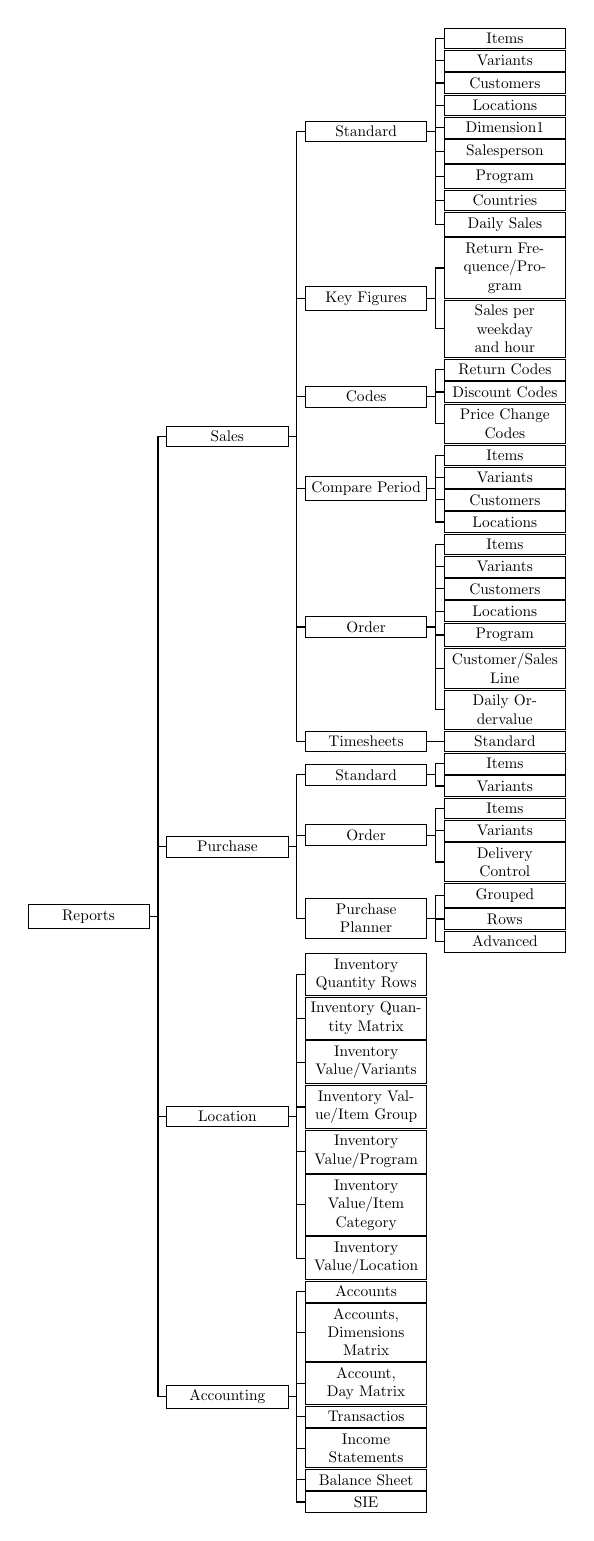
\begin{tikzpicture}[level distance=1.25in,sibling distance=.6pt,scale=.555]

\tikzset{edge from parent/.style= 
            {thick, draw,
                edge from parent fork right},every tree node/.style={draw,minimum width=1in,text width=1in, align=center},grow'=right}
\Tree 
    [. Reports 
        [.{Sales}
            [.{Standard} 
				[.{Items} ]
            	[.{Variants} ]
            	[.{Customers} ]
            	[.{Locations} ]
            	[.{Dimension1} ]
            	[.{Salesperson} ]
            	[.{Program} ]
            	[.{Countries} ]
            	[.{Daily Sales} ]                        
            ]
            [.{Key Figures} 
				[.{Return Frequence/Program} ]
            	[.{Sales per weekday and hour } ]            
            ]
            [.{Codes} 
            	[.{Return Codes} ]
            	[.{Discount Codes} ]
            	[.{Price Change Codes} ]                   
            ]
            [.{Compare Period} 
				[.{Items} ]
            	[.{Variants} ]
            	[.{Customers} ]
            	[.{Locations} ]             
            ]
            [.{Order} 
				[.{Items} ]
            	[.{Variants} ]
            	[.{Customers} ]
            	[.{Locations} ]  
            	[.{Program} ]
             	[.{Customer/Sales Line} ]
            	[.{Daily Ordervalue} ]          
            ]
            [.{Timesheets}
            	[.{Standard} ]                
            ]
        ]
        [.Purchase
            [.{Standard} 
				[.{Items} ]
            	[.{Variants} ]            
            ]
            [.{Order} 
				[.{Items} ]
            	[.{Variants} ]
	           	[.{Delivery Control} ]            
            ]
            [.{Purchase Planner} 
				[.{Grouped} ]
            	[.{Rows} ]
	           	[.{Advanced} ]              
            ]
        ] 
        [.Location 
        	[.{Inventory Quantity Rows} ]
            [.{Inventory Quantity Matrix} ]
            [.{Inventory Value/Variants} ]
            [.{Inventory Value/Item Group} ]
            [.{Inventory Value/Program} ]
            [.{Inventory Value/Item Category} ]
            [.{Inventory Value/Location} ]
        ]
        [.Accounting 
			[.{Accounts} ]
            [.{Accounts, Dimensions Matrix} ]
            [.{Account, Day Matrix} ]
            [.{Transactios} ]
            [.{Income Statements} ]
            [.{Balance Sheet} ]
            [.{SIE} ]        
        ]
    ]
\end{tikzpicture}
\caption{The different BI-reports available in \bex Online}
\label{fig:BI}
\end{figure}

\begin{figure}
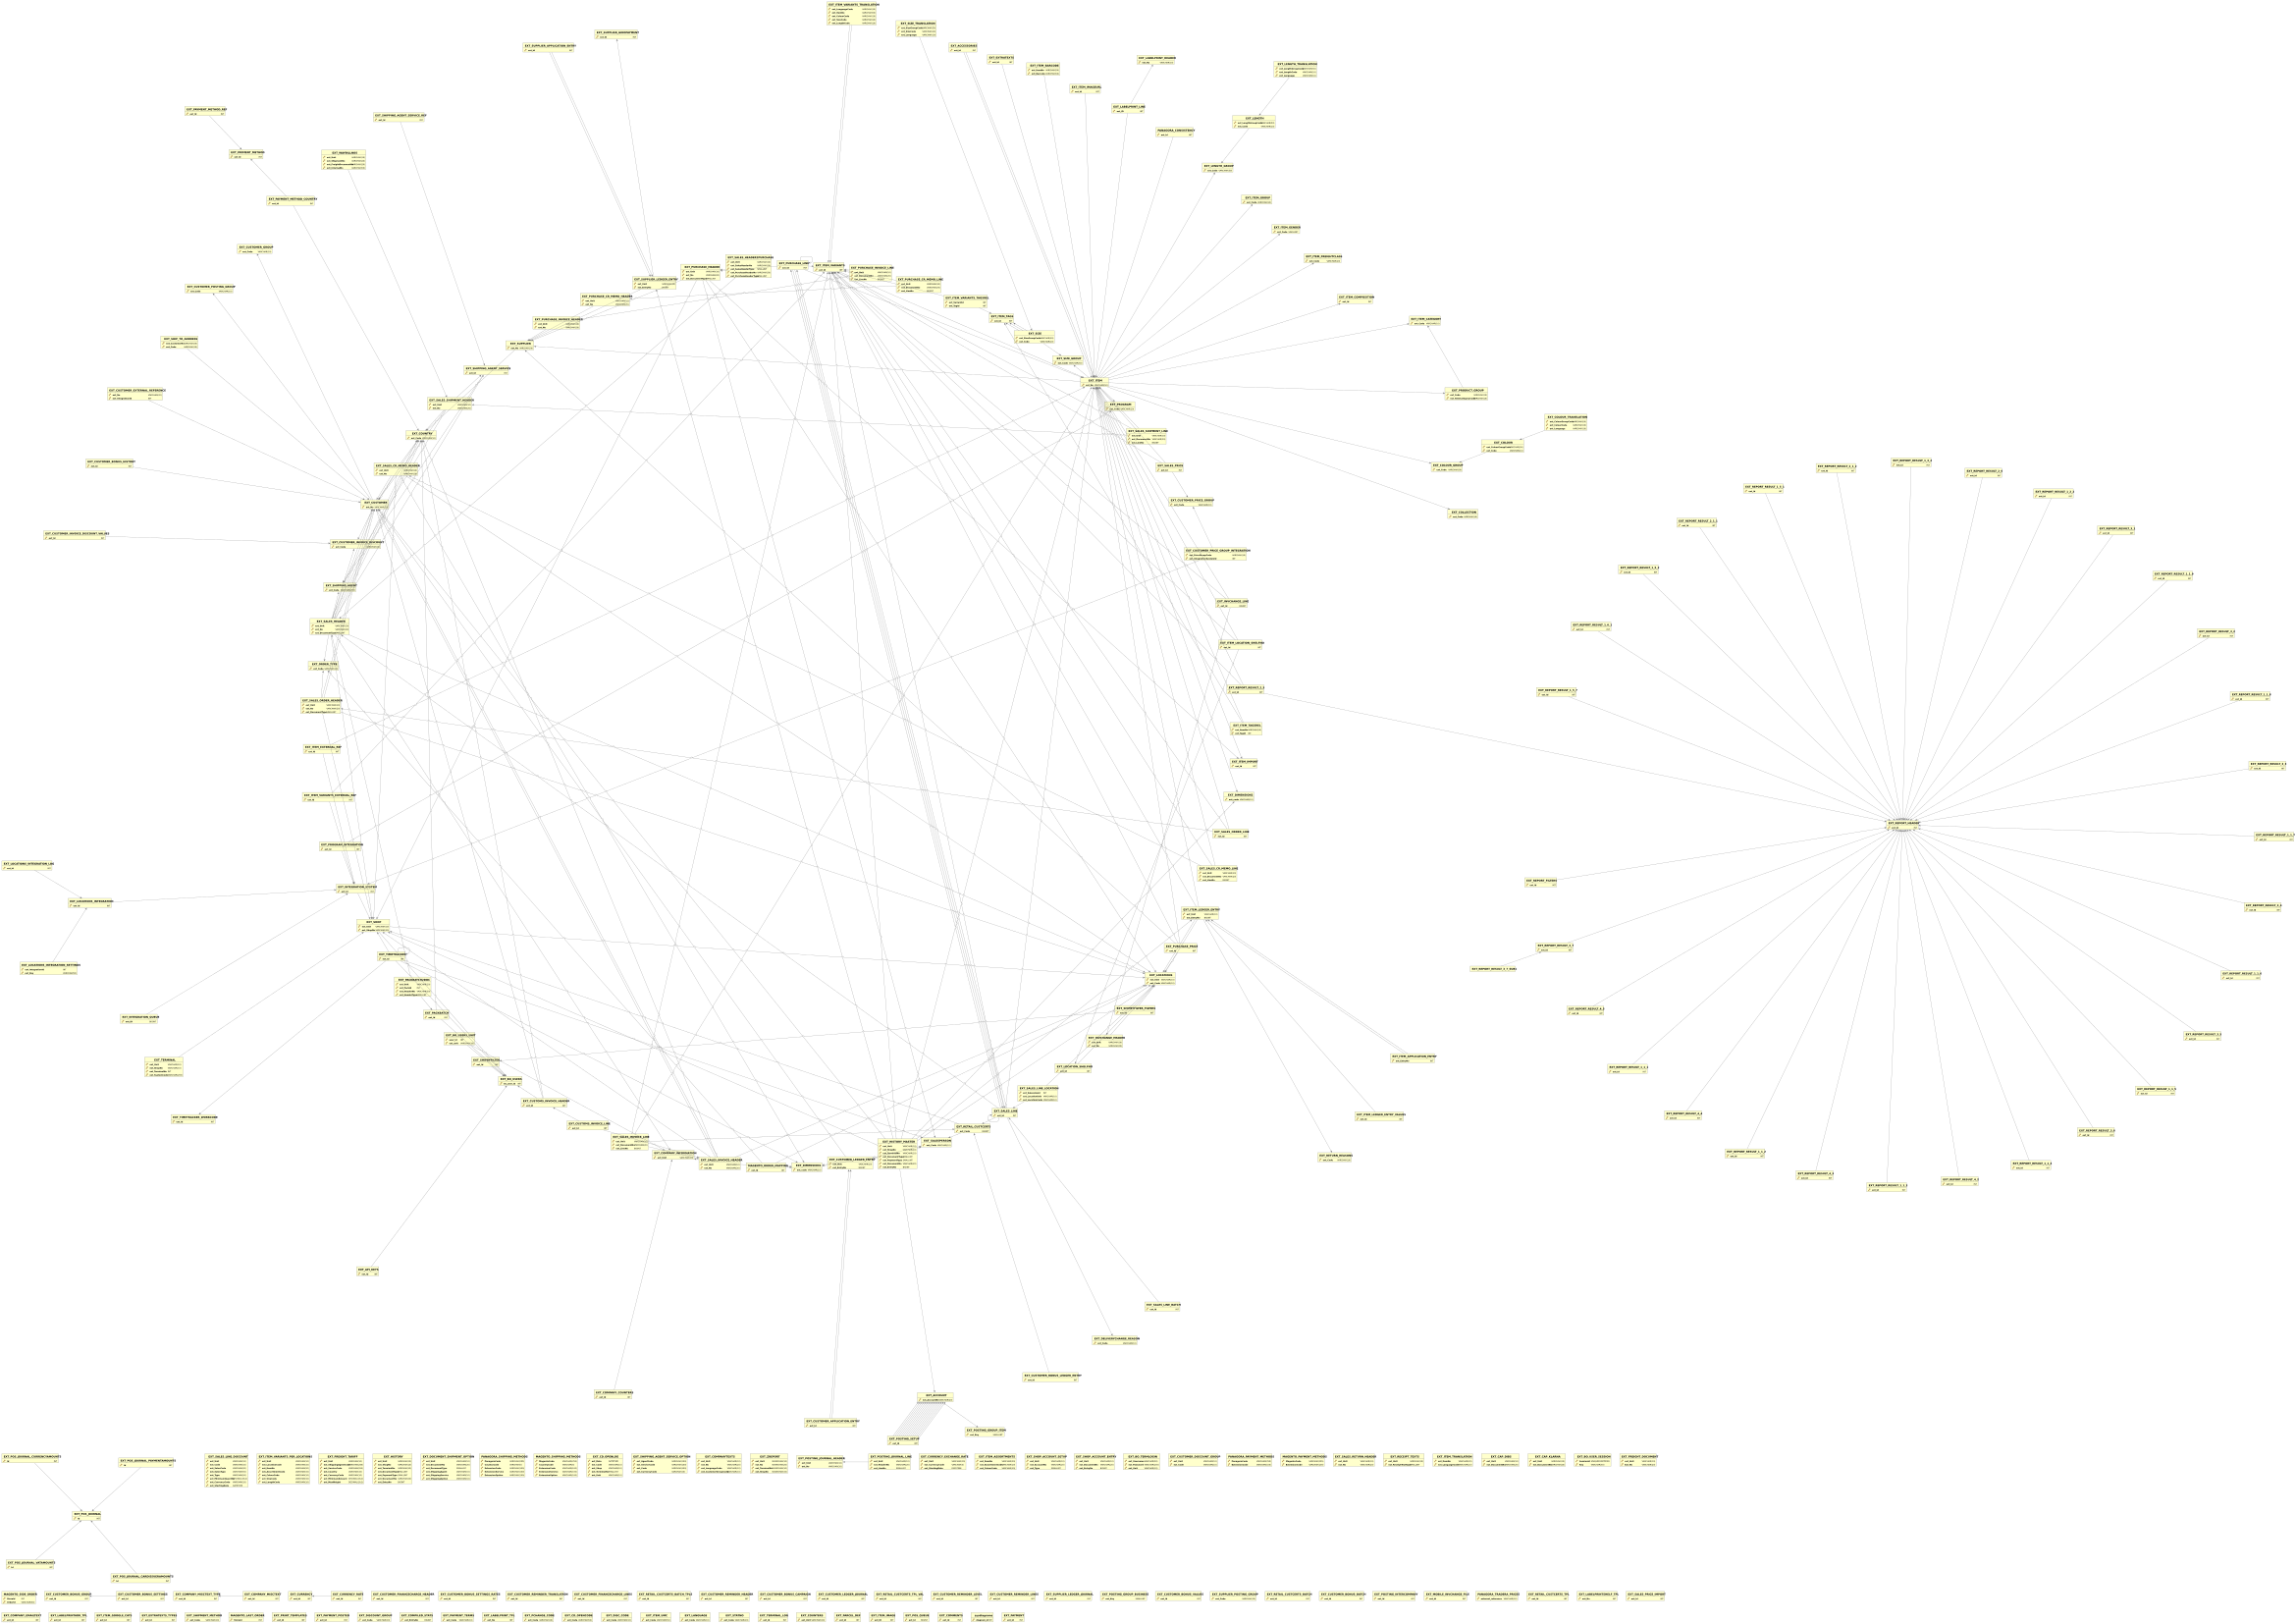
\includegraphics[angle = 270, width = \textwidth]{Pictures/ER.png}
\caption{ER-diagram of all the tables in the database}
\label{fig:ER}
\end{figure}

\end{appendices}
\end{document}